\documentclass[11pt]{article}

% all packages used by any paper must be listed here
\usepackage{newsdebulletin,times,epsfig,subfigure,wrapfig,algorithmic,color,boxedminipage,graphicx,url}

\usepackage{makecell}
\usepackage{multirow}
\usepackage{booktabs}
\usepackage{amsfonts}
\usepackage{amsmath,epsfig}
\usepackage{graphicx}
\usepackage{subfigure}
\usepackage{balance}
\usepackage{xspace,colortbl,subfigure,multirow}
\usepackage{mathrsfs}
\usepackage{amsmath}
\usepackage{cancel}
\usepackage{array}
\usepackage{verbatim}
\usepackage{bbm}
\usepackage{bm}
\usepackage{amsfonts}
\usepackage{color}
\usepackage{eurosym}
\usepackage{setspace,lipsum}
\usepackage{amsmath,amsfonts}
\usepackage{authblk}
%\usepackage{subfig}
\usepackage{url}
\usepackage{multirow}
\usepackage{paralist}
\usepackage{mathtools}
\usepackage{listings}
\usepackage{soul}
\usepackage{enumitem}
\usepackage{fancyvrb}





%\usepackage{algorithm,algorithmicx,algpseudocode} 

%\usepackage[font=small,labelfont=bf]{caption}


\begin{document}

% you may want to put in real date, vol no, issue no- but that is not necessary
\bulletindate{December 2018}
\bulletinvolume{41}
\bulletinnumber{4}
\bulletinyear{2018}

% these are files that I have- but your part of the issue can be done without
% them
\IEEElogo{cs.pdf}
\insidefrontcover{incvA18.pdf}
% \insidebackcover[TCDE Membership Form]{./calls/joinTCDE16.ps}

\begin{bulletin}

%
%  Letters to the editor section.  Use the lettersection environment.
%  Each letter is contained in a letter environment, where the two required
%  options to \begin{letter} are the author and the address of the author.
%

\begin{lettersection}

% there will be other letters- and a blank page will appear in your document
% but the special issue part will be fine

\begin{letter}{Farewell}
{David Lomet}{Microsoft Corporation}
\documentclass[11pt]{article} 

\usepackage{deauthor,times,graphicx}
%\usepackage{url}
\usepackage{hyperref}

\begin{document}


\section*{Farewell}

It was way back in 1992 that Rakesh Agrawal, then the TCDE Chair, appointed me as Editor-in-Chief of the Data Engineering Bulletin. At the time, I saw it as a great opportunity. But it did not occur to me that it would become such an enormous part of my career. Now, 26 years later, it is time, perhaps past time, for me to pass this position on to younger hands, in this case to the capable hands of Haixun Wang. It should not come as a surprise that I am stepping down. Rather, the surprise should be ``why did I stay so long?'' This message is a combination of answer to that question and historical sketch of my time as EIC. These are not unrelated.

When I first became EIC, the Bulletin had already established a reputation as an industry and engineering focused publication, each issue of which was on a special topic.  Won Kim, my predecessor, had very capably established that publication model. Papers are solicited by each issue editor, with the editor selecting which authors to invite. The papers are a mix of work in progress, position statements, surveys, etc. But all focused on the special topic. I was determined not to screw this up. Indeed, I accepted the EIC appointment because I believed that the role that the Bulletin played is unique in our database community.  I stayed so long because I still believe that.  

Over the years, the Bulletin went through several major changes. As early as 1993, the Bulletin could be accessed online as well as via print subscription. This was a major transition. Mark Tuttle, then a colleague of mine in Digital (DEC) Cambridge Research Lab designed the latex style files that enabled this. Shortly thereafter, to economize on costs, the Bulletin became one of the earliest all electronic publications in our field. 

In 1995, hosting the Bulletin web site was provided by Microsoft- continuing until three years ago. Around 2010, the IEEE Computer Society became the primary host for the Bulletin. Around 2000, at the suggestion (prodding) of Toby Lehman,individual articles in addition to complete issues were served from the Bulletin web sites. Over this time, the style files and my procedures for generating the Bulletin evolved as well. Mark Tuttle again, and S. Sudarshan, who had been a Bulletin editor, provided help in evolving procedures used to generate the Bulletin and its individual articles. 

The Computer Society, and specifically staff members John Daniel, Carrie Clark Walsh, and Brookes Little, provided a TCDE email membership list used to distribute issue announcements, as well as helping in myriad other ways. The existence of dbworld (one of Raghu Ramakrishnan enduring contributions) enabled wider announcement distribution to our database community. The cooperation of Michael Ley with the prompt indexing of the Bulletin at dblp both ensured wider readership and provided an incentive for authors to contribute. Over the years, I was given great support by TCDE Chairs, starting with Rakesh Agrawal, then Betty Salzberg, Erich Neuhold, Paul Larson, Kyu-Young Whang, and Xiaofang Zhou. 

The most important part of being Bulletin EIC was the chance to work with truly distinguished members of the database community. It was enormously gratifying to have stars of our field (including eight Codd Award winners- so far) serving as editors. I take pride in appointing several of them as editors prior to their wider recognition.  It is the editors that deserve the credit for producing, over the years, a treasure trove of special issues on technologies that are central to our data engineering field. Superlative editors, and their success in recruiting outstanding authors, is the most important part of the Bulletin's success. Successfully convincing them to serve as editors is my greatest source of pride in the role I played as Bulletin EIC.  

Now I am happy to welcome Haixun to this wonderful opportunity.  Haixun's background includes outstanding successes in both research and industry.  He recently served ably as a Bulletin associate editor for issues on ``Text, Knowledge and Database'' and ``Graph Data Processing''.  His background and prior editorial experience will serve our data engineering community well and ensure the ongoing success of the Bulletin.  I wish him and the Bulletin all the best.

And so ``farewell''.  I will always treasure having served as Bulletin EIC for so many years. It was a rare privilege that few are given. Knowing that we were reaching you with articles that you found valuable is what has made the effort so rewarding to me personally. Thank you all for being loyal readers of the Bulletin. 

\end{document}


\end{letter}
\newpage
\begin{letter}{Letter from the Editor-in-Chief}
{Haixun Wang}{WeWork Corporation}
\documentclass[11pt]{article} 

\usepackage{deauthor,times,graphicx}
%\usepackage{url}
\usepackage{hyperref}

\begin{document}
Around the time we published our last issue in March, the nation went
into a lockdown. Life in the last 3 months has been unprecedented in
many ways. As governments around the world scrambled to fight
coronavirus, people in the scientific community, especially those on
the frontline -- doctors, healthcare professionals, medical staff and
researchers -- made heroic efforts and sacrifices to curb the pandemic
and save lives. The data management and data science communities also
sprang to action immediately. Globally, it is the first time that data
driven approaches are being used at such a large scale toward solving
a common problem. Under this backdrop, in this special issue of the
Data Engineering Bulletin edited by Joseph Gonzalez, we feature 8
papers on the topic of {\it digital contact tracing}, a technique that
may prove crucial in the fight against Covid-19.

This issue also features two opinion pieces. Divyakant Agrawal and Amr
El Abbadi's wake-up call on managing data in an untrusted environment
takes us to the fascinating world of cryptocurrencies and
blockchains. It shows what the database community, which was
responsible for creating and perfecting transaction management and
distributed systems, can learn from the blockchain approach when it
comes to handling untrusted behaviours from the underlying
infrastructure. The second opinion piece, written by Jeffrey
D. Ullman, addresses a question on the mind of every data management
person: What is our role in the machine learning and AI revolution?
Have we missed the boat again and become irrelevant? Ullman's
perspective, illustrated by his remake of the well known Conway Venn
Diagram that illustrates the relationship between computer science,
mathematics \& statistics, and domain knowledge is incisive,
thought-provoking, and entertaining at the same time.
\end{document}


\end{letter}
%
\newpage
%
%% your introductory letter goes here
%

\begin{letter}{Letter from the Special Issue Editor}
{Joseph E. Gonzalez}{University of California at Berkeley\\ Berkeley, CA}
\graphicspath{{letters/}}
\documentclass[11pt]{article} 

\usepackage{deauthor,times,graphicx}
%\usepackage{url}
\usepackage{hyperref}



\begin{document}

Machine learning is rapidly maturing into an engineering discipline at the center of a growing range of applications.
This widespread adoption of machine learning techniques poses a new set challenges around the management of the data, code, models, and their relationship throughout the machine learning life-cycle.
In this issue of the Data Engineering Bulletin we have solicited work from both academic and industrial leaders in the data engineering community that are exploring how data engineering techniques can be used to address the challenges of the machine learning life-cycle.




\begin{figure}[h]
\centering
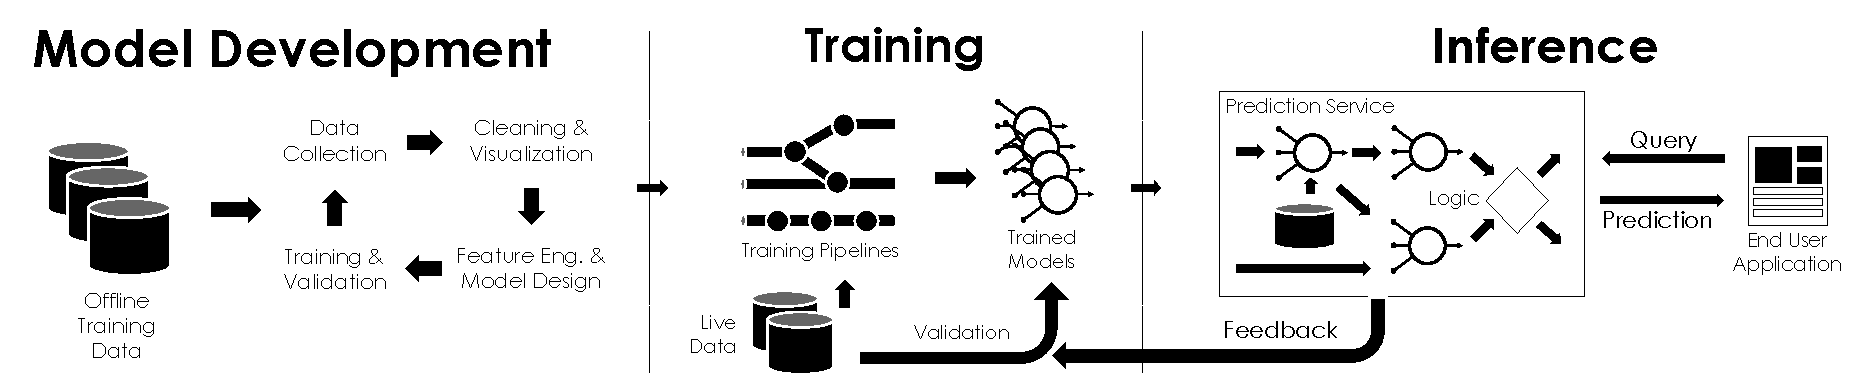
\includegraphics[width=\textwidth]{letters/pipeline.pdf}
\caption{\small \textbf{Machine Learning Life-cycle.} A simplified depiction of the key stages of a machine learning application.}
\label{fig:mllc}
\end{figure}


The machine learning life-cycle (Fig.~\ref{fig:mllc}) spans not only the model development, but also production training and inference.
Each stage demands different skills (e.g., neural network design, data management, and cluster management) and imposes different requirements on the underlying systems.
Yet there is an overwhelming need for unifying design principles and technologies to address pervasive problems including: feature management, data provenance, pipeline reproducibility, low-latency serving, and prediction monitoring just to name a few.


There has been substantial recent progress in systems to aid in managing the machine learning life-cycle.  
Large industrial projects like 
FB Learner Flow 
% \href{https://code.fb.com/core-data/introducing-fblearner-flow-facebook-s-ai-backbone/}{FB Learner Flow}
from Facebook, 
Michelangelo 
% \href{https://eng.uber.com/michelangelo/}{Michelangelo} 
from Uber, and 
TFX 
% \href{https://www.tensorflow.org/tfx/}{TFX} 
from Google have received a considerable of recent attention.  
In this issue we have solicited publications from several more recent industrial and academic projects.

The first paper, by a team at Amazon Research, provides an overview of several real-world use cases and then outlines the key conceptual, data management, and engineering challenges faced in production machine learning systems.
Rather than advocating a single system, this work describes some design principles that can inform potential solutions.


The second and third papers explores the challenges of model management and provenance across the machine learning life-cycle.
They motivate the need for systems to track models and their meta-data to improve reproducibility, collaboration, and governance. 
% expands upon the machine learning life-cycle 
% to include: data preparation, feature engineering, model training, deployment, and maintenance
% and explores the challenges of model 
The second paper introduces, ModelDB, an open-source system for model management and describe some of the functionality and design decisions. 
The third paper describes a related system, ProvDB, that uses a graph data model to capture and query fine-grained versioned lineage of data, scripts, and artifacts throughout the data analysis process.


The fourth paper, by a team at Databricks Inc., describes, MLFlow, a new open-source system to address the challenges of experimentation, reproducibility, and deployment. 
This work leverages containerization to capture the model development environment and a simple tracking API to enable experiment tracking.
The extensible model containerization enables model developers to more easily collaborate around modeling environments and then deploy model containers.


The last paper, by a team at Microsoft, focuses on inference and explores the challenges and opportunities of serving white-box prediction pipelines.  
In contrast to the containerization of pipelines in MLFlow, the Microsoft team leverage knowledge about the internal of the prediction pipeline to more efficient serve predictions. 



\end{document}



\end{letter}

\end{lettersection}



% put the name of your special issue below
\begin{articlesection}{Machine Learning Life-cycle Management}
%
%  Contributed articles section.  Use the articlesection environment.
%  Each article is contained in an article environment, where the two required
%  options to \begin{article} are the title and author of the article
%
%\begin{article}
%{Title of article}
%{list of authors}
%\input{author-name/article.tex}
%\end{article}
\begin{article}
{On Challenges in Machine Learning Model Management}
{Sebastian Schelter, Felix Biessmann, Tim Januschowski, David Salinas, Stephan Seufert, Gyuri Szarvas}
\graphicspath{{submissions/AmazonModelManagement/figs/}}
\documentclass[11pt]{article}
% \usepackage[usenames,dvipsnames,svgnames]{xcolor}

\usepackage{deauthor}
\usepackage{times, enumerate}
\usepackage{graphicx}
\usepackage{authblk}
\usepackage{hyperref,subfigure}
\usepackage{wrapfig}
\usepackage{enumitem}

\graphicspath{{figs/}}



\newcommand{\hdr}[1]{\noindent\textbf{#1.}}

\begin{document}

\title{On Challenges in Machine Learning Model Management}
%
\author{Sebastian Schelter, Felix Biessmann, Tim Januschowski,\\ David Salinas, Stephan Seufert, Gyuri Szarvas \\
{\small \texttt{\{sseb,biessman,tjnsch,dsalina,seufert,szarvasg
\}@amazon.com}}\\
Amazon Research
}

% \affil{{\small \texttt{\{sseb,biessman,tjnsch,dsalina,seufert,szarvasg
% \}@amazon.com}}}
% \affil{Amazon Research}

\maketitle

\begin{abstract}
The training, maintenance, deployment, monitoring, organization and documentation of machine learning (ML) models -- in short model management --
is a critical task in virtually all production ML use cases. Wrong model management decisions can lead to poor performance of a ML system and can result in high maintenance cost. As both research on infrastructure as well as on algorithms is quickly evolving, there is a lack of understanding of challenges and best practices for ML model management. Therefore, this field is receiving increased attention in recent years, both from the data management as well as from the ML community. In this paper, we discuss a selection of ML use cases, develop an overview over conceptual, engineering, and data-processing related challenges arising in the management of the corresponding ML models, and point out future research directions.
\end{abstract}

\section{Introduction}

Software systems that learn from data are being deployed in increasing numbers in industrial application scenarios. Managing these machine learning (ML) systems and the models which they apply imposes additional challenges beyond those of traditional software systems~\cite{Kumar2015,Polyzotis2017,Crankshaw2017}. In contrast to textbook ML scenarios (e.g., building a classifier over a single table input dataset), real-world ML applications are often much more complex, e.g., they require feature generation from multiple input sources, may build ensembles from different models, and frequently target hard-to-optimize business metrics. Many of the resulting challenges caught the interest of the data management research community only recently, e.g., the efficient serving of ML models, the validation of ML models, or machine learning-specific problems in data integration. A major issue is that the behavior of ML systems depends on the data ingested, which can change due to different user behavior, errors in upstream data pipelines, or adversarial attacks to name just some examples~\cite{Baylor2017}. As a consequence, algorithmic and system-specific challenges can often not be disentangled in complex ML applications. Many decisions for designing systems that manage ML models require a deep understanding of ML algorithms and the consequences for the corresponding system. For instance, it can be difficult to appreciate the effort of turning raw data from multiple sources into a numerical format that can be consumed by specific ML models -- yet this is one of the most tedious and time consuming tasks in the context of ML systems~\cite{Stonebraker2018}.

In this paper, we introduce a set of intricate use cases in Section~\ref{sec:usecases}, and elaborate on the corresponding general challenges with respect to model management. We discuss conceptual challenges in Section~\ref{sec:conceptual}, e.g., how to exactly define the model to manage~\cite{Vanschoren2014}, how to validate the predictions of a model both before and after deployment~\cite{Baylor2017}, and how to decide when to retrain a model. Next, we elaborate on data-management related challenges in Section~\ref{sec:datamanagement}. These evolve around the fact that ML models are part of larger ML pipelines, which contain the corresponding feature transformations and related metadata~\cite{Sparks2017,VanDerWeide2017}. Efficient model management requires us to be able to capture and query the semantics, metadata and lineage of such pipelines~\cite{Vartak2016,Schelter2017,Vartak2018}. Unfortunately, this turns out to be a tough problem as there is no declarative abstraction for ML pipelines that applies to all ML scenarios. Finally, we list a set of engineering-related challenges, which originate from a lack of agreed-upon best practices as well as from the difficulties of building complex systems based on components in different programming languages~(Section~\ref{sec:engineering}).

\section{Selected Use Cases}
\label{sec:usecases}

\hdr{Time Series Forecasting} Large-scale time series prediction or \emph{forecasting} problems have received attention from the ML, statistics and econometrics community. The problem of forecasting the future values of a time series arises in numerous scientific fields and commercial applications. In retail, an accurate forecast of product demand can result in significant cost reductions through optimal inventory management and allocation. In modern applications, many time series need to be forecasted for simultaneously. Classical forecasting techniques, such as ARIMA models~\cite{Box2015time}, or exponential smoothing and its state-space formulation~\cite{Hyndman2008forecasting} train a single model per time series.
%
Since these approaches are typically fast to train~\cite{taylor2017forecasting,hyndman2007automatic}, it is possible to retrain the models every time a new forecast needs to be generated. In theory, this would mean that little to no management of the resulting models is required; however, the practice very often differs significantly. While classical forecasting models excel when time series are well-behaved (e.g., when they are regular, have sufficiently long history, are non-sparse), they struggle with many characteristics commonly encountered in real-world use cases such as cold-starts (new products), intermittent time series and short life cycles~\cite{Seeger2016bayesian}. Such complications require models that can transfer information across time series. Even for well-behaved time series, we may often want to be able to learn certain effects (e.g., the promotional uplift in sales) across a number of products. Therefore, forecasting systems in the real-world become quite complex even if the classical models at its core are simple~\cite{Bose2017}. Maintaining, managing, and improving the required ML pipelines in such systems is a non-trivial challenge -- not only in production environments which may require complex ensembles of many simple models, but especially in experimental settings when different individual models are evaluated on different time series. 
%
We found that a natural alternative to such complex ensembles of simple models is end-to-end learning via deep learning models for forecasting~\cite{Faloutsos2018}. Neural forecasting models have the ability to learn complex patterns across time series. They make use of rich metadata without requiring significant manual feature engineering effort~\cite{Flunkert2017}, and therefore generalize well to different forecasting use cases. Modern, general-purpose implementations of neural forecasting mdoels are available in cloud ML services such as \textit{AWS SageMaker}~\cite{janu2018}. However, when such neural forecasting models are deployed in long-running applications, careful management of the resulting models is still a major challenge, e.g., in order to maintain backwards compatibility of the produced models.\\

\hdr{Missing Value Imputation} Very often, ML is leveraged to automatically fix data quality problems. A prominent issue in this context are missing values. A scenario in which missing values are problematic are product catalogs of online retailers. Product data needs to be complete and accurate, otherwise products would not be found by customers. Yet in many cases, product attributes may not be entered by sellers, or they might apply a different schema and semantic, which results in conflicting data that would need to be discarded. Manually curating this data does not scale, hence automatic solutions leveraging ML technology are a promising option for ensuring high data quality standards. While there are many approaches dealing with missing values, most of these methods are designed for matrices only. In many real-world use cases however, data is not available in numeric formats but rather in text form, as categorical or boolean values, or even as images. Hence most datasets must undergo a feature extraction process that renders the data amenable to imputation. Such feature extraction code can be difficult to maintain, and not every data engineer that is facing missing values in a data pipeline will necessarily be able to implement or adapt such code. This is why  implementing the feature extraction steps and the imputation algorithms in one single pipeline (that is learned end-to-end) greatly simplifies model management~\cite{Biessmann2018} for end users. An end-to-end imputation model that uses hyperparameter optimization to automatically perform model selection and parameter tuning can be applied and maintained by data engineers without in depth understanding of all algorithms used for feature extraction and imputation.\\

\hdr{Content Moderation} Another broad set of ML-related tasks can be summarized under the umbrella of content moderation. There is a wide range of such use cases, some simple in their nature (e.\,g., the detection of swear words in content), while others are more complex, e.\,g., the detection of fake news, or the detection of copyright infringement in music or video. As an example, we focus onto user comments in online communities~\cite{contentModeration17}. Before publishing user provided content, moderation might take place, often via a mixture of ML methods and human curators. Common tasks are to mark content which contains inappropriate language or does not adhere to a community standard. Such moderation consists of offline training of models using manually labelled data. However, during the production usage of such models, we need to constantly monitor the model accuracy. A typical approach looks as follows: content that can be classified with high accuracy by automated models does not require a human interaction. However, content for which the model output is inconclusive (for this, probabilistic classifiers are of utmost importance) are directly passed to human annotators. This data can then be used to re-train the model online in an active learning setting. Depending on their overall capacity, we can also randomly select sample content that was classified with high probability. Periodically, we should also select and relabel a completely random subset of the incoming content. In this way, we constantly update the model and improve its performance.\\


\hdr{Automating Model Metadata Tracking} An orthogonal data management use case of great importance in all ML applications is tracking the metadata and lineage of ML models and pipelines. When developing and productionizing ML models, a major proportion of the time is spent on conducting model selection experiments, which consist of training and tuning models and their corresponding features~\cite{Sculley2015,Bose2017,Kumar2015,Polyzotis2017,Zinkevich2017,Baylor2017}. Typically, data scientists conduct this experimentation in their own ad-hoc style without a standardized way of storing and managing the resulting experimentation data and artifacts. As a consequence, the models resulting from these experiments are often not comparable, since there is no standard way to determine whether two models had been trained on the same input data. It is often technically difficult to reproduce successful experiments later in time. To address the aforementioned issues and assist data scientists in their daily tasks, we built a lightweight system for handling the metadata of ML experiments~\cite{Schelter2017}. This system allows for managing the metadata (e.\,g., \textit{Who created the model at what time? Which hyperparameters were used? What feature transformations have been applied?}) and lineage (e.\,g., \textit{Which dataset was the model derived from? Which dataset was used for computing the evaluation data?}) of produced artifacts, and provides an entry point for querying the persisted metadata. Such a system enables regular automated comparisons of models in development to older models, and thereby provides a starting point for quantifying the accuracy improvements that teams achieve over time towards a specific ML goal. The resulting database of experiments and outcomes can furthermore be leveraged later for accelerating meta learning tasks~\cite{Feurer2015}.\\

\section{Model Management Challenges}
\label{sec:challenges}

The aforementioned use cases lead to a number of challenges that we discuss in the following subsections. We categorize the challenges broadly into three categories: (i)~\textit{conceptual challenges}, involving questions such as what is part of a model, (ii)~\textit{data management challenges}, which relate to questions about the abstractions used in ML pipelines and (iii)~\textit{engineering challenges}, such as building systems using different languages and specialized hardware.

\subsection{Conceptual Challenges}
\label{sec:conceptual}

\hdr{Machine Learning Model Definition} It is surprisingly difficult to define the actual model to manage. In the most narrow sense, we could consider the model parameters obtained after training (e.g., the weights of a logistic regression model) to be the model to manage. However, input data needs to be transformed into the features expected by the model. These corresponding feature transformations are an important part of the model that needs to be managed as well. Therefore, many libraries manage ML \textit{pipelines}~\cite{Pedregosa2011,Meng2015} which combine feature transformations and the actual ML model in a single abstraction. There are already established systems for tracking and storing models which allow to associate feature transformations with model parameters~\cite{Vanschoren2014,Vartak2016,Schelter2017}. Due to the i.i.d.-assumption inherent in many ML algorithms, models additionally contain implicit assumptions on the distribution of the data on which they are applied later. Violations of these assumptions (e.g., covariate shift in the data) can lead to decreases in prediction quality. Capturing and managing these implicit assumptions is tricky however, and systematic approaches are in the focus of recent research~\cite{Baylor2017,Hynes2017,Schelter2018}. A further distinction from a systems perspective is whether the model is considered to be a `black-box' with defined inputs and outputs (e.g., a docker image with a REST-API or a scikit-learn pipeline with transformers and estimators) or whether the model is presented in declarative form comprised of operations with known semantics (e.g., the computational graph of a neural network). Even along these outlined dimensions, the heterogeneity of ML models and the complexity of many real-world ML applications render the definition of ML models difficult. For example: How should one handle combinations of models (e.g., in ensembles when models from different languages or libraries are combined, or when an imputation model is part of the preprocessing logic of another model) or meta-models, e.g., meta-learning algorithms or neural architecture searches.\\

\hdr{Model Validation} The ability to back-test the accuracy of models over time is crucial in many real-world usages of ML. Models evolve continuously as data changes, methods improve or software dependencies change. Every time such a change occurs, model performance must be re-validated. These validations introduce a number of challenges and pitfalls: When we compare the performance of ML models, we must ensure that the models have been trained and evaluated using the same training, test and validation set. Additionally, it is crucial that the same code for evaluating metrics is used throughout time and across different models to be able to guarantee comparability. The more experiments we conduct however, the more we risk to overfit on the test or validation data.
%
A further practical problem in backtesting comes from long-running experiments and complex interactions between pipelines of models. A change in backtesting results is often hard to attribute to specific code and configuration changes. Furthermore, in long-existing, highly-tuned ML systems, it is unlikely that the overall accuracy improves significantly. Usually, a new model introduces an improvement but this improvement comes at some cost (such as longer prediction times), which makes wrapping-up release candidates challenging.
%
Specific domains introduce additional challenges. For instance, the train/validation/test split that is required in virtually all ML evaluations is often conducted by randomly partitioning an initial dataset into given proportions, such as 80\%, 10\% and 10\% of the data. In real-world scenarios, in particular in those where the i.i.d.-assumption often made in ML does not hold, we must partition the data more carefully to avoid leakage. For instance in the case of forecasting, it would not be appropriate to split the data per time-series. We need to make sure that no future information such as seasonality is revealed on a training set. Further practical considerations are to consider dynamic backtesting scenarios where we conduct rolling evaluations over time to ensure that our backtest results do not depend on a specific point in time where we performed the split. Each evaluation should track such information in order to always be able to assert that no data leakage happened in a previous evaluation.

In other use cases that involve classification models, such as the imputation of missing values, naive train/test splits can lead to problems as well. Real world datasets often have very skewed distributions of categories. Few categories are observed very often, but many categories are observed only very rarely. Conducting a naive cross-validation split often results in training sets or test sets that contain not enough data for single categories to either train a sensible model or to get a reasonable estimate of the generalization error. 

Apart from validation of models in offline backtests, assessing the performance of models in production is crucial. Making implicit assumptions about data explicit and enabling automatic data validation~\cite{Schelter2018} is even more important in online scoring scenarios. When launching a new model, we can validate its effectiveness in various degrees. Launching the model in ``shadow mode'' (i.e., routing part of the data to the model, but not consuming its output) often helps to catch operational problems. Whenever possible, one should conduct rolling comparisons between ground truth and predictions. A/B or bandit tests are often employed to explose a model in an end-user experience. Note that for forecasting, A/B tests can be quite challenging due to the long and indirect feedback cycles.  Independent of the model launch mechanism, sanity-checking the model output is best practice. Since having high-quality sanity checks in place is as difficult as solving the original ML problem typically, we can employ simple, cheap-to-run or robust prediction models for comparisons, work with thresholding or randomized human inspection. If the core models allows to quantify its reliability via probabilities, this helps in making  more informed choices on the model validity.\\

\hdr{Decisions on Model Retraining} Deciding when to retrain a model is challenging. Training usually is done offline and models are loaded at prediction/inference time in a serving system. If new events occur that our models have not been trained on, we need to trigger retraining or even re-modelling. In the retail demand forecasting domain, examples of such events are the introduction of a new public holiday, a new promotional activity or a weather irregularity. Detecting change in the data is critical, as issues and changes in datasets drastically affect the quality of the model and can invalidate evaluations. When such data changes impact the final metrics (as noticed through backtests), backtracking the root-cause to the dataset is only possible when dataset metadata and lineage have been recorded beforehand.
Similar challenges occur in the imputation use case. Standard cross-validation techniques help to estimate the generalization error and tune precision thresholds for missing value imputation models. But in the presence of noisy training data, it is important to always have some fraction of the predictions audited by human experts and mark imputations as such. When humans are in the loop of such a system, interesting model management challenges can emerge. If auditors are able to update the training data with their audited data, they may often tend to solidarize with the ML pipeline in that they try to increase the model performance as much as they can, which can lead to severe overfitting. As a consequence, everyone involved in the model lifecycle should have a minimal understanding of the caveats of ML systems, such as overfitting. Furthermore, such cases show that it is important to carefully control evaluation and training samples, and guaranteeing this in continuously changing data pipelines can be quite challenging.\\

\hdr{Adversarial Settings} In our exemplary scenario for content moderation in communities, an adversarial setting can occur where malicious users try to understand the boundary conditions of the classifier. For example, users could try to reverse engineer the thresholds under which content is automatically classified and then try to exploit weaknesses of the classifier. In such settings, incoming data will shift over time, which requires careful monitoring of the input and the distribution of the output probabilities. We would assume that more and more content contributions are close to the prediction threshold so that the distribution shifts over time. Once such a distribution shift is deemed to be severe enough, one needs to retrain the model and for this, must obtain new labeled data. Another approach is to rely on active learning. Given a model that outputs a probabilistic classification, it can be constantly updated by acquiring (manually labeled) data from both the decision boundary as well as randomly picked instances. Modeling the adversarial actions themselves by another model is possible in theory and certainly desirable as it eliminates the need to keep labelling data, but in practice, this is often extremely difficult, therefore careful monitoring of the deployed models is crucial.\\


\subsection{Data Management Challenges}
\label{sec:datamanagement}

\hdr{Lack of a Declarative Abstraction for the whole ML Pipeline} A major success factor of relational databases is that that their data processing operations are expressed in a declarative language (SQL) with algebraic properties (relational algebra). This allows the system to inspect computations (e.g., for recording data provenance) and to rewrite them (e.g., for query optimization). Unfortunately, there is a lack of a declarative abstraction for end-to-end ML pipelines. These comprise of heterogenous parts (e.g., data integration, feature transformation, model training) which typically apply different operations based on different abstractions. Loading and joining the initial data applies operations from relational algebra. Feature transformations such as one-hot-encoding categorial variables, feature hashing, and normalization often apply map-reduce like transformations, composed in a `pipeline'-like abstraction popularized by scikit-learn~\cite{Pedregosa2011,Meng2015,Sparks2017}. The actual model training phase uses mostly operations from linear algebra which in many cases require specialized systems and/or hardware to be run efficiently~\cite{Abadi2016,Chen2015}. While general dataflow systems such as Apache Spark support all of the listed phases, it turns out that the dataflow abstraction is very inefficient for many advanced analytics problems~\cite{Mcsherry2015,Boden2017} and most models are implemented as black-boxes in such systems. This led to the development of specialized systems, such as engines for training deep neural networks, that are tailored towards certain learning algorithms (mini-batch stochastic gradient descent) and very efficiently leverage specialized hardware such as GPUs. Unfortunately, these systems do not support general relational operations, e.g., they lack join primitives.  As a consequence, different systems need to be ``glued'' together in many real-world ML deployments, and often require external orchestration frameworks that coordinate the workloads. This situation has tremendous negative effects for model management tasks: It complicates the extraction of metadata corresponding to a particular pipeline (e.g., because the hyperparameters of feature transformations are contained the relational part of pipeline, while hyperparameters for the model training part are found in the computational graph of a neural network), it makes replicability and automation of model selection difficult as many different systems have to be orchestrated, and as a consequence makes it hard to automate model validation.\\

\hdr{Querying Model Metadata} In order to automate and accelerate model lifecycle management, it is of crucial importance to understand metadata and lineage of models (e.g., their hyperparameters, evaluation scores as well as the datasets on which they were trained and validated). This metadata is required for comparing models in order to decide which one to put into production, for getting an overview of team progress, and for identifying pain points as a basis for deciding where to invest tuning efforts. Additionally, a centralized metadata store forms a basis for accelerating learning processes (e.g., through warm-starting of hyperparameter search~\cite{Feurer2015}) and is also helpful for automating certain simple error checks (e.g., ``did someone accidentally evaluate on their training set?''). Unfortunately, many existing ML frameworks have not been designed to automatically expose their metadata. Therefore, metadata capturing systems~\cite{Vanschoren2014,Vartak2016,Schelter2017} in general require that data scientists instrument their code for capturing model metadata, e.g., to annotate hyperparameters of feature transformations or data access operations.  Unfortunately, we found that data scientists often forget to add these annotations or are reluctant to spend the extra effort this imposes. In order to ease the adoption of metadata tracking systems, we explore techniques to automatically extract model metadata from ML applications. In our experience, this works well, as long as certain common abstractions are used in ML pipelines, e.g., `data frames' in pandas or Spark which hold denormalized relational data, and pipelines (in scikit-learn and SparkML) which comprise a way to declare complex feature transformation chains composed of individual operators. For applications built on top of these abstractions, it is relatively simple to automate metadata tracking via reflection and inspection of these components at runtime~\cite{Schelter2017}. In applications not built from declarative components (e.g., systems that rely on shell-scripts to orchestrate model training) on the other hand, it is very hard to automate the metadata extraction process, and a custom component that exposes the metadata has to be built manually. An extension of this problem is that for debugging purposes, often intermediate model outputs need to be inspected~\cite{Zhang2017,Vartak2018}, in addition to model metadata and lineage.

\subsection{Engineering Challenges}
\label{sec:engineering}

\hdr{Multi-Language Code Bases} A hard-to-overcome practical problem in model management originates from the fact that end-to-end ML applications often comprise of components written in different programming languages. Many popular libraries for ML and scientific computations are written in python, often with native extensions. Examples include scikit-learn~\cite{Pedregosa2011}, numpy and scipy as well as the language frontends of major deep learning systems such as MXNet~\cite{Chen2015}, Tensorflow~\cite{Abadi2016} or PyTorch~\cite{Paszke2017}. For data pre-processing, JVM-based systems such as Apache Spark~\cite{Zaharia2012} are often preferred, due to static typing in the language and better support for parallel execution. Such heterogeneous code bases are often hard to keep consistent as automatic refactoring and error checking tools can only inspect either the python or the JVM part of the code, but will not be able to tackle problems across the language barrier. This problem has been identified as ``Multiple-Language Smell''~\cite{Sculley2015} in the past already. Furthermore, such code bases are hard to deploy later on, as they require setups with many different components that need to be orchestrated. E.g., a Spark cluster must be spun up for pre-processing, afterwards the data must be moved to a single machine for model training, and the cluster must be torn down afterwards. An orthogonal problem is the efficient and reliable exchange of data between the components of the system written in different languages. Often, this happens via serialization to a common format on disk, which must be kept in sync. In the future, language-independent columnar memory formats such as Apache Arrow for data or ONNX for neural networks~\cite{ONNX} are promising developments to address this issue.\\

\hdr{Heterogeneous Skill Level of Users} Teams that provide ML technology often have to support users that come from heterogeneous backgrounds. Some user teams have a strong engineering culture, are maintaining large-scale data pipelines and have many job roles dedicated to highly specific tasks. On the other hand, there are product teams with fewer or no members in technical roles. And there are researchers with little experience in handling production systems. ML products should be usable for all customers along this spectrum of technical skills and ensure a smooth transition from one use case to another. The broad range of use cases also requires one to build ML models that work well for large and small datasets at the same time - although these often require different approaches. Some larger datasets can only be tackled with specialized hardware, such as GPUs. But the methods that excel at these tasks with large datasets are often suboptimal when dealing with small data. E.g, if initial training datasets are manually curated by human experts, there is no point in using complex neural network models. In our experience, robust but simple linear models with carefully designed features often work better in these cases. Another dimension that distinguishes the various use cases is how the ML models are deployed afterwards. Some teams might run training and serving using scheduled jobs, but smaller teams often do not want to maintain this type of infrastructure. As a consequence, models have to be designed such that they can be deployed in large-scale scheduled workflows but also quickly tested in experimental prototypes.\\ 

\hdr{Backwards Compatibility of Trained Models} Systems such as Sagemaker~\cite{janu2018} or OpenML~\cite{Vanschoren2014} require backwards compatibility of ML models. A model that was trained last month or last year should still be working today, in particular when trained models might be used in production deployments. Various degrees of backwards compatibility can be satisfied. We may want to impose that the \emph{exact} same result can be obtained, that a \emph{similar} result can be achieved, or in the weakest case that the model can still run. Ensuring those conditions reveals several challenges on model management. Clearly, when a model is deployed and serves predictions, making sure that the exact same result can be retrieved is a strict requirement. To this end, storing all the components defining a model is fundamental in being able to guarantee backwards compatibility and thereby long-term usage. One needs to store at least the data transformations that were required, the implementation of the algorithm, its configuration and finally all its dependencies which can be done by storing model container versions. In the case of training, ensuring that the exact result can be obtained over time may be too strict. This would prevent opportunities to improve models and may be hard to achieve in systems where execution is not fully deterministic (e.g., distributed systems or neural network models when they rely on GPU computation). In such cases, one may prefer to ensure that training results are similar (or better) over time. 

\section{Conclusion}

We introduced a set of ML use cases and discussed the resulting general challenges with respect to model management. Our focus was on conceptual challenges, challenges related to data-management and engineering. Our experience confirms the need for research on data management challenges for model management and ML systems in general~\cite{Sculley2015,Kumar2015}. The problems in this space have their roots in the inherent complexity of ML applications, the lack of a declarative abstraction for end-to-end ML, and the heterogeneity of the resulting code bases. The recent success of deep neural networks in the ML space is often attributed to the gains in prediction accuracy provided by this class of models. We think however that another success factor of neural networks is often overlooked. Neural networks provide an algebraic, declarative abstraction for ML: they are built from computational graphs comprised of tensor operators with clearly defined semantics. Similar to query plans built from relational operators in SQL, this allows for easy combination of complex models and for automatic optimization of the execution on different hardware. With the rise of symbolic neural network APIs it became much simpler for practitioners to experiment with new models, which was one of the main factors contributing to the recent advances we have seen in this field. We strongly feel that the ML space can greatly benefit from adopting proven principles from the data management community such as declarativity and data independence.

Additionally, we observe the rediscovery of many best practices from software engineering and their adaption to managing ML models~\cite{Zinkevich2017}. Examples are scores for quantifying the production-readiness of an ML system~\cite{Breck2016} or unit-tests for the implicit data assumptions inherent in ML models~\cite{Schelter2018}. A promising research direction here is to tackle the challenges stemming from the lack of a common declarative abstraction for end-to-end ML, and to design new languages that support relational algebraic and linear primitives at the same time (and can reason about them them holistically~\cite{Kunft2016,Kunft2017}). Finally, we would like to point out that questions of model management encounter a growing interest in the academic community. Examples of venues for related research are the `Systems for Machine Learning' workshop\footnote{\url{http://learningsys.org}} at the NIPS, ICML and SOSP conferences, the `Data Management for End-to-End Machine Learning' workshop\footnote{\url{http://deem-workshop.org}} at ACM SIGMOD, and the newly formed SysML conference\footnote{\url{http://sysml.cc}}.

% \begin{small}
% 	\bibliographystyle{plain}
% 	\bibliography{on-challenges-in-ml-model-management}
% \end{small}


\begin{thebibliography}{10}

\bibitem{ONNX}
{ONNX} open neural network exchange format, 2017.

\bibitem{Abadi2016}
Mart{\'\i}n Abadi, Paul Barham, Jianmin Chen, Zhifeng Chen, Andy Davis, Jeffrey
  Dean, Matthieu Devin, Sanjay Ghemawat, Geoffrey Irving, Michael Isard, et~al.
\newblock Tensorflow: a system for large-scale machine learning.
\newblock {\em OSDI}, 16:265--283, 2016.

\bibitem{Baylor2017}
Denis Baylor, Eric Breck, Heng-Tze Cheng, Noah Fiedel, Chuan~Yu Foo, Zakaria
  Haque, Salem Haykal, Mustafa Ispir, Vihan Jain, Levent Koc, et~al.
\newblock {TFX: A TensorFlow-Based Production-Scale Machine Learning Platform}.
\newblock {\em KDD}, pages 1387--1395, 2017.

\bibitem{Biessmann2018}
Felix Biessmann, David Salinas, Sebastian Schelter, Philipp Schmidt, and Dustin
  Lange.
\newblock "deep" learning for missing value imputationin tables with
  non-numerical data.
\newblock {\em CIKM}, 2018.

\bibitem{Boden2017}
Christoph Boden, Tilmann Rabl, and Volker Markl.
\newblock Distributed machine learning-but at what cost?
\newblock {\em NIPS Workshop on Machine Learning Systems}, 2017.

\bibitem{Bose2017}
Joos-Hendrik B{\"o}se, Valentin Flunkert, Jan Gasthaus, Tim Januschowski,
  Dustin Lange, David Salinas, Sebastian Schelter, Matthias Seeger, and Yuyang
  Wang.
\newblock {Probabilistic Demand Forecasting at Scale}.
\newblock {\em PVLDB}, 10(12):1694--1705, 2017.

\bibitem{Box2015time}
George E~P Box, Gwilym~M Jenkins, Gregory~C Reinsel, and Greta~M Ljung.
\newblock {\em Time series analysis: forecasting and control}.
\newblock John Wiley \& Sons, 2015.

\bibitem{Breck2016}
Eric Breck, Shanqing Cai, Eric Nielsen, Michael Salib, and D~Sculley.
\newblock What’s your ml test score? a rubric for ml production systems.
\newblock {\em NIPS Workshop on Reliable Machine Learning in the Wild}, 2016.

\bibitem{Chen2015}
Tianqi Chen, Mu~Li, Yutian Li, Min Lin, Naiyan Wang, Minjie Wang, Tianjun Xiao,
  Bing Xu, Chiyuan Zhang, and Zheng Zhang.
\newblock Mxnet: A flexible and efficient machine learning library for
  heterogeneous distributed systems.
\newblock {\em arXiv preprint arXiv:1512.01274}, 2015.

\bibitem{Crankshaw2017}
Daniel Crankshaw, Xin Wang, Guilio Zhou, Michael~J Franklin, Joseph~E Gonzalez,
  and Ion Stoica.
\newblock Clipper: A low-latency online prediction serving system.
\newblock {\em NSDI}, pages 613--627, 2017.

\bibitem{Faloutsos2018}
Christos Faloutsos, Jan Gasthaus, Tim Januschowski, and Yuyang Wang.
\newblock Forecasting big time series: old and new.
\newblock {\em PVLDB}, 11(12):2102--2105, 2018.

\bibitem{Feurer2015}
Matthias Feurer, Jost~Tobias Springenberg, and Frank Hutter.
\newblock Initializing bayesian hyperparameter optimization via meta-learning.
\newblock {\em AAAI}, pages 1128--1135, 2015.

\bibitem{Flunkert2017}
Valentin Flunkert, David Salinas, and Jan Gasthaus.
\newblock Deepar: Probabilistic forecasting with autoregressive recurrent
  networks.
\newblock {\em arXiv preprint arXiv:1704.04110}, 2017.

\bibitem{Hyndman2008forecasting}
Rob Hyndman, Anne~B Koehler, J~Keith Ord, and Ralph~D Snyder.
\newblock {\em Forecasting with exponential smoothing: the state space
  approach}.
\newblock Springer Science \& Business Media, 2008.

\bibitem{hyndman2007automatic}
Rob~J Hyndman, Yeasmin Khandakar, et~al.
\newblock {\em Automatic time series for forecasting: the forecast package for
  R}.
\newblock Number 6/07. Monash University, Department of Econometrics and
  Business Statistics, 2007.

\bibitem{Hynes2017}
Nick Hynes, D~Sculley, and Michael Terry.
\newblock The data linter: Lightweight, automated sanity checking for ml data
  sets.
\newblock {\em NIPS Workshop on Machine Learning Systems}, 2017.

\bibitem{janu2018}
Tim Januschowski, David Arpin, David Salinas, Valentin Flunkert, Jan Gasthaus,
  Lorenzo Stella, and Paul Vazquez.
\newblock Now available in amazon sagemaker: Deepar algorithm for more accurate
  time series forecasting.
\newblock {\em
  https://aws.amazon.com/blogs/machine-learning/now-available-in-amazon-sagemaker-deepar-algorithm-for-more-accurate-time-series-forecasting/},
  2018.

\bibitem{Kumar2015}
Arun Kumar, Robert McCann, Jeffrey Naughton, and Jignesh~M Patel.
\newblock {Model Selection Management Systems: The Next Frontier of Advanced
  Analytics}.
\newblock {\em SIGMOD Record}, 2015.

\bibitem{Kunft2016}
Andreas Kunft, Alexander Alexandrov, Asterios Katsifodimos, and Volker Markl.
\newblock Bridging the gap: towards optimization across linear and relational
  algebra.
\newblock {\em SIGMOD Workshop on Algorithms and Systems for MapReduce and
  Beyond}, 2016.

\bibitem{Kunft2017}
Andreas Kunft, Asterios Katsifodimos, Sebastian Schelter, and Volker Markl.
\newblock Blockjoin: efficient matrix partitioning through joins.
\newblock {\em PVLDB}, 10(13):2061--2072, 2017.

\bibitem{Mcsherry2015}
Frank McSherry, Michael Isard, and Derek~Gordon Murray.
\newblock Scalability! but at what cost?
\newblock {\em HotOS}, 15:14--14, 2015.

\bibitem{Meng2015}
Xiangrui Meng, Joseph Bradley, Burak Yavuz, Evan Sparks, Shivaram Venkataraman,
  Davies Liu, Jeremy Freeman, DB~Tsai, Manish Amde, Sean Owen, et~al.
\newblock {Mllib: Machine learning in apache spark}.
\newblock {\em JMLR}, 17(34):1--7, 2016.

\bibitem{Paszke2017}
Adam Paszke, Sam Gross, Soumith Chintala, Gregory Chanan, Edward Yang, Zachary
  DeVito, Zeming Lin, Alban Desmaison, Luca Antiga, and Adam Lerer.
\newblock Automatic differentiation in pytorch.
\newblock 2017.

\bibitem{contentModeration17}
John Pavlopoulos, Prodromos Malakasiotis, and Ion Androutsopoulos.
\newblock Deeper attention to abusive user content moderation.
\newblock {\em {EMNLP}}, pages 1125--1135, 2017.

\bibitem{Pedregosa2011}
Fabian Pedregosa, Ga{\"e}l Varoquaux, Alexandre Gramfort, Vincent Michel,
  Bertrand Thirion, Olivier Grisel, Mathieu Blondel, Peter Prettenhofer, Ron
  Weiss, Vincent Dubourg, et~al.
\newblock {Scikit-learn: Machine learning in Python}.
\newblock {\em JMLR}, 12:2825--2830, 2011.

\bibitem{Polyzotis2017}
Neoklis Polyzotis, Sudip Roy, Steven~Euijong Whang, and Martin Zinkevich.
\newblock Data management challenges in production machine learning.
\newblock {\em SIGMOD}, pages 1723--1726, 2017.

\bibitem{Schelter2017}
Sebastian Schelter, Joos-Hendrik Boese, Johannes Kirschnick, Thoralf Klein, and
  Stephan Seufert.
\newblock {Automatically Tracking Metadata and Provenance of Machine Learning
  Experiments}.
\newblock {\em NIPS Workshop on Machine Learning Systems}, 2017.

\bibitem{Schelter2018}
Sebastian Schelter, Dustin Lange, Philipp Schmidt, Meltem Celikel, Felix
  Biessmann, and Andreas Grafberger.
\newblock Automating large-scale data quality verification.
\newblock {\em PVLDB}, 11(12):1781--1794, 2018.

\bibitem{Sculley2015}
D~Sculley, Gary Holt, Daniel Golovin, Eugene Davydov, Todd Phillips, Dietmar
  Ebner, Vinay Chaudhary, Michael Young, Jean-Fran{\c{c}}ois Crespo, and Dan
  Dennison.
\newblock {Hidden technical debt in machine learning systems}.
\newblock {\em NIPS}, pages 2503--2511, 2015.

\bibitem{Seeger2016bayesian}
Matthias Seeger, David Salinas, and Valentin Flunkert.
\newblock Bayesian intermittent demand forecasting for large inventories.
\newblock {\em NIPS}, pages 4646--4654, 2016.

\bibitem{Sparks2017}
Evan~R Sparks, Shivaram Venkataraman, Tomer Kaftan, Michael~J Franklin, and
  Benjamin Recht.
\newblock Keystoneml: Optimizing pipelines for large-scale advanced analytics.
\newblock {\em ICDE}, pages 535--546, 2017.

\bibitem{Stonebraker2018}
Michael Stonebraker and Ihab~F Ilyas.
\newblock Data integration: The current status and the way forward.
\newblock {\em Data Engineering Bulletin}, 41(2):3--9, 2018.

\bibitem{taylor2017forecasting}
Sean~J Taylor and Benjamin Letham.
\newblock Forecasting at scale.
\newblock {\em The American Statistician}, 2017.

\bibitem{VanDerWeide2017}
Tom van~der Weide, Dimitris Papadopoulos, Oleg Smirnov, Michal Zielinski, and
  Tim van Kasteren.
\newblock Versioning for end-to-end machine learning pipelines.
\newblock {\em SIGMOD Workshop on Data Management for End-to-End Machine
  Learning}, page~2, 2017.

\bibitem{Vanschoren2014}
Joaquin Vanschoren, Jan~N Van~Rijn, Bernd Bischl, and Luis Torgo.
\newblock Openml: networked science in machine learning.
\newblock {\em ACM SIGKDD Explorations Newsletter}, 15(2):49--60, 2014.

\bibitem{Vartak2018}
Manasi Vartak, Joana~M F~da Trindade, Samuel Madden, and Matei Zaharia.
\newblock Mistique: A system to store and query model intermediates for model
  diagnosis.
\newblock {\em SIGMOD}, pages 1285--1300, 2018.

\bibitem{Vartak2016}
Manasi Vartak, Harihar Subramanyam, Wei-En Lee, Srinidhi Viswanathan, Saadiyah
  Husnoo, Samuel Madden, and Matei Zaharia.
\newblock Model db: a system for machine learning model management.
\newblock {\em SIGMOD Workshop on Human-In-the-Loop Data Analytics}, page~14,
  2016.

\bibitem{Zaharia2012}
Matei Zaharia, Mosharaf Chowdhury, Tathagata Das, Ankur Dave, Justin Ma, Murphy
  McCauley, Michael~J Franklin, Scott Shenker, and Ion Stoica.
\newblock Resilient distributed datasets: A fault-tolerant abstraction for
  in-memory cluster computing.
\newblock {\em NSDI}, 2012.

\bibitem{Zhang2017}
Zhao Zhang, Evan~R. Sparks, and Michael~J. Franklin.
\newblock Diagnosing machine learning pipelines with fine-grained lineage.
\newblock {\em HPDC}, pages 143--153, 2017.

\bibitem{Zinkevich2017}
Martin Zinkevich.
\newblock Rules of machine learning: Best practices for ml engineering, 2017.
\end{thebibliography}


\end{document}
\end{article}


\begin{article}
{{\sc ModelDB}: Opportunities and Challenges in Managing Machine Learning Models}
{Manasi Vartak, Samuel Madden}
\graphicspath{{submissions/DEB-ModelDB/figs/}}
\pdfminorversion=5
\documentclass[11pt]{article}
\usepackage{deauthor,times,graphicx,caption,microtype}
\usepackage{hyperref}
\usepackage{listings}
\usepackage{booktabs}

\begin{document}

\title{Optimistic Lock Coupling: A Scalable and Efficient General-Purpose Synchronization Method}

\author{Viktor Leis, Michael Haubenschild\raisebox{0.9ex}{$\ast$}, Thomas Neumann\\ Technische Universit{\"a}t M{\"u}nchen \hspace{0.7cm} Tableau Software\raisebox{0.9ex}{$\ast$} \\ {\{leis,neumann\}{@}in.tum.de} \hspace{0.7cm} {mhaubenschild{@}tableau.com\raisebox{0.9ex}{$\ast$}}}

\maketitle

\begin{abstract}
As the number of cores on commodity processors continues to increase, scalability becomes more and more crucial for overall performance.
Scalable and efficient concurrent data structures are particularly important, as these are often the building blocks of parallel algorithms.
Unfortunately, traditional synchronization techniques based on fine-grained locking have been shown to be unscalable on modern multi-core CPUs.
Lock-free data structures, on the other hand, are extremely difficult to design and often incur significant overhead.

In this work, we make the case for Optimistic Lock Coupling as a practical alternative to both traditional locking and the lock-free approach.
We show that Optimistic Lock Coupling is highly scalable and almost as simple to implement as traditional lock coupling.
Another important advantage is that it is easily applicable to most tree-like data structures.
We therefore argue that Optimistic Lock Coupling, rather than a complex and error-prone custom synchronization protocol, should be the default choice for performance-critical data structures.
\end{abstract}

\section{Introduction}

% more and more cores
Today, Intel's commodity server processors have up to 28 cores and its upcoming microarchitecture will have up to 48 cores per socket~\cite{intel}.
Similarly, AMD currently stands at 32 cores and this number is expected to double in the next generation~\cite{amd}.
Since both platforms support simultaneous multithreading (also known as hyperthreading), affordable commodity servers (with up to two sockets) will soon routinely have between 100 and 200 hardware threads.

% data structure scalability is important
With such a high degree of hardware parallelism, efficient data processing crucially depends on how well concurrent data structures scale.
Internally, database systems use a plethora of data structures like table heaps, internal work queues, and, most importantly, index structures.
Any of these can easily become a scalability (and therefore overall performance) bottleneck on many-core CPUs.

% traditional synchronization: fine-grained locks, slow, cache invalidation
Traditionally, database systems synchronize internal data structures using fine-grained reader/writer locks\footnote{In this work, we focus on data structure synchronization rather than high-level transaction semantics and therefore use the term {\em lock} for what would typically be called {\em latch} in the database literature. We thus follow common computer science (rather than database) terminology.}.
Unfortunately, while fine-grained locking makes lock contention unlikely, it still results in bad scalability because lock acquisition and release require writing to shared memory.
Due to the way cache coherency is implemented on modern multi-core CPUs, these writes cause additional cache misses\footnote{The cache coherency protocol ensures that all copies of a cache line on other cores are invalidated before the write can proceed.} and the cache line containing the lock's internal data becomes a point of physical contention.
As a result, any frequently-accessed lock (e.g., the lock of the root node of a B-tree) severely limits scalability.

% lock-free bw-tree: no more latches, but indirections, extremely complex
Lock-free data structures like the Bw-tree~\cite{DBLP:conf/icde/LevandoskiLS13a} (a lock-free B-tree variant) or the Split-Ordered List~\cite{DBLP:journals/jacm/ShalevS06} (a lock-free hash table) do not acquire any locks and therefore generally scale much better than locking-based approaches (in particular for read-mostly workloads).
However, lock-free synchronization has other downsides:
First, it is very difficult and results in extremely complex and error-prone code (when compared to locking).
Second, because the functionality of atomic primitives provided by the hardware (e.g., atomically compare-and-swap 8 bytes) is limited, complex operations require additional indirections within the data structure.
For example, the Bw-tree requires an indirection table and the Split-Ordered List requires ``dummy nodes'', resulting in overhead due to additional cache misses.

% OLC for the win
In this paper we make the case for {\em Optimistic Lock Coupling (OLC)}, a synchronization method that combines some of the best properties of lock-based and lock-free synchronization.
OLC utilizes a special lock type that can be used in two modes:
The first mode is similar to a traditional mutex and excludes other threads by physically acquiring the underlying lock.
In the second mode, reads can proceed optimistically by validating a version counter that is embedded in the lock (similar to optimistic concurrency control).
The first mode is typically used by writers and the second mode by readers.
Besides this special lock type, OLC is based on the observation that optimistic lock validations can be interleaved/coupled---similar to the pair-wise interleaved lock acquisition of traditional lock coupling.
Hence, the name Optimistic Lock Coupling.

OLC has a number of desirable features:
\begin{itemize}
\item By reducing the number of writes to shared memory locations and thereby avoiding cache invalidations, it {\bf scales well} for most workloads.
\item In comparison to unsynchronized code, it requires few additional CPU instructions making it {\bf efficient}.
\item OLC is {\bf widely applicable} to different data structures. It has already been successfully used for synchronizing binary search trees~\cite{DBLP:conf/ppopp/BronsonCCO10}, tries~\cite{artsync}, trie/B-tree hybrids~\cite{DBLP:dblp_conf/eurosys/MaoKM12}, and B-trees~\cite{buzzword}.
\item In comparison to the lock-free paradigm, it is also {\bf easy to use} and requires few modifications to existing, single-threaded data structures.
\end{itemize}
Despite these positive features and its simplicity, OLC is not yet widely known.
The goal of this paper is therefore to popularize this simple idea and to make a case for it.
We argue that OLC deserves to be widely known.
It is a good default synchronization paradigm---more complex, data structure-specific protocols are seldom beneficial.

The rest of the paper is organized as follows.
Section~\ref{sec:related} discusses related work, tracing the history of OLC and its underlying ideas in the literature.
The core of the paper is Section~\ref{sec:olc}, which describes the ideas behind OLC and how it can be used to synchronize complex data structures.
In Section~\ref{sec:evaluation} we experimentally show that OLC has low overhead and scales well when used to synchronize an in-memory B-tree.
We summarize the paper in Section~\ref{sec:conc}.

\newpage
\section{Related Work}\label{sec:related}

Lock coupling has been proposed as a method for allowing concurrent operations on B-trees in 1977~\cite{DBLP:journals/acta/BayerS77}.
This traditional and still widely-used method, described in detail in Graefe's B-tree survey~\cite{DBLP:journals/ftdb/Graefe11}, is also called ``latch coupling'', ``hand-over-hand locking'', and ``crabbing''.
Because at most two locks are held at-a-time during tree traversal, this technique seemingly allows for a high degree of parallelism---in particular if read/write locks are used to enable inner nodes to be locked in shared mode.
However, as we show in Section~\ref{sec:evaluation}, on modern hardware lock acquisition (even in shared mode) results in suboptimal scalability.

An early alternative from 1981 is a B-tree variant called B-link tree~\cite{DBLP:journals/tods/LehmanY81}, which only holds a single lock at a time.
It is based on the observation that between the release of the parent lock and the acquisition of the child lock, the only ``dangerous'' thing that could have happened is the split of a child node (assuming one does not implement merge operations).
Thus, when a split happens, the key being searched might end up on a neighboring node to the right of the current child node.
A B-link tree traversal therefore detects this condition and, if needed, transparently proceeds to the neighboring node.
Releasing the parent lock early is highly beneficial when the child node needs to be fetched from disk.
For in-memory workloads, however, the B-link tree has the same scalability issues as lock coupling (it acquires just as many locks).

The next major advance, Optimistic Latch-Free Index Traversal (OLFIT)~\cite{DBLP:conf/vldb/ChaHKK01}, was proposed in 2001.
OLFIT introduced the idea of a combined lock/update counter, which we call {\em optimistic lock}. % , for lack of a better name,
Based on these per-node optimistic locks and the synchronization protocol of the B-link tree, OLFIT finally achieves good scalability on parallel processors.
The OLFIT protocol is fairly complex, as it requires both the non-trivial B-link protocol and optimistic locks.
Furthermore, like the B-link tree protocol, it does not support merging nodes, and is specific to B-trees (cannot easily be applied to other data structures).

In the following two decades, the growth of main-memory capacity led to much research into other data structures besides the venerable B-tree.
Particularly relevant for our discussion is Bronson et al.'s~\cite{DBLP:conf/ppopp/BronsonCCO10} concurrent binary search tree, which is based on optimistic version validation and has a sophisticated, data structure-specific synchronization protocol.
To the best of our knowledge, this 2010 paper is the first that, as part of its protocol, interleaves version validation across nodes---rather than validating each node separately like OLFIT.
In that paper, this idea is called ``hand-over-hand, optimistic validation'', while we prefer the term Optimistic Lock Coupling to highlight the close resemblance to traditional lock coupling.
Similarly, Mao et al.'s~\cite{DBLP:dblp_conf/eurosys/MaoKM12} Masstree (a concurrent hybrid trie/B-tree) is also based on the same ideas, but again uses them as part of a more complex protocol.

The Adaptive Radix Tree (ART)~\cite{art} is another recent in-memory data structure, which we proposed in 2013.
In contrast to the two data structures just mentioned, it was originally designed with single-threaded performance in mind without supporting concurrency.
To add support for concurrency, we initially started designing a custom protocol called Read-Optimized Write Exclusion (ROWEX)~\cite{artsync}, which turned out to be non-trivial and requires modifications of the underlying data structure\footnote{Note that ROWEX is already easier to apply to existing data structures than the lock-free approach. The difficulty depends on the data structure. Applying ROWEX is hard for B-trees with sorted keys and fairly easy for copy-on-write data structures like the Height Optimized Trie~\cite{hot}---with ART being somewhere in the middle.}.
However, fairly late in the project, we also realized, that OLC {\em alone} (rather than as part of a more complex protocol) is sufficient to synchronize ART.
No other changes to the data structure were necessary.
Both approaches were published and experimentally evaluated in a followup paper~\cite{artsync}, which shows that, despite its simplicity, OLC is efficient, scalable, and generally outperforms ROWEX.

Similar results were recently published regarding B-trees~\cite{buzzword}.
In this experimental study a simple OLC-based synchronization outperformed the Bw-tree~\cite{DBLP:conf/icde/LevandoskiLS13a}, a complex lock-free synchronization approach.
Another recent paper shows that for write-intensive workloads, locking often performs better than lock-free synchronization~\cite{DBLP:conf/cidr/FaleiroA17}.
These experiences indicate that OLC is a general-purpose synchronization paradigm and motivate the current paper.

%foster b-tree\cite{DBLP:journals/tods/GraefeKK12}
%Shasha theory~\cite{DBLP:journals/tods/ShashaG88}

\section{Optimistic Lock Coupling}\label{sec:olc}

% locks suck
The standard technique for inter-thread synchronization is mutual exclusion using fine-grained locks.
In a B-tree, for example, every node usually has its own associated lock, which is acquired before accessing that node.
The problem of locking on modern multi- and many-core processors is that lock acquisition and release require writing to the shared memory location that implements the lock.
This write causes exclusive ownership of the underlying cache line and invalidates copies of it on all other processor cores.
For hierarchical, tree-like data structures, the lock of the root node becomes a point of physical contention---even in read-only workloads and even when read/write locks are used.
Depending on the specific data structure, number of cores, cache coherency protocol implementation, cache topology, whether Non-Uniform Memory Access (NUMA) is used, locking can even result in multi-threaded performance that is worse than single-threaded execution.

% in b-trees this happens very much
The inherent pessimism of locking is particularly unfortunate for B-trees:
Despite the fact that logical modifications of the root node are very infrequent, every B-tree operation must lock the root node during tree traversal\footnote{To a lesser extent this obviously applies to all inner nodes, not just the root.}.
Even the vast majority of update operations (with the exception of splits and merges), only modify a single leaf node.
These observations indicate that a more optimistic approach, which does not require locking inner nodes, would be very beneficial for B-trees.

\subsection{Optimistic Locks}

% optimism to the rescue
As the name indicates, optimistic locks try to solve the scalability issues of traditional locks using an optimistic approach.
Instead of always physically acquiring locks, even for nodes that are unlikely to be modified simultaneously, after-the-fact validation is used to detect conflicts.
This is done by augmenting each lock with a version/update counter that is incremented on every modification.
Using this version counter, readers can optimistically proceed before validating that the version did not change to ensure that the read was safe.
If validation fails, the operation is restarted.

% details on opt locks
Using optimistic locks, a read-only node access (i.e., the majority of all operations in a B-tree) does not acquire the lock and does not increment the version counter.
Instead, it performs the following steps:
\begin{enumerate}
\item read lock version (restart if lock is not free)
\item access node
\item read the version again and validate that it has not changed in the meantime
\end{enumerate}
If the last step (the validation) fails, the operation has to be restarted.
Write operations, on the other hand, are more similar to traditional locking:
\begin{enumerate}
\item acquire lock (wait if necessary)
\item access/write to node
\item increment version and unlock node
\end{enumerate}
Writes can therefore protect a node from other writes.

% similar to locks
As we observed in an earlier paper~\cite{artsync}, because of similar semantics, optimistic locks can be hidden behind an API very similar to traditional read/write locks.
Both approaches have an exclusive lock mode, and acquiring a traditional lock in shared mode is analogous to optimistic version validation.
Furthermore, like with some implementations of traditional read/write locks, optimistic locks allow upgrading a shared lock to an exclusive lock.
Lock upgrades are, for example, used to avoid most B-tree update operations from having to lock inner nodes.
In our experience, the close resemblance of optimistic and traditional locks simplifies the reasoning about optimistic locks;
one can apply similar thinking as in traditional lock-based protocols.

\subsection{Lock Coupling with Optimistic Locks}

\begin{figure}
  \centering
  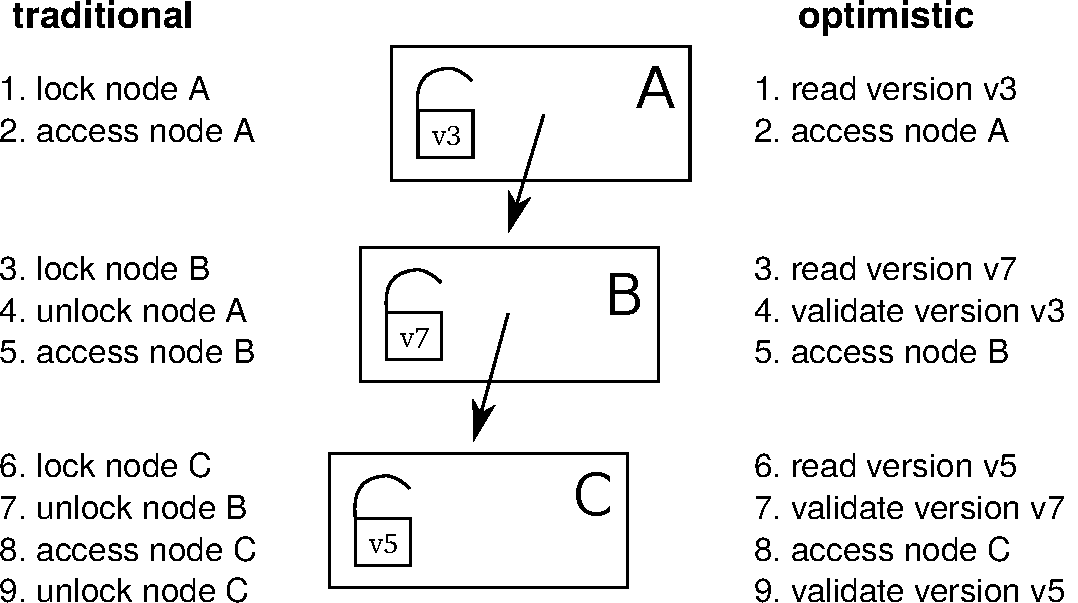
\includegraphics[width=0.65\linewidth]{olcall.pdf}
  \vspace{0.2cm}
  \caption{Comparison of a lookup operation in a 3-level tree using traditional lock coupling (left-hand side) vs.~optimistic lock coupling (right-hand side).}
  \label{fig:olc}
\end{figure}

The traditional and most common lock-based synchronization protocol for B-trees is lock coupling, which interleaves lock acquisitions while holding at most two locks at a time.
If, as we observed earlier, optimistic locks have similar semantics as traditional locks, it is natural to ask whether lock coupling can be combined with optimistic locks.
And indeed the answer is yes: One can almost mechanically translate traditional lock coupling code to optimistic lock coupling code.
This is illustrated in Figure~\ref{fig:olc}, which compares the traversal in a tree of height 3 using traditional and optimistic locks.
As the figure shows, the main difference is that locking is translated to reading the version and that unlocking becomes validation of the previously read version.
This simple change provides efficient lock-free tree traversal without the need to design a complex synchronization protocol.

It is important to emphasize the conceptual simplicity of OLC in comparison to data structures that use custom protocols like the Bw-tree~\cite{DBLP:conf/icde/LevandoskiLS13a}.
To implement lock-free access, the Bw-tree requires an indirection table, delta nodes, complex splitting and merging logic, retry logic, etc.
OLC, on the other hand, can directly be applied to B-trees mostly by adding the appropriate optimistic locking code and without modifying the node layout itself.
Therefore, OpenBw-Tree, an open source implementation of the Bw-tree, requires an order of magnitude more code than a B-tree based on OLC\footnote{Both implementations are available on GitHub: \url{https://github.com/wangziqi2016/index-microbench}}.
Given how difficult it is to develop, validate, and debug lock-free code, simplicity is obviously a major advantage.

\subsection{Correctness Aspects}

\begin{figure}
  % \centering
  %[basicstyle=\normalsize\ttfamily,showstringspaces=false,columns=fullflexible,breaklines=false,breakatwhitespace=true,numbers=none,numberstyle=\small,style=C,keepspaces=true]
\begin{lstlisting}[basicstyle=\ttfamily,language=C++,numbers=left,numberstyle=\small]
std::atomic<BTreeNode*> root;

// search for key in B+tree, returns payload in resultOut
bool lookup(Key key, Value& resultOut) {
   BTreeNode* node = root.load();
   uint64_t nodeVersion = node->readLockOrRestart();
   if (node != root.load()) // make sure the root is still the root
      restart();

   BTreeInner<Key>* parent = nullptr;
   uint64_t parentVersion = 0;

   while (node->isInner()) {
      auto inner = (BTreeInner*)node;

      // unlock parent and make current node the parent
      if (parent)
         parent->readUnlockOrRestart(parentVersion);
      parent = inner;
      parentVersion = nodeVersion;

      // search for next node
      node = inner->findChild(key);
      // validate 'inner' to ensure that 'node' pointer is valid
      inner->checkOrRestart(nodeVersion);
      // now it safe to dereference 'node' pointer (read its version)
      nodeVersion = node->readLockOrRestart();
   }

   // search in leaf and retrieve payload
   auto leaf = (BTreeLeaf*)node;
   bool success = leaf->findValue(key, resultOut);

   // unlock everything
   if (parent)
      parent->readUnlockOrRestart(parentVersion);
   node->readUnlockOrRestart(nodeVersion);

   return success;
}
\end{lstlisting}
  \vspace{0.2cm}
  \caption{B-tree lookup code using OLC. For simplicity, the restart logic is not shown.}
  \label{fig:lookup}
\end{figure}

So far, we have introduced the high-level ideas behind OLC and have stressed its similarity to traditional lock coupling.
Let us now discuss some cases where the close similarity between lock coupling and OLC breaks down.
To make this more concrete, we show the B-tree lookup code in Figure~\ref{fig:lookup}.
In the code, \texttt{readLockOrRestart} reads the lock version and \texttt{readUnlockOrRestart} validates that the read was correct.

One issue with OLC is that any pointer speculatively read from a node may point to invalid memory (if that node is modified concurrently).
Dereferencing such a pointer (e.g., to read its optimistic lock), may cause a segmentation fault or undefined behavior.
In the code shown in Figure~\ref{fig:lookup}, this problem is prevented by the extra check in line 25, which ensures that the read from the node containing the pointer was correct.
Without this additional validation, the code would in line 27 dereference the pointer speculatively read in line 23.
Note that the implementation of \texttt{checkOrRestart} is actually identical to \texttt{readUnlockOrRestart}.
We chose to give it a different name to highlight the fact that this extra check would not be necessary with read/write locks.

Another potential issue with optimistic locks is code that does not terminate.
Code that speculatively accesses a node, like an intra-node binary search, should be written in a way such that it always terminates---even in the presence of concurrent writes.
Otherwise, the validation code that detects the concurrent write will never run.
The binary search of a B-tree, for example, needs to be written in such a way that each comparison makes progress.
For some data structures that do not require loops in the traversal code (like ART) termination is trivially true.

\subsection{Implementation Details}

% implementation, efficiency
To implement an optimistic lock, one can combine the lock and the version counter into a single 64-bit\footnote{Even after subtracting one bit for the lock status, a back-of-the-envelope calculation can show that 63 bits are large enough to never overflow in practice.} word~\cite{artsync}.
A typical read operation will therefore merely consist of reading this version counter atomically.
In C++11 this can be implemented using the \texttt{std::atomic} type.

On x86, atomic reads are cheap because of x86's strong memory order guarantees.
No memory fences are required for sequentially-consistent loads, which are translated (by both GCC and clang) into standard \texttt{MOV} instructions.
Hence, the only effect of \texttt{std::atomic} for loads is preventing instruction re-ordering.
This makes version access and validation cheap.
Acquiring and releasing an optimistic lock in exclusive mode has comparable cost to a traditional lock:
A fairly expensive sequentially-consistent store is needed for acquiring a lock, while a standard \texttt{MOV} suffices for releasing it.
A simple sinlock-based implementation of optimistic locks can be found in the appendix of an earlier paper~\cite{artsync}.

OLC code must be able to handle restarts since validation or lock upgrade can fail due to concurrent writers.
Restarts can easily be implemented by wrapping the data structure operation in a loop (for simplicity not shown in Figure~\ref{fig:lookup}).
Such a loop also enables limiting the number of optimistic retry operations and falling back to pessimistic locking in cases of very heavy contention.
The ability to fall back to traditional locking is a major advantage of OLC in terms of robustness over lock-free approaches, which do not have this option.

In addition to the optimistic shared mode and the exclusive mode, optimistic locks also support a ``shared pessimistic'' mode, which physically acquires the lock in shared mode (allowing multiple concurrent readers but no writers).
This mode is useful for table (or range) scans that touch many tuples on a leaf page (which would otherwise easily abort).
Finally, let us mention that large range scans and table scans, should be broken up into several per-node traversals as is done in the LeanStore~\cite{leanstore} system.

Like all lock-free data structures, but unlike traditional locking and Hardware Transactional Memory~\cite{DBLP:conf/hpca/KarnagelDRLLSL14,DBLP:journals/pvldb/MakreshanskiLS15,htmtkde}, OLC requires care when deleting (and reusing) nodes.
The reason is that a deleting thread can never be sure that a node can be reclaimed because other threads might still be optimistically reading from that node.
Therefore, standard solutions like epoch-based reclamation~\cite{DBLP:conf/sosp/TuZKLM13}, hazard pointers~\cite{DBLP:journals/tpds/Michael04}, or optimized hazard pointers~\cite{DBLP:conf/spaa/BalmauGHZ16} need to be used.
These memory reclamation techniques are, however, largely orthogonal to the synchronization protocol itself.

%-lock-free is not a strong guarantee

\newpage
\section{Evaluation}\label{sec:evaluation}

Let us now experimentally evaluate the overhead and scalability of OLC.
For the experiments, we use an in-memory B+tree implemented in C++11 using templates, which is configured to use nodes of 4096 bytes, random 8 byte keys, and 8 byte payloads.
Based on this B-tree, we compare the following synchronization approaches:
\begin{itemize}
\item an OLC implementation\footnote{An almost identical OLC implementation is available on github: \url{https://github.com/wangziqi2016/index-microbench/tree/master/BTreeOLC}}
\item a variant based on traditional lock coupling and read/write locks
\item the unsynchronized B-tree, which obviously is only correct for read-only workloads but allows measuring the overhead of synchronization
\end{itemize}
Note that earlier work has compared the OLC implementation with a Bw-tree implementation~\cite{buzzword} and other state-of-the-art in-memory index structures.

We use a Haswell EP system with an Intel Xeon E5-2687W v3 CPU, which has 10 cores (20 ``Hyper-Threads'') and 25~MB of L3 cache.
The system is running Ubuntu 18.10 and we use GCC 8.2.0 to compile our code.
The CPU counters are obtained using the Linux perf API\footnote{We use the following convenience wrapper: \url{https://github.com/viktorleis/perfevent}}.

\begin{table}
  \caption{Performance and CPU counters for lookup and insert operations in a B-tree with 100M keys. We perform 100M operations and normalize the CPU counters by that number.}
  \label{tab:overhead}
  \centering
  \begin{tabular}{lrrrrrrr}\toprule
                    &         &        &        & instruc-  & L1     & L3     & branch \\
                    & threads & M op/s & cycles & tions & misses & misses & misses \\\midrule
lookup (no sync.)   & 1       & 1.72   & 2028   & 283     & 39.1   & 14.9   & 16.1   \\
lookup (OLC)        & 1       & 1.65   & 2107   & 370     & 43.9   & 15.1   & 16.7   \\
lookup (lock coup.) & 1       & 1.72   & 2078   & 365     & 42.3   & 16.9   & 15.7   \\\midrule
insert (no sync.)   & 1       & 1.51   & 2286   & 530     & 59.8   & 31.1   & 17.3   \\
insert (OLC)        & 1       & 1.50   & 2303   & 629     & 61.2   & 31.1   & 16.5   \\
insert (lock coup.) & 1       & 1.41   & 2473   & 644     & 61.0   & 31.0   & 17.2   \\\midrule
lookup (no sync.)   & 10      & 15.48  & 2058   & 283     & 38.6   & 15.5   & 16.0   \\
lookup (OLC)        & 10      & 14.60  & 2187   & 370     & 43.8   & 15.8   & 16.8   \\
lookup (lock coup.) & 10      & 5.71   & 5591   & 379     & 54.2   & 17.0   & 14.8   \\\midrule
insert (no sync.)   & 10      & -      & -      & -       & -      & -      & -      \\
insert (OLC)        & 10      & 10.46  & 2940   & 656     & 62.0   & 32.5   & 16.8   \\
insert (lock coup.) & 10      & 7.55   & 4161   & 667     & 75.0   & 28.6   & 16.2   \\
    \bottomrule
\end{tabular}
\end{table}

Table~\ref{tab:overhead} compares the performance and CPU counters for lookup and insert operations in a B-tree with 100M keys.
With {\em single-threaded} execution, we observe that all three approaches have very similar performance.
Adding traditional or optimistic locks to unsynchronized B-tree code results in up to 30\% of additional instructions without affecting single-threaded performance much.

\begin{figure}
  \centering
  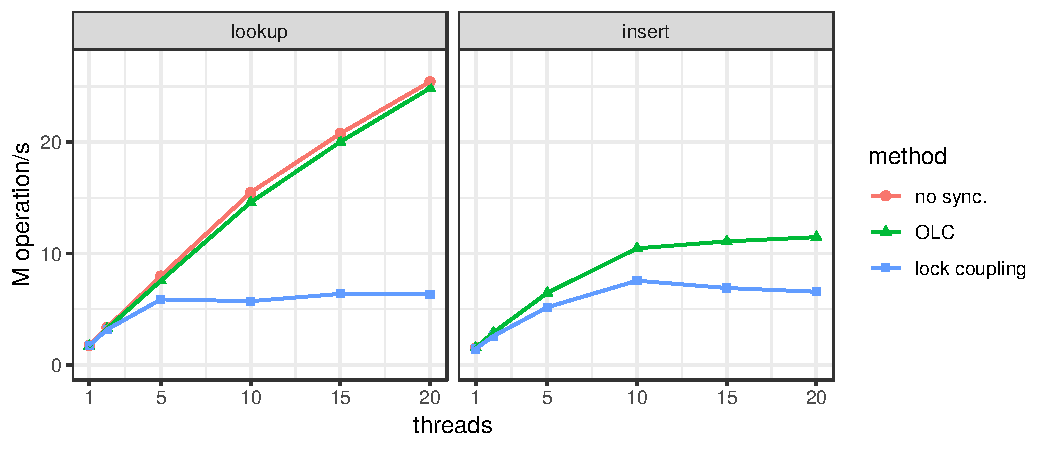
\includegraphics[width=\linewidth]{scale.pdf}
  \vspace{0.2cm}
  \caption{Scalability on 10-core system for B-tree operations (100M values).}
  \label{fig:scale}
\end{figure}

As Figure~\ref{fig:scale} shows, the results change dramatically once we use multiple threads.
For lookup, the scalability of OLC is near-linear up to 20 threads, even though the system has only 10 ``real cores''.
The OLC scalability for insert is also respectable (though not quite as linear because multi-threaded insertion approaches the memory bandwidth of our processor).
The figure also shows that the results of traditional lock coupling with read/write locks are significantly worse than OLC.
With 20 threads, lookup with OLC is 3.9$\times$ faster than traditional lock coupling.

\section{Summary}\label{sec:conc}

Optimistic Lock Coupling (OLC) is an effective synchronization method that combines the simplicity of traditional lock coupling with the superior scalability of lock-free approaches.
OLC is widely applicable and has already been successfully used to synchronize several data structures, including B-trees, binary search trees, and different trie variants.
These features make it highly attractive for modern database systems as well as performance-critical systems software in general.

\begin{thebibliography}{10}

\bibitem{DBLP:conf/spaa/BalmauGHZ16}
O.~Balmau, R.~Guerraoui, M.~Herlihy, and I.~Zablotchi.
\newblock Fast and robust memory reclamation for concurrent data structures.
\newblock In {\em SPAA}, 2016.

\bibitem{DBLP:journals/acta/BayerS77}
R.~Bayer and M.~Schkolnick.
\newblock Concurrency of operations on {B}-trees.
\newblock {\em Acta Informatica}, 9, 1977.

\bibitem{hot}
R.~Binna, E.~Zangerle, M.~Pichl, G.~Specht, and V.~Leis.
\newblock {HOT}: A height optimized trie index for main-memory database
  systems.
\newblock In {\em SIGMOD}, 2018.

\bibitem{DBLP:conf/ppopp/BronsonCCO10}
N.~G. Bronson, J.~Casper, H.~Chafi, and K.~Olukotun.
\newblock A practical concurrent binary search tree.
\newblock In {\em PPOPP}, 2010.

\bibitem{DBLP:conf/vldb/ChaHKK01}
S.~K. Cha, S.~Hwang, K.~Kim, and K.~Kwon.
\newblock Cache-conscious concurrency control of main-memory indexes on
  shared-memory multiprocessor systems.
\newblock In {\em VLDB}, 2001.

\bibitem{intel}
I.~Cutress.
\newblock {Intel} goes for 48-cores: {Cascade-AP} with multi-chip package
  coming soon.
\newblock
  \url{https://www.anandtech.com/show/13535/intel-goes-for-48cores-cascade-ap},
  2018 (accessed January, 2019).

\bibitem{DBLP:conf/cidr/FaleiroA17}
J.~M. Faleiro and D.~J. Abadi.
\newblock Latch-free synchronization in database systems: Silver bullet or
  fool's gold?
\newblock In {\em CIDR}, 2017.

\bibitem{DBLP:journals/ftdb/Graefe11}
G.~Graefe.
\newblock Modern {B}-tree techniques.
\newblock {\em Foundations and Trends in Databases}, 3(4), 2011.

\bibitem{DBLP:conf/hpca/KarnagelDRLLSL14}
T.~Karnagel, R.~Dementiev, R.~Rajwar, K.~Lai, T.~Legler, B.~Schlegel, and
  W.~Lehner.
\newblock Improving in-memory database index performance with
  {Intel}\({}^{\mbox{{\textregistered}}}\) transactional synchronization
  extensions.
\newblock In {\em HPCA}, 2014.

\bibitem{DBLP:journals/tods/LehmanY81}
P.~L. Lehman and S.~B. Yao.
\newblock Efficient locking for concurrent operations on {B}-trees.
\newblock {\em {ACM} Trans. Database Syst.}, 6(4), 1981.

\bibitem{leanstore}
V.~Leis, M.~Haubenschild, A.~Kemper, and T.~Neumann.
\newblock Leanstore: In-memory data management beyond main memory.
\newblock In {\em ICDE}, 2018.

\bibitem{art}
V.~Leis, A.~Kemper, and T.~Neumann.
\newblock The adaptive radix tree: {ARTful} indexing for main-memory databases.
\newblock In {\em ICDE}, 2013.

\bibitem{htmtkde}
V.~Leis, A.~Kemper, and T.~Neumann.
\newblock Scaling {HTM}-supported database transactions to many cores.
\newblock {\em {IEEE} Trans. Knowl. Data Eng.}, 28(2), 2016.

\bibitem{artsync}
V.~Leis, F.~Scheibner, A.~Kemper, and T.~Neumann.
\newblock The {ART} of practical synchronization.
\newblock In {\em DaMoN}, 2016.

\bibitem{DBLP:conf/icde/LevandoskiLS13a}
J.~J. Levandoski, D.~B. Lomet, and S.~Sengupta.
\newblock The {Bw}-tree: A {B}-tree for new hardware platforms.
\newblock In {\em ICDE}, 2013.

\bibitem{DBLP:journals/pvldb/MakreshanskiLS15}
D.~Makreshanski, J.~J. Levandoski, and R.~Stutsman.
\newblock To lock, swap, or elide: On the interplay of hardware transactional
  memory and lock-free indexing.
\newblock {\em {PVLDB}}, 8(11), 2015.

\bibitem{DBLP:dblp_conf/eurosys/MaoKM12}
Y.~Mao, E.~Kohler, and R.~T. Morris.
\newblock Cache craftiness for fast multicore key-value storage.
\newblock In {\em EuroSys}, 2012.

\bibitem{DBLP:journals/tpds/Michael04}
M.~M. Michael.
\newblock Hazard pointers: Safe memory reclamation for lock-free objects.
\newblock {\em {IEEE} Trans. Parallel Distrib. Syst.}, 15(6), 2004.

\bibitem{DBLP:journals/jacm/ShalevS06}
O.~Shalev and N.~Shavit.
\newblock Split-ordered lists: Lock-free extensible hash tables.
\newblock {\em J. {ACM}}, 53(3), 2006.

\bibitem{amd}
A.~Shilov.
\newblock {AMD} previews {EPYC} ‘{Rome}’ processor: Up to 64 {Zen} 2 cores.
\newblock
  \url{https://www.anandtech.com/show/13561/amd-previews-epyc-rome-processor-up-to-64-zen-2-cores},
  2018 (accessed January, 2019).

\bibitem{DBLP:conf/sosp/TuZKLM13}
S.~Tu, W.~Zheng, E.~Kohler, B.~Liskov, and S.~Madden.
\newblock Speedy transactions in multicore in-memory databases.
\newblock In {\em SOSP}, 2013.

\bibitem{buzzword}
Z.~Wang, A.~Pavlo, H.~Lim, V.~Leis, H.~Zhang, M.~Kaminsky, and D.~Andersen.
\newblock Building a {Bw}-tree takes more than just buzz words.
\newblock In {\em SIGMOD}, 2018.

\end{thebibliography}


%\bibliographystyle{abbrv}
%\bibliography{main}

\end{document}

\end{article}


\begin{article}
{{ProvDB:} Provenance-enabled Lifecycle Management of Collaborative Data Analysis Workflows}
{Hui Miao, Amol Deshpande}
\graphicspath{{submissions/ProvDB/figs/}}
\pdfminorversion=5
\documentclass[11pt]{article}
\usepackage{deauthor,times,graphicx,caption,microtype}
\usepackage{hyperref}
\usepackage{listings}
\usepackage{booktabs}

\begin{document}

\title{Optimistic Lock Coupling: A Scalable and Efficient General-Purpose Synchronization Method}

\author{Viktor Leis, Michael Haubenschild\raisebox{0.9ex}{$\ast$}, Thomas Neumann\\ Technische Universit{\"a}t M{\"u}nchen \hspace{0.7cm} Tableau Software\raisebox{0.9ex}{$\ast$} \\ {\{leis,neumann\}{@}in.tum.de} \hspace{0.7cm} {mhaubenschild{@}tableau.com\raisebox{0.9ex}{$\ast$}}}

\maketitle

\begin{abstract}
As the number of cores on commodity processors continues to increase, scalability becomes more and more crucial for overall performance.
Scalable and efficient concurrent data structures are particularly important, as these are often the building blocks of parallel algorithms.
Unfortunately, traditional synchronization techniques based on fine-grained locking have been shown to be unscalable on modern multi-core CPUs.
Lock-free data structures, on the other hand, are extremely difficult to design and often incur significant overhead.

In this work, we make the case for Optimistic Lock Coupling as a practical alternative to both traditional locking and the lock-free approach.
We show that Optimistic Lock Coupling is highly scalable and almost as simple to implement as traditional lock coupling.
Another important advantage is that it is easily applicable to most tree-like data structures.
We therefore argue that Optimistic Lock Coupling, rather than a complex and error-prone custom synchronization protocol, should be the default choice for performance-critical data structures.
\end{abstract}

\section{Introduction}

% more and more cores
Today, Intel's commodity server processors have up to 28 cores and its upcoming microarchitecture will have up to 48 cores per socket~\cite{intel}.
Similarly, AMD currently stands at 32 cores and this number is expected to double in the next generation~\cite{amd}.
Since both platforms support simultaneous multithreading (also known as hyperthreading), affordable commodity servers (with up to two sockets) will soon routinely have between 100 and 200 hardware threads.

% data structure scalability is important
With such a high degree of hardware parallelism, efficient data processing crucially depends on how well concurrent data structures scale.
Internally, database systems use a plethora of data structures like table heaps, internal work queues, and, most importantly, index structures.
Any of these can easily become a scalability (and therefore overall performance) bottleneck on many-core CPUs.

% traditional synchronization: fine-grained locks, slow, cache invalidation
Traditionally, database systems synchronize internal data structures using fine-grained reader/writer locks\footnote{In this work, we focus on data structure synchronization rather than high-level transaction semantics and therefore use the term {\em lock} for what would typically be called {\em latch} in the database literature. We thus follow common computer science (rather than database) terminology.}.
Unfortunately, while fine-grained locking makes lock contention unlikely, it still results in bad scalability because lock acquisition and release require writing to shared memory.
Due to the way cache coherency is implemented on modern multi-core CPUs, these writes cause additional cache misses\footnote{The cache coherency protocol ensures that all copies of a cache line on other cores are invalidated before the write can proceed.} and the cache line containing the lock's internal data becomes a point of physical contention.
As a result, any frequently-accessed lock (e.g., the lock of the root node of a B-tree) severely limits scalability.

% lock-free bw-tree: no more latches, but indirections, extremely complex
Lock-free data structures like the Bw-tree~\cite{DBLP:conf/icde/LevandoskiLS13a} (a lock-free B-tree variant) or the Split-Ordered List~\cite{DBLP:journals/jacm/ShalevS06} (a lock-free hash table) do not acquire any locks and therefore generally scale much better than locking-based approaches (in particular for read-mostly workloads).
However, lock-free synchronization has other downsides:
First, it is very difficult and results in extremely complex and error-prone code (when compared to locking).
Second, because the functionality of atomic primitives provided by the hardware (e.g., atomically compare-and-swap 8 bytes) is limited, complex operations require additional indirections within the data structure.
For example, the Bw-tree requires an indirection table and the Split-Ordered List requires ``dummy nodes'', resulting in overhead due to additional cache misses.

% OLC for the win
In this paper we make the case for {\em Optimistic Lock Coupling (OLC)}, a synchronization method that combines some of the best properties of lock-based and lock-free synchronization.
OLC utilizes a special lock type that can be used in two modes:
The first mode is similar to a traditional mutex and excludes other threads by physically acquiring the underlying lock.
In the second mode, reads can proceed optimistically by validating a version counter that is embedded in the lock (similar to optimistic concurrency control).
The first mode is typically used by writers and the second mode by readers.
Besides this special lock type, OLC is based on the observation that optimistic lock validations can be interleaved/coupled---similar to the pair-wise interleaved lock acquisition of traditional lock coupling.
Hence, the name Optimistic Lock Coupling.

OLC has a number of desirable features:
\begin{itemize}
\item By reducing the number of writes to shared memory locations and thereby avoiding cache invalidations, it {\bf scales well} for most workloads.
\item In comparison to unsynchronized code, it requires few additional CPU instructions making it {\bf efficient}.
\item OLC is {\bf widely applicable} to different data structures. It has already been successfully used for synchronizing binary search trees~\cite{DBLP:conf/ppopp/BronsonCCO10}, tries~\cite{artsync}, trie/B-tree hybrids~\cite{DBLP:dblp_conf/eurosys/MaoKM12}, and B-trees~\cite{buzzword}.
\item In comparison to the lock-free paradigm, it is also {\bf easy to use} and requires few modifications to existing, single-threaded data structures.
\end{itemize}
Despite these positive features and its simplicity, OLC is not yet widely known.
The goal of this paper is therefore to popularize this simple idea and to make a case for it.
We argue that OLC deserves to be widely known.
It is a good default synchronization paradigm---more complex, data structure-specific protocols are seldom beneficial.

The rest of the paper is organized as follows.
Section~\ref{sec:related} discusses related work, tracing the history of OLC and its underlying ideas in the literature.
The core of the paper is Section~\ref{sec:olc}, which describes the ideas behind OLC and how it can be used to synchronize complex data structures.
In Section~\ref{sec:evaluation} we experimentally show that OLC has low overhead and scales well when used to synchronize an in-memory B-tree.
We summarize the paper in Section~\ref{sec:conc}.

\newpage
\section{Related Work}\label{sec:related}

Lock coupling has been proposed as a method for allowing concurrent operations on B-trees in 1977~\cite{DBLP:journals/acta/BayerS77}.
This traditional and still widely-used method, described in detail in Graefe's B-tree survey~\cite{DBLP:journals/ftdb/Graefe11}, is also called ``latch coupling'', ``hand-over-hand locking'', and ``crabbing''.
Because at most two locks are held at-a-time during tree traversal, this technique seemingly allows for a high degree of parallelism---in particular if read/write locks are used to enable inner nodes to be locked in shared mode.
However, as we show in Section~\ref{sec:evaluation}, on modern hardware lock acquisition (even in shared mode) results in suboptimal scalability.

An early alternative from 1981 is a B-tree variant called B-link tree~\cite{DBLP:journals/tods/LehmanY81}, which only holds a single lock at a time.
It is based on the observation that between the release of the parent lock and the acquisition of the child lock, the only ``dangerous'' thing that could have happened is the split of a child node (assuming one does not implement merge operations).
Thus, when a split happens, the key being searched might end up on a neighboring node to the right of the current child node.
A B-link tree traversal therefore detects this condition and, if needed, transparently proceeds to the neighboring node.
Releasing the parent lock early is highly beneficial when the child node needs to be fetched from disk.
For in-memory workloads, however, the B-link tree has the same scalability issues as lock coupling (it acquires just as many locks).

The next major advance, Optimistic Latch-Free Index Traversal (OLFIT)~\cite{DBLP:conf/vldb/ChaHKK01}, was proposed in 2001.
OLFIT introduced the idea of a combined lock/update counter, which we call {\em optimistic lock}. % , for lack of a better name,
Based on these per-node optimistic locks and the synchronization protocol of the B-link tree, OLFIT finally achieves good scalability on parallel processors.
The OLFIT protocol is fairly complex, as it requires both the non-trivial B-link protocol and optimistic locks.
Furthermore, like the B-link tree protocol, it does not support merging nodes, and is specific to B-trees (cannot easily be applied to other data structures).

In the following two decades, the growth of main-memory capacity led to much research into other data structures besides the venerable B-tree.
Particularly relevant for our discussion is Bronson et al.'s~\cite{DBLP:conf/ppopp/BronsonCCO10} concurrent binary search tree, which is based on optimistic version validation and has a sophisticated, data structure-specific synchronization protocol.
To the best of our knowledge, this 2010 paper is the first that, as part of its protocol, interleaves version validation across nodes---rather than validating each node separately like OLFIT.
In that paper, this idea is called ``hand-over-hand, optimistic validation'', while we prefer the term Optimistic Lock Coupling to highlight the close resemblance to traditional lock coupling.
Similarly, Mao et al.'s~\cite{DBLP:dblp_conf/eurosys/MaoKM12} Masstree (a concurrent hybrid trie/B-tree) is also based on the same ideas, but again uses them as part of a more complex protocol.

The Adaptive Radix Tree (ART)~\cite{art} is another recent in-memory data structure, which we proposed in 2013.
In contrast to the two data structures just mentioned, it was originally designed with single-threaded performance in mind without supporting concurrency.
To add support for concurrency, we initially started designing a custom protocol called Read-Optimized Write Exclusion (ROWEX)~\cite{artsync}, which turned out to be non-trivial and requires modifications of the underlying data structure\footnote{Note that ROWEX is already easier to apply to existing data structures than the lock-free approach. The difficulty depends on the data structure. Applying ROWEX is hard for B-trees with sorted keys and fairly easy for copy-on-write data structures like the Height Optimized Trie~\cite{hot}---with ART being somewhere in the middle.}.
However, fairly late in the project, we also realized, that OLC {\em alone} (rather than as part of a more complex protocol) is sufficient to synchronize ART.
No other changes to the data structure were necessary.
Both approaches were published and experimentally evaluated in a followup paper~\cite{artsync}, which shows that, despite its simplicity, OLC is efficient, scalable, and generally outperforms ROWEX.

Similar results were recently published regarding B-trees~\cite{buzzword}.
In this experimental study a simple OLC-based synchronization outperformed the Bw-tree~\cite{DBLP:conf/icde/LevandoskiLS13a}, a complex lock-free synchronization approach.
Another recent paper shows that for write-intensive workloads, locking often performs better than lock-free synchronization~\cite{DBLP:conf/cidr/FaleiroA17}.
These experiences indicate that OLC is a general-purpose synchronization paradigm and motivate the current paper.

%foster b-tree\cite{DBLP:journals/tods/GraefeKK12}
%Shasha theory~\cite{DBLP:journals/tods/ShashaG88}

\section{Optimistic Lock Coupling}\label{sec:olc}

% locks suck
The standard technique for inter-thread synchronization is mutual exclusion using fine-grained locks.
In a B-tree, for example, every node usually has its own associated lock, which is acquired before accessing that node.
The problem of locking on modern multi- and many-core processors is that lock acquisition and release require writing to the shared memory location that implements the lock.
This write causes exclusive ownership of the underlying cache line and invalidates copies of it on all other processor cores.
For hierarchical, tree-like data structures, the lock of the root node becomes a point of physical contention---even in read-only workloads and even when read/write locks are used.
Depending on the specific data structure, number of cores, cache coherency protocol implementation, cache topology, whether Non-Uniform Memory Access (NUMA) is used, locking can even result in multi-threaded performance that is worse than single-threaded execution.

% in b-trees this happens very much
The inherent pessimism of locking is particularly unfortunate for B-trees:
Despite the fact that logical modifications of the root node are very infrequent, every B-tree operation must lock the root node during tree traversal\footnote{To a lesser extent this obviously applies to all inner nodes, not just the root.}.
Even the vast majority of update operations (with the exception of splits and merges), only modify a single leaf node.
These observations indicate that a more optimistic approach, which does not require locking inner nodes, would be very beneficial for B-trees.

\subsection{Optimistic Locks}

% optimism to the rescue
As the name indicates, optimistic locks try to solve the scalability issues of traditional locks using an optimistic approach.
Instead of always physically acquiring locks, even for nodes that are unlikely to be modified simultaneously, after-the-fact validation is used to detect conflicts.
This is done by augmenting each lock with a version/update counter that is incremented on every modification.
Using this version counter, readers can optimistically proceed before validating that the version did not change to ensure that the read was safe.
If validation fails, the operation is restarted.

% details on opt locks
Using optimistic locks, a read-only node access (i.e., the majority of all operations in a B-tree) does not acquire the lock and does not increment the version counter.
Instead, it performs the following steps:
\begin{enumerate}
\item read lock version (restart if lock is not free)
\item access node
\item read the version again and validate that it has not changed in the meantime
\end{enumerate}
If the last step (the validation) fails, the operation has to be restarted.
Write operations, on the other hand, are more similar to traditional locking:
\begin{enumerate}
\item acquire lock (wait if necessary)
\item access/write to node
\item increment version and unlock node
\end{enumerate}
Writes can therefore protect a node from other writes.

% similar to locks
As we observed in an earlier paper~\cite{artsync}, because of similar semantics, optimistic locks can be hidden behind an API very similar to traditional read/write locks.
Both approaches have an exclusive lock mode, and acquiring a traditional lock in shared mode is analogous to optimistic version validation.
Furthermore, like with some implementations of traditional read/write locks, optimistic locks allow upgrading a shared lock to an exclusive lock.
Lock upgrades are, for example, used to avoid most B-tree update operations from having to lock inner nodes.
In our experience, the close resemblance of optimistic and traditional locks simplifies the reasoning about optimistic locks;
one can apply similar thinking as in traditional lock-based protocols.

\subsection{Lock Coupling with Optimistic Locks}

\begin{figure}
  \centering
  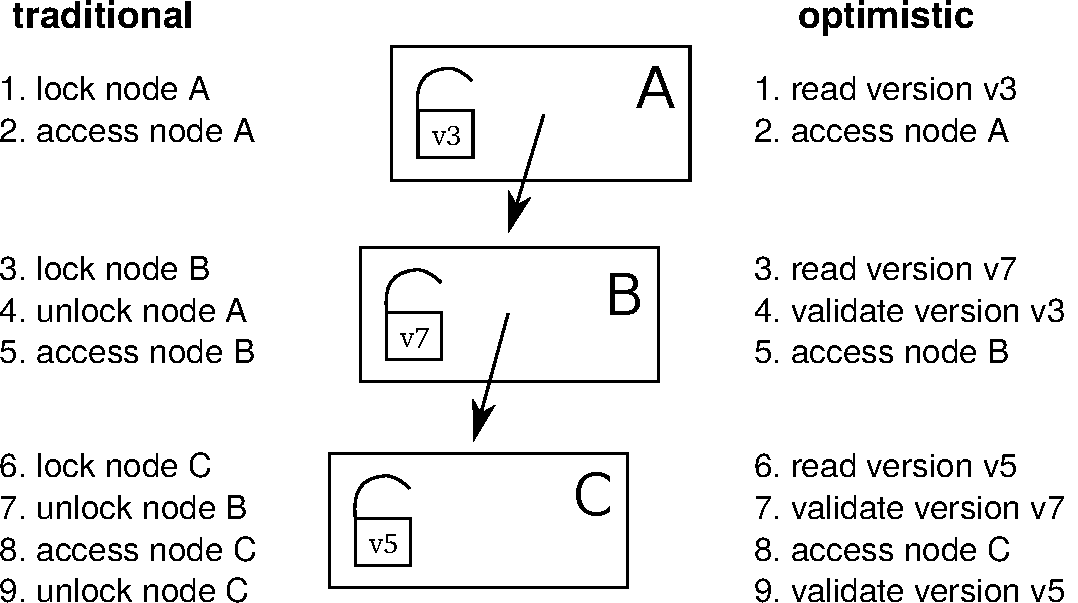
\includegraphics[width=0.65\linewidth]{olcall.pdf}
  \vspace{0.2cm}
  \caption{Comparison of a lookup operation in a 3-level tree using traditional lock coupling (left-hand side) vs.~optimistic lock coupling (right-hand side).}
  \label{fig:olc}
\end{figure}

The traditional and most common lock-based synchronization protocol for B-trees is lock coupling, which interleaves lock acquisitions while holding at most two locks at a time.
If, as we observed earlier, optimistic locks have similar semantics as traditional locks, it is natural to ask whether lock coupling can be combined with optimistic locks.
And indeed the answer is yes: One can almost mechanically translate traditional lock coupling code to optimistic lock coupling code.
This is illustrated in Figure~\ref{fig:olc}, which compares the traversal in a tree of height 3 using traditional and optimistic locks.
As the figure shows, the main difference is that locking is translated to reading the version and that unlocking becomes validation of the previously read version.
This simple change provides efficient lock-free tree traversal without the need to design a complex synchronization protocol.

It is important to emphasize the conceptual simplicity of OLC in comparison to data structures that use custom protocols like the Bw-tree~\cite{DBLP:conf/icde/LevandoskiLS13a}.
To implement lock-free access, the Bw-tree requires an indirection table, delta nodes, complex splitting and merging logic, retry logic, etc.
OLC, on the other hand, can directly be applied to B-trees mostly by adding the appropriate optimistic locking code and without modifying the node layout itself.
Therefore, OpenBw-Tree, an open source implementation of the Bw-tree, requires an order of magnitude more code than a B-tree based on OLC\footnote{Both implementations are available on GitHub: \url{https://github.com/wangziqi2016/index-microbench}}.
Given how difficult it is to develop, validate, and debug lock-free code, simplicity is obviously a major advantage.

\subsection{Correctness Aspects}

\begin{figure}
  % \centering
  %[basicstyle=\normalsize\ttfamily,showstringspaces=false,columns=fullflexible,breaklines=false,breakatwhitespace=true,numbers=none,numberstyle=\small,style=C,keepspaces=true]
\begin{lstlisting}[basicstyle=\ttfamily,language=C++,numbers=left,numberstyle=\small]
std::atomic<BTreeNode*> root;

// search for key in B+tree, returns payload in resultOut
bool lookup(Key key, Value& resultOut) {
   BTreeNode* node = root.load();
   uint64_t nodeVersion = node->readLockOrRestart();
   if (node != root.load()) // make sure the root is still the root
      restart();

   BTreeInner<Key>* parent = nullptr;
   uint64_t parentVersion = 0;

   while (node->isInner()) {
      auto inner = (BTreeInner*)node;

      // unlock parent and make current node the parent
      if (parent)
         parent->readUnlockOrRestart(parentVersion);
      parent = inner;
      parentVersion = nodeVersion;

      // search for next node
      node = inner->findChild(key);
      // validate 'inner' to ensure that 'node' pointer is valid
      inner->checkOrRestart(nodeVersion);
      // now it safe to dereference 'node' pointer (read its version)
      nodeVersion = node->readLockOrRestart();
   }

   // search in leaf and retrieve payload
   auto leaf = (BTreeLeaf*)node;
   bool success = leaf->findValue(key, resultOut);

   // unlock everything
   if (parent)
      parent->readUnlockOrRestart(parentVersion);
   node->readUnlockOrRestart(nodeVersion);

   return success;
}
\end{lstlisting}
  \vspace{0.2cm}
  \caption{B-tree lookup code using OLC. For simplicity, the restart logic is not shown.}
  \label{fig:lookup}
\end{figure}

So far, we have introduced the high-level ideas behind OLC and have stressed its similarity to traditional lock coupling.
Let us now discuss some cases where the close similarity between lock coupling and OLC breaks down.
To make this more concrete, we show the B-tree lookup code in Figure~\ref{fig:lookup}.
In the code, \texttt{readLockOrRestart} reads the lock version and \texttt{readUnlockOrRestart} validates that the read was correct.

One issue with OLC is that any pointer speculatively read from a node may point to invalid memory (if that node is modified concurrently).
Dereferencing such a pointer (e.g., to read its optimistic lock), may cause a segmentation fault or undefined behavior.
In the code shown in Figure~\ref{fig:lookup}, this problem is prevented by the extra check in line 25, which ensures that the read from the node containing the pointer was correct.
Without this additional validation, the code would in line 27 dereference the pointer speculatively read in line 23.
Note that the implementation of \texttt{checkOrRestart} is actually identical to \texttt{readUnlockOrRestart}.
We chose to give it a different name to highlight the fact that this extra check would not be necessary with read/write locks.

Another potential issue with optimistic locks is code that does not terminate.
Code that speculatively accesses a node, like an intra-node binary search, should be written in a way such that it always terminates---even in the presence of concurrent writes.
Otherwise, the validation code that detects the concurrent write will never run.
The binary search of a B-tree, for example, needs to be written in such a way that each comparison makes progress.
For some data structures that do not require loops in the traversal code (like ART) termination is trivially true.

\subsection{Implementation Details}

% implementation, efficiency
To implement an optimistic lock, one can combine the lock and the version counter into a single 64-bit\footnote{Even after subtracting one bit for the lock status, a back-of-the-envelope calculation can show that 63 bits are large enough to never overflow in practice.} word~\cite{artsync}.
A typical read operation will therefore merely consist of reading this version counter atomically.
In C++11 this can be implemented using the \texttt{std::atomic} type.

On x86, atomic reads are cheap because of x86's strong memory order guarantees.
No memory fences are required for sequentially-consistent loads, which are translated (by both GCC and clang) into standard \texttt{MOV} instructions.
Hence, the only effect of \texttt{std::atomic} for loads is preventing instruction re-ordering.
This makes version access and validation cheap.
Acquiring and releasing an optimistic lock in exclusive mode has comparable cost to a traditional lock:
A fairly expensive sequentially-consistent store is needed for acquiring a lock, while a standard \texttt{MOV} suffices for releasing it.
A simple sinlock-based implementation of optimistic locks can be found in the appendix of an earlier paper~\cite{artsync}.

OLC code must be able to handle restarts since validation or lock upgrade can fail due to concurrent writers.
Restarts can easily be implemented by wrapping the data structure operation in a loop (for simplicity not shown in Figure~\ref{fig:lookup}).
Such a loop also enables limiting the number of optimistic retry operations and falling back to pessimistic locking in cases of very heavy contention.
The ability to fall back to traditional locking is a major advantage of OLC in terms of robustness over lock-free approaches, which do not have this option.

In addition to the optimistic shared mode and the exclusive mode, optimistic locks also support a ``shared pessimistic'' mode, which physically acquires the lock in shared mode (allowing multiple concurrent readers but no writers).
This mode is useful for table (or range) scans that touch many tuples on a leaf page (which would otherwise easily abort).
Finally, let us mention that large range scans and table scans, should be broken up into several per-node traversals as is done in the LeanStore~\cite{leanstore} system.

Like all lock-free data structures, but unlike traditional locking and Hardware Transactional Memory~\cite{DBLP:conf/hpca/KarnagelDRLLSL14,DBLP:journals/pvldb/MakreshanskiLS15,htmtkde}, OLC requires care when deleting (and reusing) nodes.
The reason is that a deleting thread can never be sure that a node can be reclaimed because other threads might still be optimistically reading from that node.
Therefore, standard solutions like epoch-based reclamation~\cite{DBLP:conf/sosp/TuZKLM13}, hazard pointers~\cite{DBLP:journals/tpds/Michael04}, or optimized hazard pointers~\cite{DBLP:conf/spaa/BalmauGHZ16} need to be used.
These memory reclamation techniques are, however, largely orthogonal to the synchronization protocol itself.

%-lock-free is not a strong guarantee

\newpage
\section{Evaluation}\label{sec:evaluation}

Let us now experimentally evaluate the overhead and scalability of OLC.
For the experiments, we use an in-memory B+tree implemented in C++11 using templates, which is configured to use nodes of 4096 bytes, random 8 byte keys, and 8 byte payloads.
Based on this B-tree, we compare the following synchronization approaches:
\begin{itemize}
\item an OLC implementation\footnote{An almost identical OLC implementation is available on github: \url{https://github.com/wangziqi2016/index-microbench/tree/master/BTreeOLC}}
\item a variant based on traditional lock coupling and read/write locks
\item the unsynchronized B-tree, which obviously is only correct for read-only workloads but allows measuring the overhead of synchronization
\end{itemize}
Note that earlier work has compared the OLC implementation with a Bw-tree implementation~\cite{buzzword} and other state-of-the-art in-memory index structures.

We use a Haswell EP system with an Intel Xeon E5-2687W v3 CPU, which has 10 cores (20 ``Hyper-Threads'') and 25~MB of L3 cache.
The system is running Ubuntu 18.10 and we use GCC 8.2.0 to compile our code.
The CPU counters are obtained using the Linux perf API\footnote{We use the following convenience wrapper: \url{https://github.com/viktorleis/perfevent}}.

\begin{table}
  \caption{Performance and CPU counters for lookup and insert operations in a B-tree with 100M keys. We perform 100M operations and normalize the CPU counters by that number.}
  \label{tab:overhead}
  \centering
  \begin{tabular}{lrrrrrrr}\toprule
                    &         &        &        & instruc-  & L1     & L3     & branch \\
                    & threads & M op/s & cycles & tions & misses & misses & misses \\\midrule
lookup (no sync.)   & 1       & 1.72   & 2028   & 283     & 39.1   & 14.9   & 16.1   \\
lookup (OLC)        & 1       & 1.65   & 2107   & 370     & 43.9   & 15.1   & 16.7   \\
lookup (lock coup.) & 1       & 1.72   & 2078   & 365     & 42.3   & 16.9   & 15.7   \\\midrule
insert (no sync.)   & 1       & 1.51   & 2286   & 530     & 59.8   & 31.1   & 17.3   \\
insert (OLC)        & 1       & 1.50   & 2303   & 629     & 61.2   & 31.1   & 16.5   \\
insert (lock coup.) & 1       & 1.41   & 2473   & 644     & 61.0   & 31.0   & 17.2   \\\midrule
lookup (no sync.)   & 10      & 15.48  & 2058   & 283     & 38.6   & 15.5   & 16.0   \\
lookup (OLC)        & 10      & 14.60  & 2187   & 370     & 43.8   & 15.8   & 16.8   \\
lookup (lock coup.) & 10      & 5.71   & 5591   & 379     & 54.2   & 17.0   & 14.8   \\\midrule
insert (no sync.)   & 10      & -      & -      & -       & -      & -      & -      \\
insert (OLC)        & 10      & 10.46  & 2940   & 656     & 62.0   & 32.5   & 16.8   \\
insert (lock coup.) & 10      & 7.55   & 4161   & 667     & 75.0   & 28.6   & 16.2   \\
    \bottomrule
\end{tabular}
\end{table}

Table~\ref{tab:overhead} compares the performance and CPU counters for lookup and insert operations in a B-tree with 100M keys.
With {\em single-threaded} execution, we observe that all three approaches have very similar performance.
Adding traditional or optimistic locks to unsynchronized B-tree code results in up to 30\% of additional instructions without affecting single-threaded performance much.

\begin{figure}
  \centering
  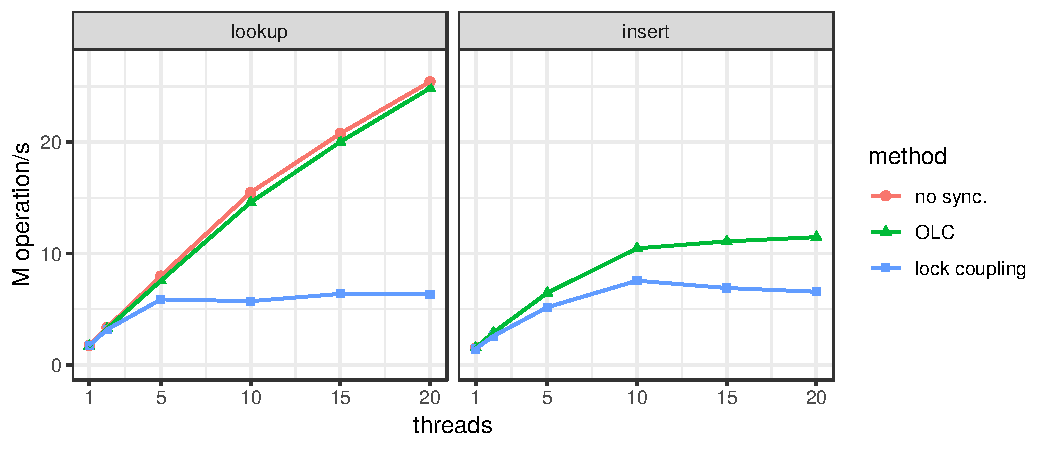
\includegraphics[width=\linewidth]{scale.pdf}
  \vspace{0.2cm}
  \caption{Scalability on 10-core system for B-tree operations (100M values).}
  \label{fig:scale}
\end{figure}

As Figure~\ref{fig:scale} shows, the results change dramatically once we use multiple threads.
For lookup, the scalability of OLC is near-linear up to 20 threads, even though the system has only 10 ``real cores''.
The OLC scalability for insert is also respectable (though not quite as linear because multi-threaded insertion approaches the memory bandwidth of our processor).
The figure also shows that the results of traditional lock coupling with read/write locks are significantly worse than OLC.
With 20 threads, lookup with OLC is 3.9$\times$ faster than traditional lock coupling.

\section{Summary}\label{sec:conc}

Optimistic Lock Coupling (OLC) is an effective synchronization method that combines the simplicity of traditional lock coupling with the superior scalability of lock-free approaches.
OLC is widely applicable and has already been successfully used to synchronize several data structures, including B-trees, binary search trees, and different trie variants.
These features make it highly attractive for modern database systems as well as performance-critical systems software in general.

\begin{thebibliography}{10}

\bibitem{DBLP:conf/spaa/BalmauGHZ16}
O.~Balmau, R.~Guerraoui, M.~Herlihy, and I.~Zablotchi.
\newblock Fast and robust memory reclamation for concurrent data structures.
\newblock In {\em SPAA}, 2016.

\bibitem{DBLP:journals/acta/BayerS77}
R.~Bayer and M.~Schkolnick.
\newblock Concurrency of operations on {B}-trees.
\newblock {\em Acta Informatica}, 9, 1977.

\bibitem{hot}
R.~Binna, E.~Zangerle, M.~Pichl, G.~Specht, and V.~Leis.
\newblock {HOT}: A height optimized trie index for main-memory database
  systems.
\newblock In {\em SIGMOD}, 2018.

\bibitem{DBLP:conf/ppopp/BronsonCCO10}
N.~G. Bronson, J.~Casper, H.~Chafi, and K.~Olukotun.
\newblock A practical concurrent binary search tree.
\newblock In {\em PPOPP}, 2010.

\bibitem{DBLP:conf/vldb/ChaHKK01}
S.~K. Cha, S.~Hwang, K.~Kim, and K.~Kwon.
\newblock Cache-conscious concurrency control of main-memory indexes on
  shared-memory multiprocessor systems.
\newblock In {\em VLDB}, 2001.

\bibitem{intel}
I.~Cutress.
\newblock {Intel} goes for 48-cores: {Cascade-AP} with multi-chip package
  coming soon.
\newblock
  \url{https://www.anandtech.com/show/13535/intel-goes-for-48cores-cascade-ap},
  2018 (accessed January, 2019).

\bibitem{DBLP:conf/cidr/FaleiroA17}
J.~M. Faleiro and D.~J. Abadi.
\newblock Latch-free synchronization in database systems: Silver bullet or
  fool's gold?
\newblock In {\em CIDR}, 2017.

\bibitem{DBLP:journals/ftdb/Graefe11}
G.~Graefe.
\newblock Modern {B}-tree techniques.
\newblock {\em Foundations and Trends in Databases}, 3(4), 2011.

\bibitem{DBLP:conf/hpca/KarnagelDRLLSL14}
T.~Karnagel, R.~Dementiev, R.~Rajwar, K.~Lai, T.~Legler, B.~Schlegel, and
  W.~Lehner.
\newblock Improving in-memory database index performance with
  {Intel}\({}^{\mbox{{\textregistered}}}\) transactional synchronization
  extensions.
\newblock In {\em HPCA}, 2014.

\bibitem{DBLP:journals/tods/LehmanY81}
P.~L. Lehman and S.~B. Yao.
\newblock Efficient locking for concurrent operations on {B}-trees.
\newblock {\em {ACM} Trans. Database Syst.}, 6(4), 1981.

\bibitem{leanstore}
V.~Leis, M.~Haubenschild, A.~Kemper, and T.~Neumann.
\newblock Leanstore: In-memory data management beyond main memory.
\newblock In {\em ICDE}, 2018.

\bibitem{art}
V.~Leis, A.~Kemper, and T.~Neumann.
\newblock The adaptive radix tree: {ARTful} indexing for main-memory databases.
\newblock In {\em ICDE}, 2013.

\bibitem{htmtkde}
V.~Leis, A.~Kemper, and T.~Neumann.
\newblock Scaling {HTM}-supported database transactions to many cores.
\newblock {\em {IEEE} Trans. Knowl. Data Eng.}, 28(2), 2016.

\bibitem{artsync}
V.~Leis, F.~Scheibner, A.~Kemper, and T.~Neumann.
\newblock The {ART} of practical synchronization.
\newblock In {\em DaMoN}, 2016.

\bibitem{DBLP:conf/icde/LevandoskiLS13a}
J.~J. Levandoski, D.~B. Lomet, and S.~Sengupta.
\newblock The {Bw}-tree: A {B}-tree for new hardware platforms.
\newblock In {\em ICDE}, 2013.

\bibitem{DBLP:journals/pvldb/MakreshanskiLS15}
D.~Makreshanski, J.~J. Levandoski, and R.~Stutsman.
\newblock To lock, swap, or elide: On the interplay of hardware transactional
  memory and lock-free indexing.
\newblock {\em {PVLDB}}, 8(11), 2015.

\bibitem{DBLP:dblp_conf/eurosys/MaoKM12}
Y.~Mao, E.~Kohler, and R.~T. Morris.
\newblock Cache craftiness for fast multicore key-value storage.
\newblock In {\em EuroSys}, 2012.

\bibitem{DBLP:journals/tpds/Michael04}
M.~M. Michael.
\newblock Hazard pointers: Safe memory reclamation for lock-free objects.
\newblock {\em {IEEE} Trans. Parallel Distrib. Syst.}, 15(6), 2004.

\bibitem{DBLP:journals/jacm/ShalevS06}
O.~Shalev and N.~Shavit.
\newblock Split-ordered lists: Lock-free extensible hash tables.
\newblock {\em J. {ACM}}, 53(3), 2006.

\bibitem{amd}
A.~Shilov.
\newblock {AMD} previews {EPYC} ‘{Rome}’ processor: Up to 64 {Zen} 2 cores.
\newblock
  \url{https://www.anandtech.com/show/13561/amd-previews-epyc-rome-processor-up-to-64-zen-2-cores},
  2018 (accessed January, 2019).

\bibitem{DBLP:conf/sosp/TuZKLM13}
S.~Tu, W.~Zheng, E.~Kohler, B.~Liskov, and S.~Madden.
\newblock Speedy transactions in multicore in-memory databases.
\newblock In {\em SOSP}, 2013.

\bibitem{buzzword}
Z.~Wang, A.~Pavlo, H.~Lim, V.~Leis, H.~Zhang, M.~Kaminsky, and D.~Andersen.
\newblock Building a {Bw}-tree takes more than just buzz words.
\newblock In {\em SIGMOD}, 2018.

\end{thebibliography}


%\bibliographystyle{abbrv}
%\bibliography{main}

\end{document}

\end{article}


\begin{article}
{Accelerating the Machine Learning Lifecycle with {MLflow}}
{Matei Zaharia, Andrew Chen, Aaron Davidson, Ali Ghodsi, Sue Ann Hong, Andy Konwinski, Siddharth Murching, Tomas Nykodym, Paul Ogilvie, Mani Parkhe, Fen Xie, Corey Zumar}
\graphicspath{{submissions/mlflow/}}
\documentclass[11pt]{article}
%\documentclass[11pt,dvipdfm]{article}

\usepackage{deauthor}
\usepackage{url}            % simple URL typesetting
\usepackage{graphicx}
\usepackage{times}
\usepackage{fancyvrb}
\usepackage{comment}

% \graphicspath{{authorname/}}

\begin{document}

%\title{MLflow: An Open Platform for Machine Learning Experimentation, Reproducibility and Production}
%\title{MLflow: An Open Platform for the End-to-End Machine Learning Lifecycle}
\title{Accelerating the Machine Learning Lifecycle with {MLflow}}

% The \author macro works with any number of authors. There are two
% commands used to separate the names and addresses of multiple
% authors: \And and \AND.
%
% Using \And between authors leaves it to LaTeX to determine where to
% break the lines. Using \AND forces a line break at that point. So,
% if LaTeX puts 3 of 4 authors names on the first line, and the last
% on the second line, try using \AND instead of \And before the third
% author name.

\author{
  \textbf{Matei Zaharia, Andrew Chen, Aaron Davidson, Ali Ghodsi, Sue Ann Hong, Andy Konwinski,}\\
  \textbf{Siddharth Murching, Tomas Nykodym, Paul Ogilvie, Mani Parkhe, Fen Xie, Corey Zumar} \\
  Databricks Inc.\\
  %% examples of more authors
  %% \And
  %% Coauthor \\
  %% Affiliation \\
  %% Address \\
  %% \texttt{email} \\
  %% \AND
  %% Coauthor \\
  %% Affiliation \\
  %% Address \\
  %% \texttt{email} \\
  %% \And
  %% Coauthor \\
  %% Affiliation \\
  %% Address \\
  %% \texttt{email} \\
  %% \And
  %% Coauthor \\
  %% Affiliation \\
  %% Address \\
  %% \texttt{email} \\
}

\maketitle

\begin{abstract}
Machine learning development creates multiple new challenges that are not present in a traditional software development lifecycle.
These include keeping track of the myriad inputs to an ML application (e.g., data versions, code and tuning parameters), reproducing results, and production deployment.
In this paper, we summarize these challenges from our experience with Databricks customers, and describe MLflow, an open source platform we recently launched to streamline the machine learning lifecycle.
MLflow covers three key challenges: experimentation, reproducibility, and model deployment, using generic APIs that work with any ML library, algorithm and programming language.
The project has a rapidly growing open source community, with over 50 contributors since its launch in June 2018.
\end{abstract}

\section{Introduction}

Machine learning development requires solving new problems that are not part of the standard software development lifecycle.
For example, while traditional software has a well-defined set of product features to be built, ML development tends to revolve around \emph{experimentation}: the ML developer will constantly experiment with new datasets, models, software libraries, tuning parameters, etc.~to optimize a business metric such as model accuracy.
Because model performance depends heavily on the input data and training process, \emph{reproducibility} is paramount throughout ML development.
Finally, in order to have business impact, ML applications need to be \emph{deployed} to production, which means both deploying a model in a way that can be used for inference (e.g., REST serving) and deploying scheduled jobs to regularly update the model.
This is especially challenging when deployment requires collaboration with another team, such as application engineers who are not ML experts.

Based on our conversations with dozens of Databricks customers that use machine learning, these lifecycle problems are a major bottleneck in practice.
Although today's ML libraries provide tools for part of the lifecycle, there are no standard systems and interfaces to manage the full process.
For example, TensorFlow offers a training API and a Serving system~\cite{tfx}, but TensorFlow Serving cannot easily be used for models from another ML library, or from an incompatible version of TensorFlow.
In practice, an organization will need to run models from multiple ML libraries, TensorFlow versions, etc., and has to design its own infrastructure for this task.


Faced with these challenges, many organizations try to ``lock down'' the ML development process to obtain reproducibility and deployability.
Some organizations develop internal guidelines for ML development, such as which libraries one can use that the production team will support.
Others develop internal \emph{ML platforms} (e.g., Facebook's FBLearner~\cite{fblearner}, Uber's Michelangelo~\cite{michelangelo} and Google's TFX~\cite{tfx}): APIs that ML developers must use in order to build deployable models.
Unfortunately, both approaches limit ML developers in the algorithms and libraries they can use, decreasing their ability to experiment, and both create substantial engineering work whenever the ML developers want to use new libraries or models.

%Some organizations ask each ML team to manage its own infrastructure, which is expensive.
%Others try to develop shared \emph{ML platforms} that data scientists must use to build their models (e.g., Facebook's FBLearner~\cite{fblearner} and Uber's Michelangelo~\cite{michelangelo}), but this approach also has challenges, because model developers are limited to the algorithms and libraries supported by the platform and cannot easily experiment with others.

In this paper, we summarize our experience with ML lifecycle challenges at Databricks customers and describe MLflow, an open source ML platform we are developing to address these challenges.
MLflow's key principle is an \emph{open interface} design, where data scientists and engineers can bring their own training code, metrics, and inference logic while benefitting from a structured development process.
%MLflow leverages simple, generic interfaces such as Docker containers and REST APIs to achieve this goal.
For example, a ``model'' saved in MLflow can simply be a Python function (and associated library dependencies) that MLflow then knows how to deploy in various environments (e.g., batch or real-time scoring).
Other MLflow abstractions are likewise based on generic interfaces, such as REST APIs and Docker containers.
Compared to existing ML platforms like FBLearner, Michelangelo and TFX, this open interface design gives users flexibility and control while retaining the benefits of lifecycle management.
%Moreover, MLflow's open source nature enables easily sharing ML work across organizations.
The current version of MLflow provides APIs for experiment tracking, reproducible runs and model packaging and deployment, usable in Python, Java and R.
We describe these APIs and some sample MLflow use cases to show how the system can streamline the machine learning lifecycle.

\section{Challenges in Machine Learning Development}

ML faces many of the challenges in traditional software development, such as testing, code review, monitoring, etc.
In other ways, however, ML applications are different from traditional software, and present new problems.

One of the main differences is that the goal in machine learning is to \emph{optimize} a specific metric, such as prediction accuracy, instead of simply meeting a set of functional requirements.
For example, for a retailer, every 1\% improvement in prediction accuracy for a recommendation engine might lead to millions of dollars in revenue, so the ML team working on this engine will continuously want to improve the model.
This means that ML developers wish to continuously experiment with the latest models, software libraries, etc.,~to improve target metrics.
Beyond this difference in objective, ML applications are more complex to manage because their performance depends on training data, tuning, and concerns such as overfitting that do not occur in other applications.
%This means that reproducibility of these runtime conditions is important.
Finally, ML applications are often developed by teams or individuals with very different expertise, and hand-off between these individuals can be challenging.
For example, a data scientist might be an expert at ML training, and use her skills to create a model, but she might need to pass the model to a software engineer for deployment within an application.
Any errors in this process (e.g., mismatched software versions or data formats) might lead to incorrect results that are hard for a software engineer without ML knowledge to debug.

Based on these requirements in working with ML, we found four challenges to arise repeatedly at ML users:

\vspace{-0.6em}
\paragraph{1. Multitude of tools.} Hundreds of software tools cover each phase of ML development, from data preparation to model training to deployment. However, unlike traditional software development, where teams select \emph{one} tool for each phase, ML developers usually want to try \emph{every} available tool (e.g., algorithm) to see whether it improves results. For example, a team might try multiple preprocessing libraries (e.g., Pandas and Apache Spark) to featurize data; multiple model types (e.g. trees and deep learning); and even multiple frameworks for the same model type (e.g., TensorFlow and PyTorch) to run various models published online by researchers. %This diversity of tools means that ML teams need to use and productionize dozens of libraries.

\vspace{-0.6em}
\paragraph{2. Experiment tracking.} Machine learning results are affected by dozens of configurable parameters, ranging from the input data to hyperparameters and preprocessing code. Whether an individual is working alone or on a team, it is difficult to track which parameters, code, and data went into each experiment to produce a model.

\vspace{-0.6em}
\paragraph{3. Reproducibility.} Without detailed tracking, teams often have trouble getting the same code to work again. For example, a data scientist passing her training code to an engineer for use in production might see problems if the engineer modifies it, and even a user working alone needs to reliably reproduce old results to stay productive. %Even ML researchers frequently experience this problem when trying to reproduce published work.

\vspace{-0.6em}
\paragraph{4. Production deployment.} Moving an application to production can be challenging, both for inference and training. First, there are a plethora of possible inference environments, such as REST serving, batch scoring and mobile applications, but there is no standard way to move models from any library to these diverse environments. Second, the model training pipeline also needs to be reliably converted to a scheduled job, which requires care to reproduce the software environments, parameters, etc.~used in development.
Production deployment is especially challenging because it often requires passing the ML application to a different team with less ML expertise.

~

\vspace{-0.6em}
To address these problems, we believe that ML development processes should be explicitly designed to promote reproducibility, deployability, etc. The challenge is how to do so while leaving maximum flexibility for ML developers to build the best possible model. This led us to the open interface design philosophy for MLflow.

\section{MLflow Overview}

To structure the ML development process while leaving users maximum flexibility, we built MLflow around an \emph{open interface} philosophy: the system should define general interfaces for each abstraction (e.g., a training step, a deployment tool or a model) that allow users to bring their own code or workflows.
For example, many existing ML tools represent models using a serialization format, such as TensorFlow graphs~\cite{abadi2016tensorflow}, ONNX~\cite{onnx} or PMML~\cite{pmml}, when passing them from training to serving. This restricts applications to using specific libraries.
In contrast, in MLflow, a model can be represented simply as a Python function (and library dependency information), so any development tool that knows how to run a Python function can run such a model.
For more specialized deployment tools, a model can also expose other interfaces called ``flavors" (e.g., an ONNX graph) while still remaining viewable as just a Python function.
As another example, MLflow exposes most of its features through REST APIs that can called from any programming language.

More specifically, MLflow provides three components, which can either be used together or separately:

\begin{itemize}
\item \textbf{MLflow Tracking}, which is an API for recording experiment runs, including code used, parameters, input data, metrics, and arbitrary output files. These runs can then be queried through an API or UI.

\item\textbf{MLflow Projects}, a simple format for packaging code into reusable projects. Each project defines its environment (e.g., software libraries required), the code to run, and parameters that can be used to call the project programmatically in a multi-step workflow or in automated tools such as hyperparameter tuners.

\item\textbf{MLflow Models}, a generic format for packaging models (both the code and data required) that can work with diverse deployment tools (e.g., batch and real-time inference). %The goal is to give users of the model (e.g., a production engineer) a consistent interface for working with models built in different tools.
\end{itemize}

%We next sketch these components in turn; full documentation on them is available at \url{mlflow.org}.

\subsection{MLflow Tracking}

MLflow Tracking is an API for logging and querying \emph{experiment runs}, which consist of parameters, code versions, metrics and arbitrary output files called \emph{artifacts}. Users can start/end runs and log metrics, parameters and artifacts using simple API calls, as shown below using MLflow's Python API:

\begin{Verbatim}[frame=single,fontsize=\small,samepage=true]
# Log parameters, which are arbitrary key-value pairs
mlflow.log_param("num_dimensions", 8)
mlflow.log_param("regularization", 0.1)

# Log metrics; each metric can also be updated throughout the run
mlflow.log_metric("accuracy", 0.8)
mlflow.log_metric("r2", 0.4)

# Log artifacts (arbitrary output files)
mlflow.log_artifact("precision_recall.png")
\end{Verbatim}

MLflow Tracking API calls can be inserted anywhere users run code (e.g., standalone applications or Jupyter notebooks running in the cloud). The tracking API logs results to a local directory by default, but it can also be configured to log over the network to a server, allowing teams to share a centralized MLflow tracking server and compare results from multiple developers.

Once users have recorded runs, MLflow allows users to query them through an API or web-based UI (Figure~\ref{fig:tracking-ui}). This UI includes the ability to organize runs into groups called Experiments, search and sort them, and compare groups of runs, enabling users to build a custom leaderboard for each of their ML problems and even compare results across teams. The UI is inspired by experiment visualization tools such as Sacred~\cite{sacred}, ModelDB~\cite{modeldb} and TensorBoard~\cite{tensorboard}, and supports similar visualizations and queries.

\begin{figure}[h]
\centering
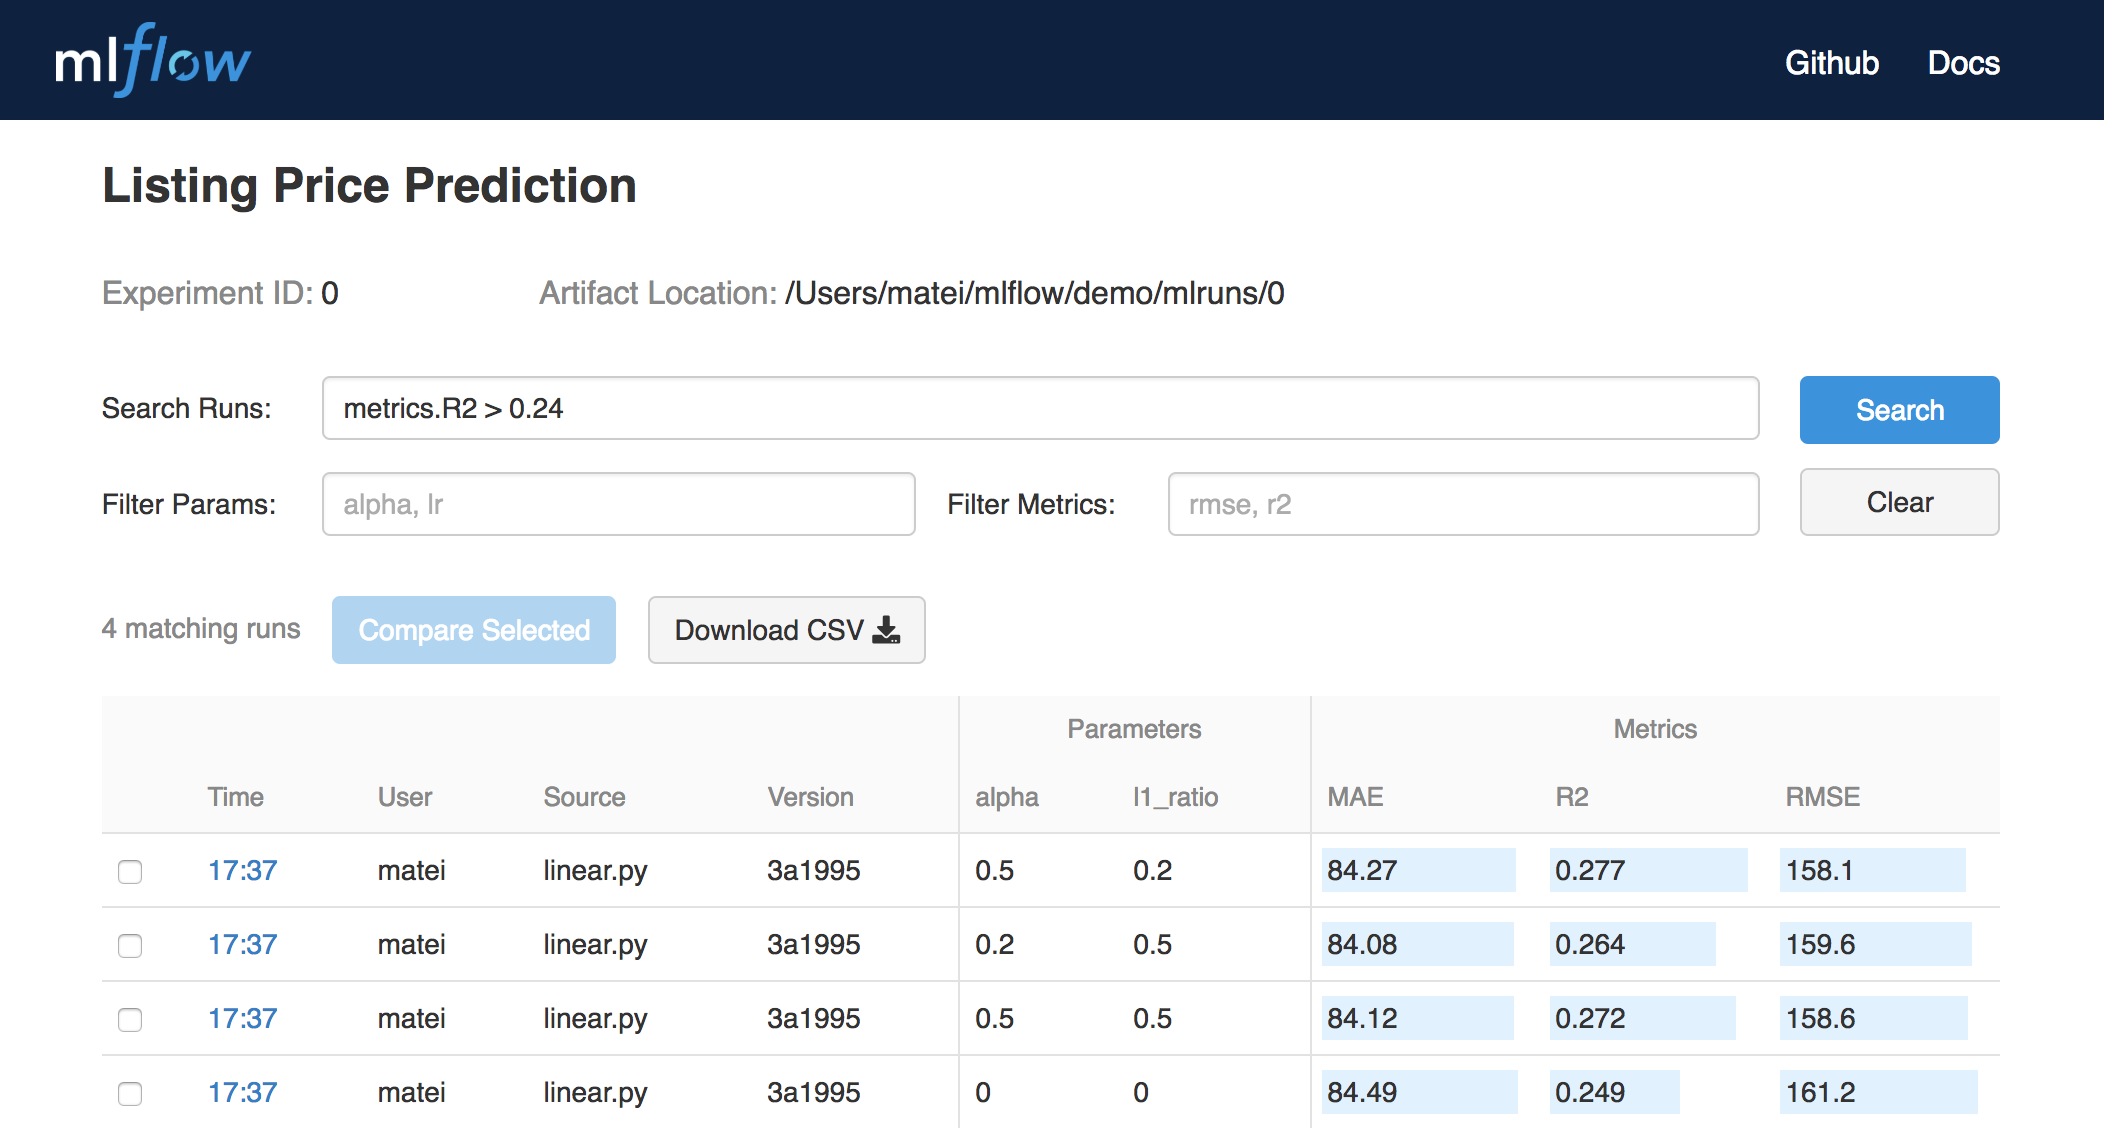
\includegraphics[bb=0 0 1052 564,width=\textwidth]{tracking.png}
\caption{MLflow Tracking UI showing several runs in an experiment. Clicking each run lists its metrics, artifacts and output details and lets the user post comments about the run.}
\label{fig:tracking-ui}
\end{figure}

\subsection{MLflow Projects}

MLflow Projects provide a simple format for packaging reproducible data science code. Each project is simply a directory with code or a Git repository, and uses a descriptor file to specify its dependencies and how to run the code. A MLflow Project is defined by a simple YAML file called MLproject, as shown below:

\begin{Verbatim}[frame=single,fontsize=\small,samepage=true]
name: My Project
conda_env: conda.yaml
entry_points:
  main:
    parameters:
      data_file: path
      alpha: {type: float, default: 0.1}
    command: "python train.py --reg-param {alpha} --data {data_file}"
\end{Verbatim}


Projects can specify their dependencies through a Conda environment or (in an upcoming release) a Docker container specification. A project may also have multiple entry points for invoking runs, with named parameters that downstream users can provide without understanding the internals of the project.

Users can run projects using the \texttt{mlflow run} command line tool, either from local files or a Git repository:

\begin{Verbatim}[frame=single,fontsize=\small,samepage=true]
mlflow run git@github.com:databricks/mlflow-example.git -P alpha=0.5
\end{Verbatim}

Alternatively, projects can be called programmatically using MLflow's API. This can be used to implement multi-step workflows or to pass projects a ``black box'' into automated tools such as hyperparameter search~\cite{hyperopt}.

In either case, MLflow will automatically set up the project's runtime environment and execute it. If the code inside the project uses the MLflow Tracking API, MLflow will also remember the project version executed (that is, the Git commit) and show an \texttt{mlflow run} command to re-execute it in its UI. Finally, MLflow projects can also be submitted to cloud platforms such as Databricks for remote execution.

\subsection{MLflow Models}

MLflow Models are a convention for packaging machine learning models in multiple formats called ``flavors'', allowing diverse tools to understand the model at different levels of abstractions. MLflow also offers a variety of built-in tools to deploy models in its standard favors. For example, the same model can be deployed as a Docker container for REST serving, as an Apache Spark user-defined function (UDF) for batch inference, or into cloud-managed serving platforms like Amazon SageMaker and Azure ML.

Each MLflow Model is simply stored as a directory containing arbitrary files and an MLmodel YAML file that lists the flavors it can be used in and additional metadata about how it was created:

\begin{Verbatim}[frame=single,fontsize=\small,samepage=true]
time_created: 2018-02-21T13:21:34.12
run_id: c4b65fc2c57f4b6d80c6e58a9dcb9f01
flavors:
  sklearn:
    sklearn_version: 0.19.1
    pickled_model: model.pkl
  python_function:
    loader_module: mlflow.sklearn
    pickled_model: model.pkl
\end{Verbatim}

In this example, the model can be used with tools that support either the \texttt{sklearn} or \texttt{python\_function} model flavors. For example, the MLflow SciKit-Learn library knows how to load a \texttt{sklearn} model as a SciKit-Learn Python object, but other deployment tools, such as running the model in a Docker HTTP server, only understand lower-level flavors like \texttt{python\_function}.
In addition, models logged using MLflow Tracking APIs will automatically include a reference to that run's unique ID, letting users discover how they were built.

\section{Example Use Cases}

In this section, we describe three sample MLflow use cases to highlight how users can leverage each component.

\vspace{-0.6em}
\paragraph{Experiment tracking.} A European energy company is using MLflow to track and update hundreds of energy grid models. This team's goal is to build a time series model for every major energy producer (e.g., power plant) and consumer (e.g., factory), monitor these using standard metrics, and combine the predictions to drive business processes such as pricing. Because a single team is responsible for hundreds of models, possibly using different ML libraries, it was important to have a standard development and tracking process. The team has standardized on using Jupyter notebooks for development, MLflow Tracking for metrics, and Databricks jobs for inference.

\vspace{-0.6em}
\paragraph{Reproducible projects.} An online marketplace is using MLflow Projects to package deep learning jobs using Keras and run them in the cloud. Each data scientist develops models locally on his or her laptop using a small dataset, checks them into a Git repository with an MLproject file, and submits remote runs of the project to GPU instances in the cloud for large-scale training or hyperparameter search. Using MLflow Projects makes it easy to create the same software environment in the cloud and share project code between different data scientists.

\vspace{-0.6em}
\paragraph{Model packaging.} The data science team at an e-commerce site is using MLflow Models to package recommendation models for use by application engineers. The technical challenge here was that the recommendation application includes both a standard, ``off-the-shelf'' recommendation model and custom business logic for pre- and post-processing. For example, the application might include custom code to make sure that the recommended items are diverse. This business logic needs to change in sync with the model, and the data science team wants to control both the business logic and the model, without having to submit a patch to the web application each time this logic has to change.
Moreover, the team wants to A/B test distinct models with distinct versions of the processing logic.
The solution was to package both the recommendation model and the custom logic using the \texttt{python\_function} flavor in an MLflow Model, which can then be deployed and tested as a single unit. %This allows production engineers to deploy the recommendation code as they please without the processing logic falling out of sync with the model.

\section{Related Work}

Many software systems aim to simplify ML development.
The closest to our work are the end-to-end ``ML platforms'' at large web companies.
For example, Facebook's FBLearner lets users write reusable workflow steps that run over data in Apache Hive~\cite{fblearner};
Uber's Michelangelo gives users a toolkit of algorithms to choose from that it can automatically train and deploy~\cite{michelangelo}; and Google's TFX provides data preparation and serving tools around TensorFlow~\cite{tfx}.
Anecdotally, these platforms greatly accelerate ML development, showing the benefits of standardizing the ML lifecycle.
However, they generally restrict users to a specific set of algorithms or libraries, so teams are on their own when they step outside these boundaries.
Our goal in MLflow is to let users easily bring their own tools and software in as many steps in the process as possible through our ``open interface'' design.
This includes custom training steps, inference code, and logged parameters and artifacts.

Other systems also tackle specific problems within the ML lifecycle. For example, Sacred~\cite{sacred}, ModelDB~\cite{modeldb} and TensorBoard~\cite{tensorboard} let users track experiments; PMML~\cite{pmml} and ONNX~\cite{onnx} are cross-library model serialization formats; Clipper~\cite{clipper} can deploy arbitrary models as Docker containers; and CDE~\cite{cde}, CodaLab~\cite{codalab}, Binder~\cite{binder} and Repo2Docker~\cite{repo2docker} enable reproducible software runs. MLflow combines these concepts with new ones, such as multi-flavor model packaging, into a unified system design and API.

\section{Conclusion}

For machine learning to have widespread commercial impact, organizations require the same kinds of reliable engineering processes around ML that exist in other engineering disciplines such as software development. In this paper, we have described some of the key challenges that differentiate ML development from traditional software development, such as experimentation, reproducibility, and reliable production deployment. We have also described MLflow, a software platform that can structure the machine learning lifecycle while giving users broad flexibility to use their own ML algorithms, software libraries and development processes.
MLflow is available as open source software at \url{https://www.mlflow.org}.


{\small

\begin{thebibliography}{10}

  \bibitem{abadi2016tensorflow}
  M.~Abadi, P.~Barham, J.~Chen, Z.~Chen, A.~Davis, J.~Dean, M.~Devin,
    S.~Ghemawat, G.~Irving, M.~Isard, et~al.
  \newblock {TensorFlow: A System for Large-Scale Machine Learning}.
  \newblock In {\em OSDI}, volume~16, pages 265--283, 2016.

  \bibitem{tfx}
  D.~Baylor, E.~Breck, H.-T. Cheng, N.~Fiedel, C.~Y. Foo, Z.~Haque, S.~Haykal,
    M.~Ispir, V.~Jain, L.~Koc, C.~Y. Koo, L.~Lew, C.~Mewald, A.~N. Modi,
    N.~Polyzotis, S.~Ramesh, S.~Roy, S.~E. Whang, M.~Wicke, J.~Wilkiewicz,
    X.~Zhang, and M.~Zinkevich.
  \newblock Tfx: A tensorflow-based production-scale machine learning platform.
  \newblock In {\em Proceedings of the 23rd ACM SIGKDD International Conference
    on Knowledge Discovery and Data Mining}, KDD '17, pages 1387--1395, New York,
    NY, USA, 2017. ACM.

  \bibitem{hyperopt}
  J.~Bergstra, B.~Komer, C.~Eliasmith, D.~Yamins, and D.~D. Cox.
  \newblock Hyperopt: a python library for model selection and hyperparameter
    optimization.
  \newblock {\em Computational Science and Discovery}, 8(1):014008, 2015.

  \bibitem{binder}
  {Binder}.
  \newblock \url{https://mybinder.org}, 2018.

  \bibitem{clipper}
  D.~Crankshaw, X.~Wang, G.~Zhou, M.~J. Franklin, J.~E. Gonzalez, and I.~Stoica.
  \newblock Clipper: A low-latency online prediction serving system.
  \newblock In {\em Proceedings of the 14th USENIX Conference on Networked
    Systems Design and Implementation}, NSDI'17, pages 613--627, Berkeley, CA,
    USA, 2017. USENIX Association.

  \bibitem{fblearner}
  J.~Dunn.
  \newblock Introducing {FBLearner Flow}: Facebook’s {AI} backbone.
  \newblock
    \url{https://code.fb.com/core-data/introducing-fblearner-flow-facebook-s-ai-backbone/}.

  \bibitem{repo2docker}
  J.~Forde, T.~Head, C.~Holdgraf, Y.~Panda, G.~Nalvarte, M.~Pacer, F.~Perez,
    B.~Ragan-Kelley, and E.~Sundell.
  \newblock Reproducible research environments with repo2docker.
  \newblock ICML, 07/2018 2018.

  \bibitem{tensorboard}
  Google.
  \newblock Tensorboard: Visualizing learning.
  \newblock \url{https://www.tensorflow.org/guide/summaries_and_tensorboard}.

  \bibitem{pmml}
  A.~Guazzelli, W.-C. Lin, and T.~Jena.
  \newblock {\em PMML in Action: Unleashing the Power of Open Standards for Data
    Mining and Predictive Analytics}.
  \newblock CreateSpace, Paramount, CA, 2nd edition, 2012.

  \bibitem{cde}
  P.~J. Guo.
  \newblock {CDE}: A tool for creating portable experimental software packages.
  \newblock {\em Computing in Science and Engineering}, 14(4):32--35, 2012.

  \bibitem{michelangelo}
  J.~Hermann and M.~D. Balso.
  \newblock Meet {Michelangelo}: Uber’s machine learning platform.
  \newblock \url{https://eng.uber.com/michelangelo/}.

  \bibitem{sacred}
  {K}laus {G}reff, {A}aron {K}lein, {M}artin {C}hovanec, {F}rank {H}utter, and
    {J}\"urgen {S}chmidhuber.
  \newblock {T}he {S}acred {I}nfrastructure for {C}omputational {R}esearch.
  \newblock In {K}aty {H}uff, {D}avid {L}ippa, {D}illon {N}iederhut, and
    M.~{P}acer, editors, {\em {P}roceedings of the 16th {P}ython in {S}cience
    {C}onference}, pages 49 -- 56, 2017.

  \bibitem{codalab}
  P.~Liang et~al.
  \newblock {CodaLab}.
  \newblock \url{https://worksheets.codalab.org}, 2018.

  \bibitem{onnx}
  {ONNX Group}.
  \newblock {ONNX}.
  \newblock \url{https://onnx.ai}.

  \bibitem{modeldb}
  M.~Vartak, H.~Subramanyam, W.-E. Lee, S.~Viswanathan, S.~Husnoo, S.~Madden, and
    M.~Zaharia.
  \newblock Modeldb: A system for machine learning model management.
  \newblock In {\em Proceedings of the Workshop on Human-In-the-Loop Data
    Analytics}, HILDA '16, pages 14:1--14:3, New York, NY, USA, 2016. ACM.

  \end{thebibliography}


}
%\bibliographystyle{abbrv}
%\bibliography{paper}

\end{document}

\end{article}



\begin{article}
{From the Edge to the Cloud: Model Serving in ML.NET}
{Yunseong Lee, Alberto Scolari, Byung-Gon Chun, Markus Weimer, Matteo Interlandi}
\graphicspath{{submissions/model_serving_dot_net/figs/}}
\pdfminorversion=5
\documentclass[11pt]{article}
\usepackage{deauthor,times,graphicx,caption,microtype}
\usepackage{hyperref}
\usepackage{listings}
\usepackage{booktabs}

\begin{document}

\title{Optimistic Lock Coupling: A Scalable and Efficient General-Purpose Synchronization Method}

\author{Viktor Leis, Michael Haubenschild\raisebox{0.9ex}{$\ast$}, Thomas Neumann\\ Technische Universit{\"a}t M{\"u}nchen \hspace{0.7cm} Tableau Software\raisebox{0.9ex}{$\ast$} \\ {\{leis,neumann\}{@}in.tum.de} \hspace{0.7cm} {mhaubenschild{@}tableau.com\raisebox{0.9ex}{$\ast$}}}

\maketitle

\begin{abstract}
As the number of cores on commodity processors continues to increase, scalability becomes more and more crucial for overall performance.
Scalable and efficient concurrent data structures are particularly important, as these are often the building blocks of parallel algorithms.
Unfortunately, traditional synchronization techniques based on fine-grained locking have been shown to be unscalable on modern multi-core CPUs.
Lock-free data structures, on the other hand, are extremely difficult to design and often incur significant overhead.

In this work, we make the case for Optimistic Lock Coupling as a practical alternative to both traditional locking and the lock-free approach.
We show that Optimistic Lock Coupling is highly scalable and almost as simple to implement as traditional lock coupling.
Another important advantage is that it is easily applicable to most tree-like data structures.
We therefore argue that Optimistic Lock Coupling, rather than a complex and error-prone custom synchronization protocol, should be the default choice for performance-critical data structures.
\end{abstract}

\section{Introduction}

% more and more cores
Today, Intel's commodity server processors have up to 28 cores and its upcoming microarchitecture will have up to 48 cores per socket~\cite{intel}.
Similarly, AMD currently stands at 32 cores and this number is expected to double in the next generation~\cite{amd}.
Since both platforms support simultaneous multithreading (also known as hyperthreading), affordable commodity servers (with up to two sockets) will soon routinely have between 100 and 200 hardware threads.

% data structure scalability is important
With such a high degree of hardware parallelism, efficient data processing crucially depends on how well concurrent data structures scale.
Internally, database systems use a plethora of data structures like table heaps, internal work queues, and, most importantly, index structures.
Any of these can easily become a scalability (and therefore overall performance) bottleneck on many-core CPUs.

% traditional synchronization: fine-grained locks, slow, cache invalidation
Traditionally, database systems synchronize internal data structures using fine-grained reader/writer locks\footnote{In this work, we focus on data structure synchronization rather than high-level transaction semantics and therefore use the term {\em lock} for what would typically be called {\em latch} in the database literature. We thus follow common computer science (rather than database) terminology.}.
Unfortunately, while fine-grained locking makes lock contention unlikely, it still results in bad scalability because lock acquisition and release require writing to shared memory.
Due to the way cache coherency is implemented on modern multi-core CPUs, these writes cause additional cache misses\footnote{The cache coherency protocol ensures that all copies of a cache line on other cores are invalidated before the write can proceed.} and the cache line containing the lock's internal data becomes a point of physical contention.
As a result, any frequently-accessed lock (e.g., the lock of the root node of a B-tree) severely limits scalability.

% lock-free bw-tree: no more latches, but indirections, extremely complex
Lock-free data structures like the Bw-tree~\cite{DBLP:conf/icde/LevandoskiLS13a} (a lock-free B-tree variant) or the Split-Ordered List~\cite{DBLP:journals/jacm/ShalevS06} (a lock-free hash table) do not acquire any locks and therefore generally scale much better than locking-based approaches (in particular for read-mostly workloads).
However, lock-free synchronization has other downsides:
First, it is very difficult and results in extremely complex and error-prone code (when compared to locking).
Second, because the functionality of atomic primitives provided by the hardware (e.g., atomically compare-and-swap 8 bytes) is limited, complex operations require additional indirections within the data structure.
For example, the Bw-tree requires an indirection table and the Split-Ordered List requires ``dummy nodes'', resulting in overhead due to additional cache misses.

% OLC for the win
In this paper we make the case for {\em Optimistic Lock Coupling (OLC)}, a synchronization method that combines some of the best properties of lock-based and lock-free synchronization.
OLC utilizes a special lock type that can be used in two modes:
The first mode is similar to a traditional mutex and excludes other threads by physically acquiring the underlying lock.
In the second mode, reads can proceed optimistically by validating a version counter that is embedded in the lock (similar to optimistic concurrency control).
The first mode is typically used by writers and the second mode by readers.
Besides this special lock type, OLC is based on the observation that optimistic lock validations can be interleaved/coupled---similar to the pair-wise interleaved lock acquisition of traditional lock coupling.
Hence, the name Optimistic Lock Coupling.

OLC has a number of desirable features:
\begin{itemize}
\item By reducing the number of writes to shared memory locations and thereby avoiding cache invalidations, it {\bf scales well} for most workloads.
\item In comparison to unsynchronized code, it requires few additional CPU instructions making it {\bf efficient}.
\item OLC is {\bf widely applicable} to different data structures. It has already been successfully used for synchronizing binary search trees~\cite{DBLP:conf/ppopp/BronsonCCO10}, tries~\cite{artsync}, trie/B-tree hybrids~\cite{DBLP:dblp_conf/eurosys/MaoKM12}, and B-trees~\cite{buzzword}.
\item In comparison to the lock-free paradigm, it is also {\bf easy to use} and requires few modifications to existing, single-threaded data structures.
\end{itemize}
Despite these positive features and its simplicity, OLC is not yet widely known.
The goal of this paper is therefore to popularize this simple idea and to make a case for it.
We argue that OLC deserves to be widely known.
It is a good default synchronization paradigm---more complex, data structure-specific protocols are seldom beneficial.

The rest of the paper is organized as follows.
Section~\ref{sec:related} discusses related work, tracing the history of OLC and its underlying ideas in the literature.
The core of the paper is Section~\ref{sec:olc}, which describes the ideas behind OLC and how it can be used to synchronize complex data structures.
In Section~\ref{sec:evaluation} we experimentally show that OLC has low overhead and scales well when used to synchronize an in-memory B-tree.
We summarize the paper in Section~\ref{sec:conc}.

\newpage
\section{Related Work}\label{sec:related}

Lock coupling has been proposed as a method for allowing concurrent operations on B-trees in 1977~\cite{DBLP:journals/acta/BayerS77}.
This traditional and still widely-used method, described in detail in Graefe's B-tree survey~\cite{DBLP:journals/ftdb/Graefe11}, is also called ``latch coupling'', ``hand-over-hand locking'', and ``crabbing''.
Because at most two locks are held at-a-time during tree traversal, this technique seemingly allows for a high degree of parallelism---in particular if read/write locks are used to enable inner nodes to be locked in shared mode.
However, as we show in Section~\ref{sec:evaluation}, on modern hardware lock acquisition (even in shared mode) results in suboptimal scalability.

An early alternative from 1981 is a B-tree variant called B-link tree~\cite{DBLP:journals/tods/LehmanY81}, which only holds a single lock at a time.
It is based on the observation that between the release of the parent lock and the acquisition of the child lock, the only ``dangerous'' thing that could have happened is the split of a child node (assuming one does not implement merge operations).
Thus, when a split happens, the key being searched might end up on a neighboring node to the right of the current child node.
A B-link tree traversal therefore detects this condition and, if needed, transparently proceeds to the neighboring node.
Releasing the parent lock early is highly beneficial when the child node needs to be fetched from disk.
For in-memory workloads, however, the B-link tree has the same scalability issues as lock coupling (it acquires just as many locks).

The next major advance, Optimistic Latch-Free Index Traversal (OLFIT)~\cite{DBLP:conf/vldb/ChaHKK01}, was proposed in 2001.
OLFIT introduced the idea of a combined lock/update counter, which we call {\em optimistic lock}. % , for lack of a better name,
Based on these per-node optimistic locks and the synchronization protocol of the B-link tree, OLFIT finally achieves good scalability on parallel processors.
The OLFIT protocol is fairly complex, as it requires both the non-trivial B-link protocol and optimistic locks.
Furthermore, like the B-link tree protocol, it does not support merging nodes, and is specific to B-trees (cannot easily be applied to other data structures).

In the following two decades, the growth of main-memory capacity led to much research into other data structures besides the venerable B-tree.
Particularly relevant for our discussion is Bronson et al.'s~\cite{DBLP:conf/ppopp/BronsonCCO10} concurrent binary search tree, which is based on optimistic version validation and has a sophisticated, data structure-specific synchronization protocol.
To the best of our knowledge, this 2010 paper is the first that, as part of its protocol, interleaves version validation across nodes---rather than validating each node separately like OLFIT.
In that paper, this idea is called ``hand-over-hand, optimistic validation'', while we prefer the term Optimistic Lock Coupling to highlight the close resemblance to traditional lock coupling.
Similarly, Mao et al.'s~\cite{DBLP:dblp_conf/eurosys/MaoKM12} Masstree (a concurrent hybrid trie/B-tree) is also based on the same ideas, but again uses them as part of a more complex protocol.

The Adaptive Radix Tree (ART)~\cite{art} is another recent in-memory data structure, which we proposed in 2013.
In contrast to the two data structures just mentioned, it was originally designed with single-threaded performance in mind without supporting concurrency.
To add support for concurrency, we initially started designing a custom protocol called Read-Optimized Write Exclusion (ROWEX)~\cite{artsync}, which turned out to be non-trivial and requires modifications of the underlying data structure\footnote{Note that ROWEX is already easier to apply to existing data structures than the lock-free approach. The difficulty depends on the data structure. Applying ROWEX is hard for B-trees with sorted keys and fairly easy for copy-on-write data structures like the Height Optimized Trie~\cite{hot}---with ART being somewhere in the middle.}.
However, fairly late in the project, we also realized, that OLC {\em alone} (rather than as part of a more complex protocol) is sufficient to synchronize ART.
No other changes to the data structure were necessary.
Both approaches were published and experimentally evaluated in a followup paper~\cite{artsync}, which shows that, despite its simplicity, OLC is efficient, scalable, and generally outperforms ROWEX.

Similar results were recently published regarding B-trees~\cite{buzzword}.
In this experimental study a simple OLC-based synchronization outperformed the Bw-tree~\cite{DBLP:conf/icde/LevandoskiLS13a}, a complex lock-free synchronization approach.
Another recent paper shows that for write-intensive workloads, locking often performs better than lock-free synchronization~\cite{DBLP:conf/cidr/FaleiroA17}.
These experiences indicate that OLC is a general-purpose synchronization paradigm and motivate the current paper.

%foster b-tree\cite{DBLP:journals/tods/GraefeKK12}
%Shasha theory~\cite{DBLP:journals/tods/ShashaG88}

\section{Optimistic Lock Coupling}\label{sec:olc}

% locks suck
The standard technique for inter-thread synchronization is mutual exclusion using fine-grained locks.
In a B-tree, for example, every node usually has its own associated lock, which is acquired before accessing that node.
The problem of locking on modern multi- and many-core processors is that lock acquisition and release require writing to the shared memory location that implements the lock.
This write causes exclusive ownership of the underlying cache line and invalidates copies of it on all other processor cores.
For hierarchical, tree-like data structures, the lock of the root node becomes a point of physical contention---even in read-only workloads and even when read/write locks are used.
Depending on the specific data structure, number of cores, cache coherency protocol implementation, cache topology, whether Non-Uniform Memory Access (NUMA) is used, locking can even result in multi-threaded performance that is worse than single-threaded execution.

% in b-trees this happens very much
The inherent pessimism of locking is particularly unfortunate for B-trees:
Despite the fact that logical modifications of the root node are very infrequent, every B-tree operation must lock the root node during tree traversal\footnote{To a lesser extent this obviously applies to all inner nodes, not just the root.}.
Even the vast majority of update operations (with the exception of splits and merges), only modify a single leaf node.
These observations indicate that a more optimistic approach, which does not require locking inner nodes, would be very beneficial for B-trees.

\subsection{Optimistic Locks}

% optimism to the rescue
As the name indicates, optimistic locks try to solve the scalability issues of traditional locks using an optimistic approach.
Instead of always physically acquiring locks, even for nodes that are unlikely to be modified simultaneously, after-the-fact validation is used to detect conflicts.
This is done by augmenting each lock with a version/update counter that is incremented on every modification.
Using this version counter, readers can optimistically proceed before validating that the version did not change to ensure that the read was safe.
If validation fails, the operation is restarted.

% details on opt locks
Using optimistic locks, a read-only node access (i.e., the majority of all operations in a B-tree) does not acquire the lock and does not increment the version counter.
Instead, it performs the following steps:
\begin{enumerate}
\item read lock version (restart if lock is not free)
\item access node
\item read the version again and validate that it has not changed in the meantime
\end{enumerate}
If the last step (the validation) fails, the operation has to be restarted.
Write operations, on the other hand, are more similar to traditional locking:
\begin{enumerate}
\item acquire lock (wait if necessary)
\item access/write to node
\item increment version and unlock node
\end{enumerate}
Writes can therefore protect a node from other writes.

% similar to locks
As we observed in an earlier paper~\cite{artsync}, because of similar semantics, optimistic locks can be hidden behind an API very similar to traditional read/write locks.
Both approaches have an exclusive lock mode, and acquiring a traditional lock in shared mode is analogous to optimistic version validation.
Furthermore, like with some implementations of traditional read/write locks, optimistic locks allow upgrading a shared lock to an exclusive lock.
Lock upgrades are, for example, used to avoid most B-tree update operations from having to lock inner nodes.
In our experience, the close resemblance of optimistic and traditional locks simplifies the reasoning about optimistic locks;
one can apply similar thinking as in traditional lock-based protocols.

\subsection{Lock Coupling with Optimistic Locks}

\begin{figure}
  \centering
  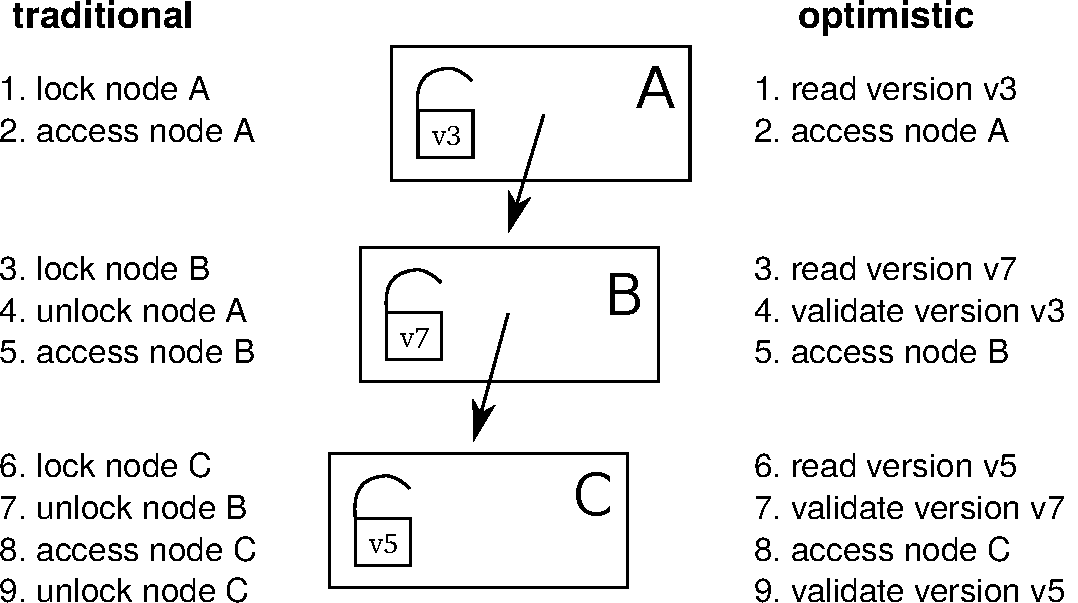
\includegraphics[width=0.65\linewidth]{olcall.pdf}
  \vspace{0.2cm}
  \caption{Comparison of a lookup operation in a 3-level tree using traditional lock coupling (left-hand side) vs.~optimistic lock coupling (right-hand side).}
  \label{fig:olc}
\end{figure}

The traditional and most common lock-based synchronization protocol for B-trees is lock coupling, which interleaves lock acquisitions while holding at most two locks at a time.
If, as we observed earlier, optimistic locks have similar semantics as traditional locks, it is natural to ask whether lock coupling can be combined with optimistic locks.
And indeed the answer is yes: One can almost mechanically translate traditional lock coupling code to optimistic lock coupling code.
This is illustrated in Figure~\ref{fig:olc}, which compares the traversal in a tree of height 3 using traditional and optimistic locks.
As the figure shows, the main difference is that locking is translated to reading the version and that unlocking becomes validation of the previously read version.
This simple change provides efficient lock-free tree traversal without the need to design a complex synchronization protocol.

It is important to emphasize the conceptual simplicity of OLC in comparison to data structures that use custom protocols like the Bw-tree~\cite{DBLP:conf/icde/LevandoskiLS13a}.
To implement lock-free access, the Bw-tree requires an indirection table, delta nodes, complex splitting and merging logic, retry logic, etc.
OLC, on the other hand, can directly be applied to B-trees mostly by adding the appropriate optimistic locking code and without modifying the node layout itself.
Therefore, OpenBw-Tree, an open source implementation of the Bw-tree, requires an order of magnitude more code than a B-tree based on OLC\footnote{Both implementations are available on GitHub: \url{https://github.com/wangziqi2016/index-microbench}}.
Given how difficult it is to develop, validate, and debug lock-free code, simplicity is obviously a major advantage.

\subsection{Correctness Aspects}

\begin{figure}
  % \centering
  %[basicstyle=\normalsize\ttfamily,showstringspaces=false,columns=fullflexible,breaklines=false,breakatwhitespace=true,numbers=none,numberstyle=\small,style=C,keepspaces=true]
\begin{lstlisting}[basicstyle=\ttfamily,language=C++,numbers=left,numberstyle=\small]
std::atomic<BTreeNode*> root;

// search for key in B+tree, returns payload in resultOut
bool lookup(Key key, Value& resultOut) {
   BTreeNode* node = root.load();
   uint64_t nodeVersion = node->readLockOrRestart();
   if (node != root.load()) // make sure the root is still the root
      restart();

   BTreeInner<Key>* parent = nullptr;
   uint64_t parentVersion = 0;

   while (node->isInner()) {
      auto inner = (BTreeInner*)node;

      // unlock parent and make current node the parent
      if (parent)
         parent->readUnlockOrRestart(parentVersion);
      parent = inner;
      parentVersion = nodeVersion;

      // search for next node
      node = inner->findChild(key);
      // validate 'inner' to ensure that 'node' pointer is valid
      inner->checkOrRestart(nodeVersion);
      // now it safe to dereference 'node' pointer (read its version)
      nodeVersion = node->readLockOrRestart();
   }

   // search in leaf and retrieve payload
   auto leaf = (BTreeLeaf*)node;
   bool success = leaf->findValue(key, resultOut);

   // unlock everything
   if (parent)
      parent->readUnlockOrRestart(parentVersion);
   node->readUnlockOrRestart(nodeVersion);

   return success;
}
\end{lstlisting}
  \vspace{0.2cm}
  \caption{B-tree lookup code using OLC. For simplicity, the restart logic is not shown.}
  \label{fig:lookup}
\end{figure}

So far, we have introduced the high-level ideas behind OLC and have stressed its similarity to traditional lock coupling.
Let us now discuss some cases where the close similarity between lock coupling and OLC breaks down.
To make this more concrete, we show the B-tree lookup code in Figure~\ref{fig:lookup}.
In the code, \texttt{readLockOrRestart} reads the lock version and \texttt{readUnlockOrRestart} validates that the read was correct.

One issue with OLC is that any pointer speculatively read from a node may point to invalid memory (if that node is modified concurrently).
Dereferencing such a pointer (e.g., to read its optimistic lock), may cause a segmentation fault or undefined behavior.
In the code shown in Figure~\ref{fig:lookup}, this problem is prevented by the extra check in line 25, which ensures that the read from the node containing the pointer was correct.
Without this additional validation, the code would in line 27 dereference the pointer speculatively read in line 23.
Note that the implementation of \texttt{checkOrRestart} is actually identical to \texttt{readUnlockOrRestart}.
We chose to give it a different name to highlight the fact that this extra check would not be necessary with read/write locks.

Another potential issue with optimistic locks is code that does not terminate.
Code that speculatively accesses a node, like an intra-node binary search, should be written in a way such that it always terminates---even in the presence of concurrent writes.
Otherwise, the validation code that detects the concurrent write will never run.
The binary search of a B-tree, for example, needs to be written in such a way that each comparison makes progress.
For some data structures that do not require loops in the traversal code (like ART) termination is trivially true.

\subsection{Implementation Details}

% implementation, efficiency
To implement an optimistic lock, one can combine the lock and the version counter into a single 64-bit\footnote{Even after subtracting one bit for the lock status, a back-of-the-envelope calculation can show that 63 bits are large enough to never overflow in practice.} word~\cite{artsync}.
A typical read operation will therefore merely consist of reading this version counter atomically.
In C++11 this can be implemented using the \texttt{std::atomic} type.

On x86, atomic reads are cheap because of x86's strong memory order guarantees.
No memory fences are required for sequentially-consistent loads, which are translated (by both GCC and clang) into standard \texttt{MOV} instructions.
Hence, the only effect of \texttt{std::atomic} for loads is preventing instruction re-ordering.
This makes version access and validation cheap.
Acquiring and releasing an optimistic lock in exclusive mode has comparable cost to a traditional lock:
A fairly expensive sequentially-consistent store is needed for acquiring a lock, while a standard \texttt{MOV} suffices for releasing it.
A simple sinlock-based implementation of optimistic locks can be found in the appendix of an earlier paper~\cite{artsync}.

OLC code must be able to handle restarts since validation or lock upgrade can fail due to concurrent writers.
Restarts can easily be implemented by wrapping the data structure operation in a loop (for simplicity not shown in Figure~\ref{fig:lookup}).
Such a loop also enables limiting the number of optimistic retry operations and falling back to pessimistic locking in cases of very heavy contention.
The ability to fall back to traditional locking is a major advantage of OLC in terms of robustness over lock-free approaches, which do not have this option.

In addition to the optimistic shared mode and the exclusive mode, optimistic locks also support a ``shared pessimistic'' mode, which physically acquires the lock in shared mode (allowing multiple concurrent readers but no writers).
This mode is useful for table (or range) scans that touch many tuples on a leaf page (which would otherwise easily abort).
Finally, let us mention that large range scans and table scans, should be broken up into several per-node traversals as is done in the LeanStore~\cite{leanstore} system.

Like all lock-free data structures, but unlike traditional locking and Hardware Transactional Memory~\cite{DBLP:conf/hpca/KarnagelDRLLSL14,DBLP:journals/pvldb/MakreshanskiLS15,htmtkde}, OLC requires care when deleting (and reusing) nodes.
The reason is that a deleting thread can never be sure that a node can be reclaimed because other threads might still be optimistically reading from that node.
Therefore, standard solutions like epoch-based reclamation~\cite{DBLP:conf/sosp/TuZKLM13}, hazard pointers~\cite{DBLP:journals/tpds/Michael04}, or optimized hazard pointers~\cite{DBLP:conf/spaa/BalmauGHZ16} need to be used.
These memory reclamation techniques are, however, largely orthogonal to the synchronization protocol itself.

%-lock-free is not a strong guarantee

\newpage
\section{Evaluation}\label{sec:evaluation}

Let us now experimentally evaluate the overhead and scalability of OLC.
For the experiments, we use an in-memory B+tree implemented in C++11 using templates, which is configured to use nodes of 4096 bytes, random 8 byte keys, and 8 byte payloads.
Based on this B-tree, we compare the following synchronization approaches:
\begin{itemize}
\item an OLC implementation\footnote{An almost identical OLC implementation is available on github: \url{https://github.com/wangziqi2016/index-microbench/tree/master/BTreeOLC}}
\item a variant based on traditional lock coupling and read/write locks
\item the unsynchronized B-tree, which obviously is only correct for read-only workloads but allows measuring the overhead of synchronization
\end{itemize}
Note that earlier work has compared the OLC implementation with a Bw-tree implementation~\cite{buzzword} and other state-of-the-art in-memory index structures.

We use a Haswell EP system with an Intel Xeon E5-2687W v3 CPU, which has 10 cores (20 ``Hyper-Threads'') and 25~MB of L3 cache.
The system is running Ubuntu 18.10 and we use GCC 8.2.0 to compile our code.
The CPU counters are obtained using the Linux perf API\footnote{We use the following convenience wrapper: \url{https://github.com/viktorleis/perfevent}}.

\begin{table}
  \caption{Performance and CPU counters for lookup and insert operations in a B-tree with 100M keys. We perform 100M operations and normalize the CPU counters by that number.}
  \label{tab:overhead}
  \centering
  \begin{tabular}{lrrrrrrr}\toprule
                    &         &        &        & instruc-  & L1     & L3     & branch \\
                    & threads & M op/s & cycles & tions & misses & misses & misses \\\midrule
lookup (no sync.)   & 1       & 1.72   & 2028   & 283     & 39.1   & 14.9   & 16.1   \\
lookup (OLC)        & 1       & 1.65   & 2107   & 370     & 43.9   & 15.1   & 16.7   \\
lookup (lock coup.) & 1       & 1.72   & 2078   & 365     & 42.3   & 16.9   & 15.7   \\\midrule
insert (no sync.)   & 1       & 1.51   & 2286   & 530     & 59.8   & 31.1   & 17.3   \\
insert (OLC)        & 1       & 1.50   & 2303   & 629     & 61.2   & 31.1   & 16.5   \\
insert (lock coup.) & 1       & 1.41   & 2473   & 644     & 61.0   & 31.0   & 17.2   \\\midrule
lookup (no sync.)   & 10      & 15.48  & 2058   & 283     & 38.6   & 15.5   & 16.0   \\
lookup (OLC)        & 10      & 14.60  & 2187   & 370     & 43.8   & 15.8   & 16.8   \\
lookup (lock coup.) & 10      & 5.71   & 5591   & 379     & 54.2   & 17.0   & 14.8   \\\midrule
insert (no sync.)   & 10      & -      & -      & -       & -      & -      & -      \\
insert (OLC)        & 10      & 10.46  & 2940   & 656     & 62.0   & 32.5   & 16.8   \\
insert (lock coup.) & 10      & 7.55   & 4161   & 667     & 75.0   & 28.6   & 16.2   \\
    \bottomrule
\end{tabular}
\end{table}

Table~\ref{tab:overhead} compares the performance and CPU counters for lookup and insert operations in a B-tree with 100M keys.
With {\em single-threaded} execution, we observe that all three approaches have very similar performance.
Adding traditional or optimistic locks to unsynchronized B-tree code results in up to 30\% of additional instructions without affecting single-threaded performance much.

\begin{figure}
  \centering
  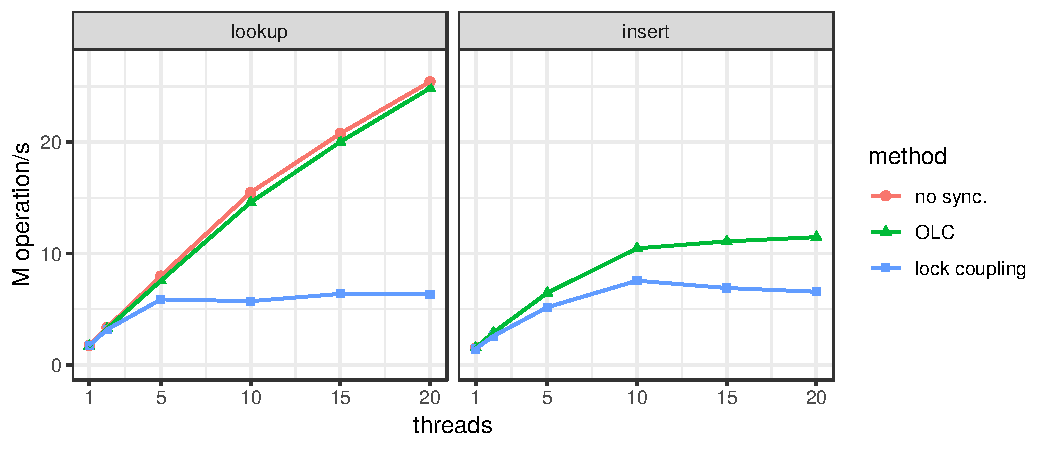
\includegraphics[width=\linewidth]{scale.pdf}
  \vspace{0.2cm}
  \caption{Scalability on 10-core system for B-tree operations (100M values).}
  \label{fig:scale}
\end{figure}

As Figure~\ref{fig:scale} shows, the results change dramatically once we use multiple threads.
For lookup, the scalability of OLC is near-linear up to 20 threads, even though the system has only 10 ``real cores''.
The OLC scalability for insert is also respectable (though not quite as linear because multi-threaded insertion approaches the memory bandwidth of our processor).
The figure also shows that the results of traditional lock coupling with read/write locks are significantly worse than OLC.
With 20 threads, lookup with OLC is 3.9$\times$ faster than traditional lock coupling.

\section{Summary}\label{sec:conc}

Optimistic Lock Coupling (OLC) is an effective synchronization method that combines the simplicity of traditional lock coupling with the superior scalability of lock-free approaches.
OLC is widely applicable and has already been successfully used to synchronize several data structures, including B-trees, binary search trees, and different trie variants.
These features make it highly attractive for modern database systems as well as performance-critical systems software in general.

\begin{thebibliography}{10}

\bibitem{DBLP:conf/spaa/BalmauGHZ16}
O.~Balmau, R.~Guerraoui, M.~Herlihy, and I.~Zablotchi.
\newblock Fast and robust memory reclamation for concurrent data structures.
\newblock In {\em SPAA}, 2016.

\bibitem{DBLP:journals/acta/BayerS77}
R.~Bayer and M.~Schkolnick.
\newblock Concurrency of operations on {B}-trees.
\newblock {\em Acta Informatica}, 9, 1977.

\bibitem{hot}
R.~Binna, E.~Zangerle, M.~Pichl, G.~Specht, and V.~Leis.
\newblock {HOT}: A height optimized trie index for main-memory database
  systems.
\newblock In {\em SIGMOD}, 2018.

\bibitem{DBLP:conf/ppopp/BronsonCCO10}
N.~G. Bronson, J.~Casper, H.~Chafi, and K.~Olukotun.
\newblock A practical concurrent binary search tree.
\newblock In {\em PPOPP}, 2010.

\bibitem{DBLP:conf/vldb/ChaHKK01}
S.~K. Cha, S.~Hwang, K.~Kim, and K.~Kwon.
\newblock Cache-conscious concurrency control of main-memory indexes on
  shared-memory multiprocessor systems.
\newblock In {\em VLDB}, 2001.

\bibitem{intel}
I.~Cutress.
\newblock {Intel} goes for 48-cores: {Cascade-AP} with multi-chip package
  coming soon.
\newblock
  \url{https://www.anandtech.com/show/13535/intel-goes-for-48cores-cascade-ap},
  2018 (accessed January, 2019).

\bibitem{DBLP:conf/cidr/FaleiroA17}
J.~M. Faleiro and D.~J. Abadi.
\newblock Latch-free synchronization in database systems: Silver bullet or
  fool's gold?
\newblock In {\em CIDR}, 2017.

\bibitem{DBLP:journals/ftdb/Graefe11}
G.~Graefe.
\newblock Modern {B}-tree techniques.
\newblock {\em Foundations and Trends in Databases}, 3(4), 2011.

\bibitem{DBLP:conf/hpca/KarnagelDRLLSL14}
T.~Karnagel, R.~Dementiev, R.~Rajwar, K.~Lai, T.~Legler, B.~Schlegel, and
  W.~Lehner.
\newblock Improving in-memory database index performance with
  {Intel}\({}^{\mbox{{\textregistered}}}\) transactional synchronization
  extensions.
\newblock In {\em HPCA}, 2014.

\bibitem{DBLP:journals/tods/LehmanY81}
P.~L. Lehman and S.~B. Yao.
\newblock Efficient locking for concurrent operations on {B}-trees.
\newblock {\em {ACM} Trans. Database Syst.}, 6(4), 1981.

\bibitem{leanstore}
V.~Leis, M.~Haubenschild, A.~Kemper, and T.~Neumann.
\newblock Leanstore: In-memory data management beyond main memory.
\newblock In {\em ICDE}, 2018.

\bibitem{art}
V.~Leis, A.~Kemper, and T.~Neumann.
\newblock The adaptive radix tree: {ARTful} indexing for main-memory databases.
\newblock In {\em ICDE}, 2013.

\bibitem{htmtkde}
V.~Leis, A.~Kemper, and T.~Neumann.
\newblock Scaling {HTM}-supported database transactions to many cores.
\newblock {\em {IEEE} Trans. Knowl. Data Eng.}, 28(2), 2016.

\bibitem{artsync}
V.~Leis, F.~Scheibner, A.~Kemper, and T.~Neumann.
\newblock The {ART} of practical synchronization.
\newblock In {\em DaMoN}, 2016.

\bibitem{DBLP:conf/icde/LevandoskiLS13a}
J.~J. Levandoski, D.~B. Lomet, and S.~Sengupta.
\newblock The {Bw}-tree: A {B}-tree for new hardware platforms.
\newblock In {\em ICDE}, 2013.

\bibitem{DBLP:journals/pvldb/MakreshanskiLS15}
D.~Makreshanski, J.~J. Levandoski, and R.~Stutsman.
\newblock To lock, swap, or elide: On the interplay of hardware transactional
  memory and lock-free indexing.
\newblock {\em {PVLDB}}, 8(11), 2015.

\bibitem{DBLP:dblp_conf/eurosys/MaoKM12}
Y.~Mao, E.~Kohler, and R.~T. Morris.
\newblock Cache craftiness for fast multicore key-value storage.
\newblock In {\em EuroSys}, 2012.

\bibitem{DBLP:journals/tpds/Michael04}
M.~M. Michael.
\newblock Hazard pointers: Safe memory reclamation for lock-free objects.
\newblock {\em {IEEE} Trans. Parallel Distrib. Syst.}, 15(6), 2004.

\bibitem{DBLP:journals/jacm/ShalevS06}
O.~Shalev and N.~Shavit.
\newblock Split-ordered lists: Lock-free extensible hash tables.
\newblock {\em J. {ACM}}, 53(3), 2006.

\bibitem{amd}
A.~Shilov.
\newblock {AMD} previews {EPYC} ‘{Rome}’ processor: Up to 64 {Zen} 2 cores.
\newblock
  \url{https://www.anandtech.com/show/13561/amd-previews-epyc-rome-processor-up-to-64-zen-2-cores},
  2018 (accessed January, 2019).

\bibitem{DBLP:conf/sosp/TuZKLM13}
S.~Tu, W.~Zheng, E.~Kohler, B.~Liskov, and S.~Madden.
\newblock Speedy transactions in multicore in-memory databases.
\newblock In {\em SOSP}, 2013.

\bibitem{buzzword}
Z.~Wang, A.~Pavlo, H.~Lim, V.~Leis, H.~Zhang, M.~Kaminsky, and D.~Andersen.
\newblock Building a {Bw}-tree takes more than just buzz words.
\newblock In {\em SIGMOD}, 2018.

\end{thebibliography}


%\bibliographystyle{abbrv}
%\bibliography{main}

\end{document}

\end{article}


\begin{article}
{Report from the Workshop on Common Model Infrastructure, {ACM KDD 2018}}
{Chaitanya Baru}
\pdfminorversion=5
\documentclass[11pt]{article}
\usepackage{deauthor,times,graphicx,caption,microtype}
\usepackage{hyperref}
\usepackage{listings}
\usepackage{booktabs}

\begin{document}

\title{Optimistic Lock Coupling: A Scalable and Efficient General-Purpose Synchronization Method}

\author{Viktor Leis, Michael Haubenschild\raisebox{0.9ex}{$\ast$}, Thomas Neumann\\ Technische Universit{\"a}t M{\"u}nchen \hspace{0.7cm} Tableau Software\raisebox{0.9ex}{$\ast$} \\ {\{leis,neumann\}{@}in.tum.de} \hspace{0.7cm} {mhaubenschild{@}tableau.com\raisebox{0.9ex}{$\ast$}}}

\maketitle

\begin{abstract}
As the number of cores on commodity processors continues to increase, scalability becomes more and more crucial for overall performance.
Scalable and efficient concurrent data structures are particularly important, as these are often the building blocks of parallel algorithms.
Unfortunately, traditional synchronization techniques based on fine-grained locking have been shown to be unscalable on modern multi-core CPUs.
Lock-free data structures, on the other hand, are extremely difficult to design and often incur significant overhead.

In this work, we make the case for Optimistic Lock Coupling as a practical alternative to both traditional locking and the lock-free approach.
We show that Optimistic Lock Coupling is highly scalable and almost as simple to implement as traditional lock coupling.
Another important advantage is that it is easily applicable to most tree-like data structures.
We therefore argue that Optimistic Lock Coupling, rather than a complex and error-prone custom synchronization protocol, should be the default choice for performance-critical data structures.
\end{abstract}

\section{Introduction}

% more and more cores
Today, Intel's commodity server processors have up to 28 cores and its upcoming microarchitecture will have up to 48 cores per socket~\cite{intel}.
Similarly, AMD currently stands at 32 cores and this number is expected to double in the next generation~\cite{amd}.
Since both platforms support simultaneous multithreading (also known as hyperthreading), affordable commodity servers (with up to two sockets) will soon routinely have between 100 and 200 hardware threads.

% data structure scalability is important
With such a high degree of hardware parallelism, efficient data processing crucially depends on how well concurrent data structures scale.
Internally, database systems use a plethora of data structures like table heaps, internal work queues, and, most importantly, index structures.
Any of these can easily become a scalability (and therefore overall performance) bottleneck on many-core CPUs.

% traditional synchronization: fine-grained locks, slow, cache invalidation
Traditionally, database systems synchronize internal data structures using fine-grained reader/writer locks\footnote{In this work, we focus on data structure synchronization rather than high-level transaction semantics and therefore use the term {\em lock} for what would typically be called {\em latch} in the database literature. We thus follow common computer science (rather than database) terminology.}.
Unfortunately, while fine-grained locking makes lock contention unlikely, it still results in bad scalability because lock acquisition and release require writing to shared memory.
Due to the way cache coherency is implemented on modern multi-core CPUs, these writes cause additional cache misses\footnote{The cache coherency protocol ensures that all copies of a cache line on other cores are invalidated before the write can proceed.} and the cache line containing the lock's internal data becomes a point of physical contention.
As a result, any frequently-accessed lock (e.g., the lock of the root node of a B-tree) severely limits scalability.

% lock-free bw-tree: no more latches, but indirections, extremely complex
Lock-free data structures like the Bw-tree~\cite{DBLP:conf/icde/LevandoskiLS13a} (a lock-free B-tree variant) or the Split-Ordered List~\cite{DBLP:journals/jacm/ShalevS06} (a lock-free hash table) do not acquire any locks and therefore generally scale much better than locking-based approaches (in particular for read-mostly workloads).
However, lock-free synchronization has other downsides:
First, it is very difficult and results in extremely complex and error-prone code (when compared to locking).
Second, because the functionality of atomic primitives provided by the hardware (e.g., atomically compare-and-swap 8 bytes) is limited, complex operations require additional indirections within the data structure.
For example, the Bw-tree requires an indirection table and the Split-Ordered List requires ``dummy nodes'', resulting in overhead due to additional cache misses.

% OLC for the win
In this paper we make the case for {\em Optimistic Lock Coupling (OLC)}, a synchronization method that combines some of the best properties of lock-based and lock-free synchronization.
OLC utilizes a special lock type that can be used in two modes:
The first mode is similar to a traditional mutex and excludes other threads by physically acquiring the underlying lock.
In the second mode, reads can proceed optimistically by validating a version counter that is embedded in the lock (similar to optimistic concurrency control).
The first mode is typically used by writers and the second mode by readers.
Besides this special lock type, OLC is based on the observation that optimistic lock validations can be interleaved/coupled---similar to the pair-wise interleaved lock acquisition of traditional lock coupling.
Hence, the name Optimistic Lock Coupling.

OLC has a number of desirable features:
\begin{itemize}
\item By reducing the number of writes to shared memory locations and thereby avoiding cache invalidations, it {\bf scales well} for most workloads.
\item In comparison to unsynchronized code, it requires few additional CPU instructions making it {\bf efficient}.
\item OLC is {\bf widely applicable} to different data structures. It has already been successfully used for synchronizing binary search trees~\cite{DBLP:conf/ppopp/BronsonCCO10}, tries~\cite{artsync}, trie/B-tree hybrids~\cite{DBLP:dblp_conf/eurosys/MaoKM12}, and B-trees~\cite{buzzword}.
\item In comparison to the lock-free paradigm, it is also {\bf easy to use} and requires few modifications to existing, single-threaded data structures.
\end{itemize}
Despite these positive features and its simplicity, OLC is not yet widely known.
The goal of this paper is therefore to popularize this simple idea and to make a case for it.
We argue that OLC deserves to be widely known.
It is a good default synchronization paradigm---more complex, data structure-specific protocols are seldom beneficial.

The rest of the paper is organized as follows.
Section~\ref{sec:related} discusses related work, tracing the history of OLC and its underlying ideas in the literature.
The core of the paper is Section~\ref{sec:olc}, which describes the ideas behind OLC and how it can be used to synchronize complex data structures.
In Section~\ref{sec:evaluation} we experimentally show that OLC has low overhead and scales well when used to synchronize an in-memory B-tree.
We summarize the paper in Section~\ref{sec:conc}.

\newpage
\section{Related Work}\label{sec:related}

Lock coupling has been proposed as a method for allowing concurrent operations on B-trees in 1977~\cite{DBLP:journals/acta/BayerS77}.
This traditional and still widely-used method, described in detail in Graefe's B-tree survey~\cite{DBLP:journals/ftdb/Graefe11}, is also called ``latch coupling'', ``hand-over-hand locking'', and ``crabbing''.
Because at most two locks are held at-a-time during tree traversal, this technique seemingly allows for a high degree of parallelism---in particular if read/write locks are used to enable inner nodes to be locked in shared mode.
However, as we show in Section~\ref{sec:evaluation}, on modern hardware lock acquisition (even in shared mode) results in suboptimal scalability.

An early alternative from 1981 is a B-tree variant called B-link tree~\cite{DBLP:journals/tods/LehmanY81}, which only holds a single lock at a time.
It is based on the observation that between the release of the parent lock and the acquisition of the child lock, the only ``dangerous'' thing that could have happened is the split of a child node (assuming one does not implement merge operations).
Thus, when a split happens, the key being searched might end up on a neighboring node to the right of the current child node.
A B-link tree traversal therefore detects this condition and, if needed, transparently proceeds to the neighboring node.
Releasing the parent lock early is highly beneficial when the child node needs to be fetched from disk.
For in-memory workloads, however, the B-link tree has the same scalability issues as lock coupling (it acquires just as many locks).

The next major advance, Optimistic Latch-Free Index Traversal (OLFIT)~\cite{DBLP:conf/vldb/ChaHKK01}, was proposed in 2001.
OLFIT introduced the idea of a combined lock/update counter, which we call {\em optimistic lock}. % , for lack of a better name,
Based on these per-node optimistic locks and the synchronization protocol of the B-link tree, OLFIT finally achieves good scalability on parallel processors.
The OLFIT protocol is fairly complex, as it requires both the non-trivial B-link protocol and optimistic locks.
Furthermore, like the B-link tree protocol, it does not support merging nodes, and is specific to B-trees (cannot easily be applied to other data structures).

In the following two decades, the growth of main-memory capacity led to much research into other data structures besides the venerable B-tree.
Particularly relevant for our discussion is Bronson et al.'s~\cite{DBLP:conf/ppopp/BronsonCCO10} concurrent binary search tree, which is based on optimistic version validation and has a sophisticated, data structure-specific synchronization protocol.
To the best of our knowledge, this 2010 paper is the first that, as part of its protocol, interleaves version validation across nodes---rather than validating each node separately like OLFIT.
In that paper, this idea is called ``hand-over-hand, optimistic validation'', while we prefer the term Optimistic Lock Coupling to highlight the close resemblance to traditional lock coupling.
Similarly, Mao et al.'s~\cite{DBLP:dblp_conf/eurosys/MaoKM12} Masstree (a concurrent hybrid trie/B-tree) is also based on the same ideas, but again uses them as part of a more complex protocol.

The Adaptive Radix Tree (ART)~\cite{art} is another recent in-memory data structure, which we proposed in 2013.
In contrast to the two data structures just mentioned, it was originally designed with single-threaded performance in mind without supporting concurrency.
To add support for concurrency, we initially started designing a custom protocol called Read-Optimized Write Exclusion (ROWEX)~\cite{artsync}, which turned out to be non-trivial and requires modifications of the underlying data structure\footnote{Note that ROWEX is already easier to apply to existing data structures than the lock-free approach. The difficulty depends on the data structure. Applying ROWEX is hard for B-trees with sorted keys and fairly easy for copy-on-write data structures like the Height Optimized Trie~\cite{hot}---with ART being somewhere in the middle.}.
However, fairly late in the project, we also realized, that OLC {\em alone} (rather than as part of a more complex protocol) is sufficient to synchronize ART.
No other changes to the data structure were necessary.
Both approaches were published and experimentally evaluated in a followup paper~\cite{artsync}, which shows that, despite its simplicity, OLC is efficient, scalable, and generally outperforms ROWEX.

Similar results were recently published regarding B-trees~\cite{buzzword}.
In this experimental study a simple OLC-based synchronization outperformed the Bw-tree~\cite{DBLP:conf/icde/LevandoskiLS13a}, a complex lock-free synchronization approach.
Another recent paper shows that for write-intensive workloads, locking often performs better than lock-free synchronization~\cite{DBLP:conf/cidr/FaleiroA17}.
These experiences indicate that OLC is a general-purpose synchronization paradigm and motivate the current paper.

%foster b-tree\cite{DBLP:journals/tods/GraefeKK12}
%Shasha theory~\cite{DBLP:journals/tods/ShashaG88}

\section{Optimistic Lock Coupling}\label{sec:olc}

% locks suck
The standard technique for inter-thread synchronization is mutual exclusion using fine-grained locks.
In a B-tree, for example, every node usually has its own associated lock, which is acquired before accessing that node.
The problem of locking on modern multi- and many-core processors is that lock acquisition and release require writing to the shared memory location that implements the lock.
This write causes exclusive ownership of the underlying cache line and invalidates copies of it on all other processor cores.
For hierarchical, tree-like data structures, the lock of the root node becomes a point of physical contention---even in read-only workloads and even when read/write locks are used.
Depending on the specific data structure, number of cores, cache coherency protocol implementation, cache topology, whether Non-Uniform Memory Access (NUMA) is used, locking can even result in multi-threaded performance that is worse than single-threaded execution.

% in b-trees this happens very much
The inherent pessimism of locking is particularly unfortunate for B-trees:
Despite the fact that logical modifications of the root node are very infrequent, every B-tree operation must lock the root node during tree traversal\footnote{To a lesser extent this obviously applies to all inner nodes, not just the root.}.
Even the vast majority of update operations (with the exception of splits and merges), only modify a single leaf node.
These observations indicate that a more optimistic approach, which does not require locking inner nodes, would be very beneficial for B-trees.

\subsection{Optimistic Locks}

% optimism to the rescue
As the name indicates, optimistic locks try to solve the scalability issues of traditional locks using an optimistic approach.
Instead of always physically acquiring locks, even for nodes that are unlikely to be modified simultaneously, after-the-fact validation is used to detect conflicts.
This is done by augmenting each lock with a version/update counter that is incremented on every modification.
Using this version counter, readers can optimistically proceed before validating that the version did not change to ensure that the read was safe.
If validation fails, the operation is restarted.

% details on opt locks
Using optimistic locks, a read-only node access (i.e., the majority of all operations in a B-tree) does not acquire the lock and does not increment the version counter.
Instead, it performs the following steps:
\begin{enumerate}
\item read lock version (restart if lock is not free)
\item access node
\item read the version again and validate that it has not changed in the meantime
\end{enumerate}
If the last step (the validation) fails, the operation has to be restarted.
Write operations, on the other hand, are more similar to traditional locking:
\begin{enumerate}
\item acquire lock (wait if necessary)
\item access/write to node
\item increment version and unlock node
\end{enumerate}
Writes can therefore protect a node from other writes.

% similar to locks
As we observed in an earlier paper~\cite{artsync}, because of similar semantics, optimistic locks can be hidden behind an API very similar to traditional read/write locks.
Both approaches have an exclusive lock mode, and acquiring a traditional lock in shared mode is analogous to optimistic version validation.
Furthermore, like with some implementations of traditional read/write locks, optimistic locks allow upgrading a shared lock to an exclusive lock.
Lock upgrades are, for example, used to avoid most B-tree update operations from having to lock inner nodes.
In our experience, the close resemblance of optimistic and traditional locks simplifies the reasoning about optimistic locks;
one can apply similar thinking as in traditional lock-based protocols.

\subsection{Lock Coupling with Optimistic Locks}

\begin{figure}
  \centering
  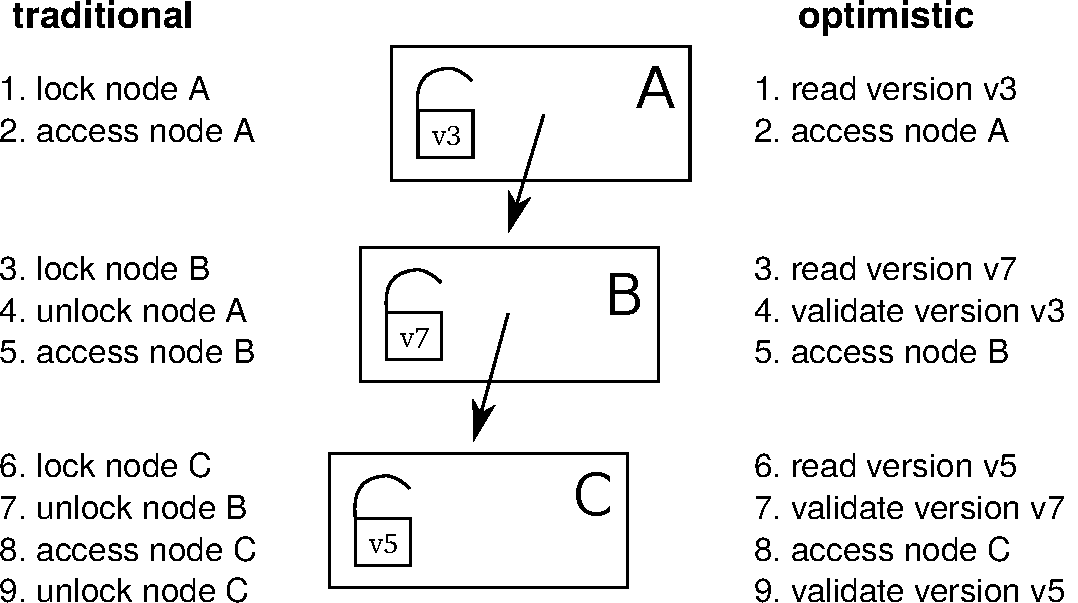
\includegraphics[width=0.65\linewidth]{olcall.pdf}
  \vspace{0.2cm}
  \caption{Comparison of a lookup operation in a 3-level tree using traditional lock coupling (left-hand side) vs.~optimistic lock coupling (right-hand side).}
  \label{fig:olc}
\end{figure}

The traditional and most common lock-based synchronization protocol for B-trees is lock coupling, which interleaves lock acquisitions while holding at most two locks at a time.
If, as we observed earlier, optimistic locks have similar semantics as traditional locks, it is natural to ask whether lock coupling can be combined with optimistic locks.
And indeed the answer is yes: One can almost mechanically translate traditional lock coupling code to optimistic lock coupling code.
This is illustrated in Figure~\ref{fig:olc}, which compares the traversal in a tree of height 3 using traditional and optimistic locks.
As the figure shows, the main difference is that locking is translated to reading the version and that unlocking becomes validation of the previously read version.
This simple change provides efficient lock-free tree traversal without the need to design a complex synchronization protocol.

It is important to emphasize the conceptual simplicity of OLC in comparison to data structures that use custom protocols like the Bw-tree~\cite{DBLP:conf/icde/LevandoskiLS13a}.
To implement lock-free access, the Bw-tree requires an indirection table, delta nodes, complex splitting and merging logic, retry logic, etc.
OLC, on the other hand, can directly be applied to B-trees mostly by adding the appropriate optimistic locking code and without modifying the node layout itself.
Therefore, OpenBw-Tree, an open source implementation of the Bw-tree, requires an order of magnitude more code than a B-tree based on OLC\footnote{Both implementations are available on GitHub: \url{https://github.com/wangziqi2016/index-microbench}}.
Given how difficult it is to develop, validate, and debug lock-free code, simplicity is obviously a major advantage.

\subsection{Correctness Aspects}

\begin{figure}
  % \centering
  %[basicstyle=\normalsize\ttfamily,showstringspaces=false,columns=fullflexible,breaklines=false,breakatwhitespace=true,numbers=none,numberstyle=\small,style=C,keepspaces=true]
\begin{lstlisting}[basicstyle=\ttfamily,language=C++,numbers=left,numberstyle=\small]
std::atomic<BTreeNode*> root;

// search for key in B+tree, returns payload in resultOut
bool lookup(Key key, Value& resultOut) {
   BTreeNode* node = root.load();
   uint64_t nodeVersion = node->readLockOrRestart();
   if (node != root.load()) // make sure the root is still the root
      restart();

   BTreeInner<Key>* parent = nullptr;
   uint64_t parentVersion = 0;

   while (node->isInner()) {
      auto inner = (BTreeInner*)node;

      // unlock parent and make current node the parent
      if (parent)
         parent->readUnlockOrRestart(parentVersion);
      parent = inner;
      parentVersion = nodeVersion;

      // search for next node
      node = inner->findChild(key);
      // validate 'inner' to ensure that 'node' pointer is valid
      inner->checkOrRestart(nodeVersion);
      // now it safe to dereference 'node' pointer (read its version)
      nodeVersion = node->readLockOrRestart();
   }

   // search in leaf and retrieve payload
   auto leaf = (BTreeLeaf*)node;
   bool success = leaf->findValue(key, resultOut);

   // unlock everything
   if (parent)
      parent->readUnlockOrRestart(parentVersion);
   node->readUnlockOrRestart(nodeVersion);

   return success;
}
\end{lstlisting}
  \vspace{0.2cm}
  \caption{B-tree lookup code using OLC. For simplicity, the restart logic is not shown.}
  \label{fig:lookup}
\end{figure}

So far, we have introduced the high-level ideas behind OLC and have stressed its similarity to traditional lock coupling.
Let us now discuss some cases where the close similarity between lock coupling and OLC breaks down.
To make this more concrete, we show the B-tree lookup code in Figure~\ref{fig:lookup}.
In the code, \texttt{readLockOrRestart} reads the lock version and \texttt{readUnlockOrRestart} validates that the read was correct.

One issue with OLC is that any pointer speculatively read from a node may point to invalid memory (if that node is modified concurrently).
Dereferencing such a pointer (e.g., to read its optimistic lock), may cause a segmentation fault or undefined behavior.
In the code shown in Figure~\ref{fig:lookup}, this problem is prevented by the extra check in line 25, which ensures that the read from the node containing the pointer was correct.
Without this additional validation, the code would in line 27 dereference the pointer speculatively read in line 23.
Note that the implementation of \texttt{checkOrRestart} is actually identical to \texttt{readUnlockOrRestart}.
We chose to give it a different name to highlight the fact that this extra check would not be necessary with read/write locks.

Another potential issue with optimistic locks is code that does not terminate.
Code that speculatively accesses a node, like an intra-node binary search, should be written in a way such that it always terminates---even in the presence of concurrent writes.
Otherwise, the validation code that detects the concurrent write will never run.
The binary search of a B-tree, for example, needs to be written in such a way that each comparison makes progress.
For some data structures that do not require loops in the traversal code (like ART) termination is trivially true.

\subsection{Implementation Details}

% implementation, efficiency
To implement an optimistic lock, one can combine the lock and the version counter into a single 64-bit\footnote{Even after subtracting one bit for the lock status, a back-of-the-envelope calculation can show that 63 bits are large enough to never overflow in practice.} word~\cite{artsync}.
A typical read operation will therefore merely consist of reading this version counter atomically.
In C++11 this can be implemented using the \texttt{std::atomic} type.

On x86, atomic reads are cheap because of x86's strong memory order guarantees.
No memory fences are required for sequentially-consistent loads, which are translated (by both GCC and clang) into standard \texttt{MOV} instructions.
Hence, the only effect of \texttt{std::atomic} for loads is preventing instruction re-ordering.
This makes version access and validation cheap.
Acquiring and releasing an optimistic lock in exclusive mode has comparable cost to a traditional lock:
A fairly expensive sequentially-consistent store is needed for acquiring a lock, while a standard \texttt{MOV} suffices for releasing it.
A simple sinlock-based implementation of optimistic locks can be found in the appendix of an earlier paper~\cite{artsync}.

OLC code must be able to handle restarts since validation or lock upgrade can fail due to concurrent writers.
Restarts can easily be implemented by wrapping the data structure operation in a loop (for simplicity not shown in Figure~\ref{fig:lookup}).
Such a loop also enables limiting the number of optimistic retry operations and falling back to pessimistic locking in cases of very heavy contention.
The ability to fall back to traditional locking is a major advantage of OLC in terms of robustness over lock-free approaches, which do not have this option.

In addition to the optimistic shared mode and the exclusive mode, optimistic locks also support a ``shared pessimistic'' mode, which physically acquires the lock in shared mode (allowing multiple concurrent readers but no writers).
This mode is useful for table (or range) scans that touch many tuples on a leaf page (which would otherwise easily abort).
Finally, let us mention that large range scans and table scans, should be broken up into several per-node traversals as is done in the LeanStore~\cite{leanstore} system.

Like all lock-free data structures, but unlike traditional locking and Hardware Transactional Memory~\cite{DBLP:conf/hpca/KarnagelDRLLSL14,DBLP:journals/pvldb/MakreshanskiLS15,htmtkde}, OLC requires care when deleting (and reusing) nodes.
The reason is that a deleting thread can never be sure that a node can be reclaimed because other threads might still be optimistically reading from that node.
Therefore, standard solutions like epoch-based reclamation~\cite{DBLP:conf/sosp/TuZKLM13}, hazard pointers~\cite{DBLP:journals/tpds/Michael04}, or optimized hazard pointers~\cite{DBLP:conf/spaa/BalmauGHZ16} need to be used.
These memory reclamation techniques are, however, largely orthogonal to the synchronization protocol itself.

%-lock-free is not a strong guarantee

\newpage
\section{Evaluation}\label{sec:evaluation}

Let us now experimentally evaluate the overhead and scalability of OLC.
For the experiments, we use an in-memory B+tree implemented in C++11 using templates, which is configured to use nodes of 4096 bytes, random 8 byte keys, and 8 byte payloads.
Based on this B-tree, we compare the following synchronization approaches:
\begin{itemize}
\item an OLC implementation\footnote{An almost identical OLC implementation is available on github: \url{https://github.com/wangziqi2016/index-microbench/tree/master/BTreeOLC}}
\item a variant based on traditional lock coupling and read/write locks
\item the unsynchronized B-tree, which obviously is only correct for read-only workloads but allows measuring the overhead of synchronization
\end{itemize}
Note that earlier work has compared the OLC implementation with a Bw-tree implementation~\cite{buzzword} and other state-of-the-art in-memory index structures.

We use a Haswell EP system with an Intel Xeon E5-2687W v3 CPU, which has 10 cores (20 ``Hyper-Threads'') and 25~MB of L3 cache.
The system is running Ubuntu 18.10 and we use GCC 8.2.0 to compile our code.
The CPU counters are obtained using the Linux perf API\footnote{We use the following convenience wrapper: \url{https://github.com/viktorleis/perfevent}}.

\begin{table}
  \caption{Performance and CPU counters for lookup and insert operations in a B-tree with 100M keys. We perform 100M operations and normalize the CPU counters by that number.}
  \label{tab:overhead}
  \centering
  \begin{tabular}{lrrrrrrr}\toprule
                    &         &        &        & instruc-  & L1     & L3     & branch \\
                    & threads & M op/s & cycles & tions & misses & misses & misses \\\midrule
lookup (no sync.)   & 1       & 1.72   & 2028   & 283     & 39.1   & 14.9   & 16.1   \\
lookup (OLC)        & 1       & 1.65   & 2107   & 370     & 43.9   & 15.1   & 16.7   \\
lookup (lock coup.) & 1       & 1.72   & 2078   & 365     & 42.3   & 16.9   & 15.7   \\\midrule
insert (no sync.)   & 1       & 1.51   & 2286   & 530     & 59.8   & 31.1   & 17.3   \\
insert (OLC)        & 1       & 1.50   & 2303   & 629     & 61.2   & 31.1   & 16.5   \\
insert (lock coup.) & 1       & 1.41   & 2473   & 644     & 61.0   & 31.0   & 17.2   \\\midrule
lookup (no sync.)   & 10      & 15.48  & 2058   & 283     & 38.6   & 15.5   & 16.0   \\
lookup (OLC)        & 10      & 14.60  & 2187   & 370     & 43.8   & 15.8   & 16.8   \\
lookup (lock coup.) & 10      & 5.71   & 5591   & 379     & 54.2   & 17.0   & 14.8   \\\midrule
insert (no sync.)   & 10      & -      & -      & -       & -      & -      & -      \\
insert (OLC)        & 10      & 10.46  & 2940   & 656     & 62.0   & 32.5   & 16.8   \\
insert (lock coup.) & 10      & 7.55   & 4161   & 667     & 75.0   & 28.6   & 16.2   \\
    \bottomrule
\end{tabular}
\end{table}

Table~\ref{tab:overhead} compares the performance and CPU counters for lookup and insert operations in a B-tree with 100M keys.
With {\em single-threaded} execution, we observe that all three approaches have very similar performance.
Adding traditional or optimistic locks to unsynchronized B-tree code results in up to 30\% of additional instructions without affecting single-threaded performance much.

\begin{figure}
  \centering
  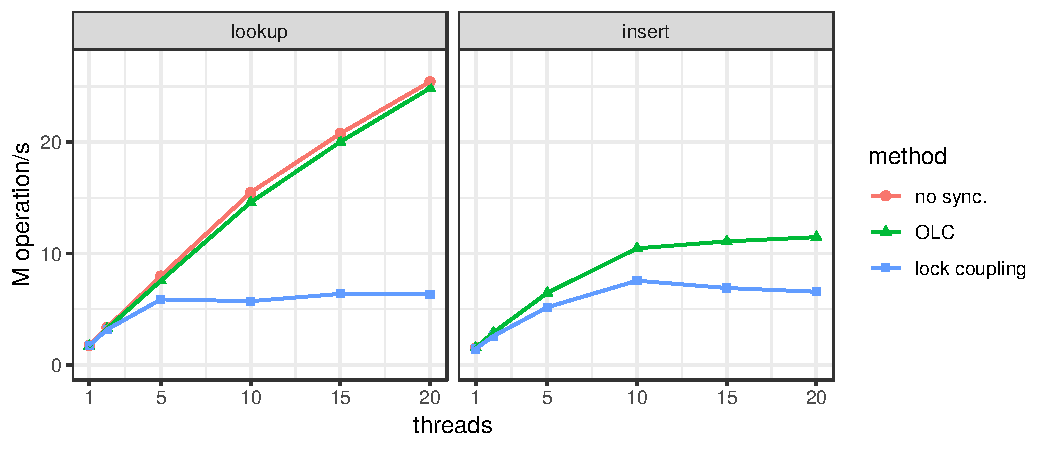
\includegraphics[width=\linewidth]{scale.pdf}
  \vspace{0.2cm}
  \caption{Scalability on 10-core system for B-tree operations (100M values).}
  \label{fig:scale}
\end{figure}

As Figure~\ref{fig:scale} shows, the results change dramatically once we use multiple threads.
For lookup, the scalability of OLC is near-linear up to 20 threads, even though the system has only 10 ``real cores''.
The OLC scalability for insert is also respectable (though not quite as linear because multi-threaded insertion approaches the memory bandwidth of our processor).
The figure also shows that the results of traditional lock coupling with read/write locks are significantly worse than OLC.
With 20 threads, lookup with OLC is 3.9$\times$ faster than traditional lock coupling.

\section{Summary}\label{sec:conc}

Optimistic Lock Coupling (OLC) is an effective synchronization method that combines the simplicity of traditional lock coupling with the superior scalability of lock-free approaches.
OLC is widely applicable and has already been successfully used to synchronize several data structures, including B-trees, binary search trees, and different trie variants.
These features make it highly attractive for modern database systems as well as performance-critical systems software in general.

\begin{thebibliography}{10}

\bibitem{DBLP:conf/spaa/BalmauGHZ16}
O.~Balmau, R.~Guerraoui, M.~Herlihy, and I.~Zablotchi.
\newblock Fast and robust memory reclamation for concurrent data structures.
\newblock In {\em SPAA}, 2016.

\bibitem{DBLP:journals/acta/BayerS77}
R.~Bayer and M.~Schkolnick.
\newblock Concurrency of operations on {B}-trees.
\newblock {\em Acta Informatica}, 9, 1977.

\bibitem{hot}
R.~Binna, E.~Zangerle, M.~Pichl, G.~Specht, and V.~Leis.
\newblock {HOT}: A height optimized trie index for main-memory database
  systems.
\newblock In {\em SIGMOD}, 2018.

\bibitem{DBLP:conf/ppopp/BronsonCCO10}
N.~G. Bronson, J.~Casper, H.~Chafi, and K.~Olukotun.
\newblock A practical concurrent binary search tree.
\newblock In {\em PPOPP}, 2010.

\bibitem{DBLP:conf/vldb/ChaHKK01}
S.~K. Cha, S.~Hwang, K.~Kim, and K.~Kwon.
\newblock Cache-conscious concurrency control of main-memory indexes on
  shared-memory multiprocessor systems.
\newblock In {\em VLDB}, 2001.

\bibitem{intel}
I.~Cutress.
\newblock {Intel} goes for 48-cores: {Cascade-AP} with multi-chip package
  coming soon.
\newblock
  \url{https://www.anandtech.com/show/13535/intel-goes-for-48cores-cascade-ap},
  2018 (accessed January, 2019).

\bibitem{DBLP:conf/cidr/FaleiroA17}
J.~M. Faleiro and D.~J. Abadi.
\newblock Latch-free synchronization in database systems: Silver bullet or
  fool's gold?
\newblock In {\em CIDR}, 2017.

\bibitem{DBLP:journals/ftdb/Graefe11}
G.~Graefe.
\newblock Modern {B}-tree techniques.
\newblock {\em Foundations and Trends in Databases}, 3(4), 2011.

\bibitem{DBLP:conf/hpca/KarnagelDRLLSL14}
T.~Karnagel, R.~Dementiev, R.~Rajwar, K.~Lai, T.~Legler, B.~Schlegel, and
  W.~Lehner.
\newblock Improving in-memory database index performance with
  {Intel}\({}^{\mbox{{\textregistered}}}\) transactional synchronization
  extensions.
\newblock In {\em HPCA}, 2014.

\bibitem{DBLP:journals/tods/LehmanY81}
P.~L. Lehman and S.~B. Yao.
\newblock Efficient locking for concurrent operations on {B}-trees.
\newblock {\em {ACM} Trans. Database Syst.}, 6(4), 1981.

\bibitem{leanstore}
V.~Leis, M.~Haubenschild, A.~Kemper, and T.~Neumann.
\newblock Leanstore: In-memory data management beyond main memory.
\newblock In {\em ICDE}, 2018.

\bibitem{art}
V.~Leis, A.~Kemper, and T.~Neumann.
\newblock The adaptive radix tree: {ARTful} indexing for main-memory databases.
\newblock In {\em ICDE}, 2013.

\bibitem{htmtkde}
V.~Leis, A.~Kemper, and T.~Neumann.
\newblock Scaling {HTM}-supported database transactions to many cores.
\newblock {\em {IEEE} Trans. Knowl. Data Eng.}, 28(2), 2016.

\bibitem{artsync}
V.~Leis, F.~Scheibner, A.~Kemper, and T.~Neumann.
\newblock The {ART} of practical synchronization.
\newblock In {\em DaMoN}, 2016.

\bibitem{DBLP:conf/icde/LevandoskiLS13a}
J.~J. Levandoski, D.~B. Lomet, and S.~Sengupta.
\newblock The {Bw}-tree: A {B}-tree for new hardware platforms.
\newblock In {\em ICDE}, 2013.

\bibitem{DBLP:journals/pvldb/MakreshanskiLS15}
D.~Makreshanski, J.~J. Levandoski, and R.~Stutsman.
\newblock To lock, swap, or elide: On the interplay of hardware transactional
  memory and lock-free indexing.
\newblock {\em {PVLDB}}, 8(11), 2015.

\bibitem{DBLP:dblp_conf/eurosys/MaoKM12}
Y.~Mao, E.~Kohler, and R.~T. Morris.
\newblock Cache craftiness for fast multicore key-value storage.
\newblock In {\em EuroSys}, 2012.

\bibitem{DBLP:journals/tpds/Michael04}
M.~M. Michael.
\newblock Hazard pointers: Safe memory reclamation for lock-free objects.
\newblock {\em {IEEE} Trans. Parallel Distrib. Syst.}, 15(6), 2004.

\bibitem{DBLP:journals/jacm/ShalevS06}
O.~Shalev and N.~Shavit.
\newblock Split-ordered lists: Lock-free extensible hash tables.
\newblock {\em J. {ACM}}, 53(3), 2006.

\bibitem{amd}
A.~Shilov.
\newblock {AMD} previews {EPYC} ‘{Rome}’ processor: Up to 64 {Zen} 2 cores.
\newblock
  \url{https://www.anandtech.com/show/13561/amd-previews-epyc-rome-processor-up-to-64-zen-2-cores},
  2018 (accessed January, 2019).

\bibitem{DBLP:conf/sosp/TuZKLM13}
S.~Tu, W.~Zheng, E.~Kohler, B.~Liskov, and S.~Madden.
\newblock Speedy transactions in multicore in-memory databases.
\newblock In {\em SOSP}, 2013.

\bibitem{buzzword}
Z.~Wang, A.~Pavlo, H.~Lim, V.~Leis, H.~Zhang, M.~Kaminsky, and D.~Andersen.
\newblock Building a {Bw}-tree takes more than just buzz words.
\newblock In {\em SIGMOD}, 2018.

\end{thebibliography}


%\bibliographystyle{abbrv}
%\bibliography{main}

\end{document}

\end{article}



\end{articlesection}

%\begin{newssection}{TCDE Election}
%
% there will be other letters- and a blank page will appear in your document
% but the special issue part will be fine
%
%\begin{news}{Letter from the Editor-in-Chief}
%{David Lomet}{Microsoft Corporation}
%\documentclass[11pt]{article} 

\usepackage{deauthor,times,graphicx}
%\usepackage{url}
\usepackage{hyperref}

\begin{document}

\subsection*{ICDE 2018}

Repeating my comment from the last issue-

The IEEE International Conference on Data Engineering will be held in April 14-19, 2018 in Paris, France.  This is the flagship conference of the Computer Society's Technical Committee on Data Engineering.  It is a great conference, at a great location.  What could possibly be better than April in Paris at ICDE!  I am attending and hope to see you there.

\subsection*{About the Bulletin}

This March current issue marks the end of editorial tenure for the Bulletin's current set of editors.  So it is once again time for me to pat myself on the back.  This current set, Tim Kraska, Tova Milo, and Haixun Wang, continue my outstanding success (he says modestly) in finding and choosing great editors.  All three have done truly fine jobs at producing issues that bring to our readers surveys of the latest work in very current areas. The success of the Bulletin depends on great issue editors.  I want to thank Tim, Tova, and Haixun for being exactly that with the fine jobs that they have done.  There was unexpected ``scrambling" over the past two years, so I want to thank them also for their flexibility in coping with this.  


\subsection*{The Current Issue}

Don't you get tired of someone shouting ``FAKE NEWS!".  Or perhaps even worse, being exposed to fake news before it has been labeled as such?  Our political conversations seem increasingly to include many variations of ``fake news" and discussions about which news is fake.  ``Sad." So where am I going with this?

The database world has been working on a key aspect of this problem for many years.  The technical area is called ``data provenance".  And it addresses the problem of where information comes from and how it impacts the subsequent processing of data and the reported results.  The June, 2010 issue was the last one on provenance.  And seven years is a long time in an active technical area, especially an area as important as this.

The current issue is focused on the applications of provenance.  Without delving into the current political scene, a reader will clearly see how extensively provenance management can be used.  As we gain more insight into its application scenarios, we also gain more insight into how to manage provenance.  This symbiotic relationship is driving the field forward.   Tova Milo, our Bulletin editor for the issue, has done an excellent job in bringing the issue together, making it a great place to learn about and track progress in the field.  The result is an issue well worth reading.



\end{document}



%\end{news}
%
%\newpage
%
%% your introductory letter goes here
%
%\begin{news}{Letter from the Special Issue Editor}
%{Joseph E. Gonzalez}{University of California at Berkeley\\ Berkeley, CA}
%\graphicspath{{letters/}}
%\documentclass[11pt]{article} 

\usepackage{deauthor,times,graphicx}
%\usepackage{url}
\usepackage{hyperref}



\begin{document}

Machine learning is rapidly maturing into an engineering discipline at the center of a growing range of applications.
This widespread adoption of machine learning techniques poses a new set challenges around the management of the data, code, models, and their relationship throughout the machine learning life-cycle.
In this issue of the Data Engineering Bulletin we have solicited work from both academic and industrial leaders in the data engineering community that are exploring how data engineering techniques can be used to address the challenges of the machine learning life-cycle.




\begin{figure}[h]
\centering
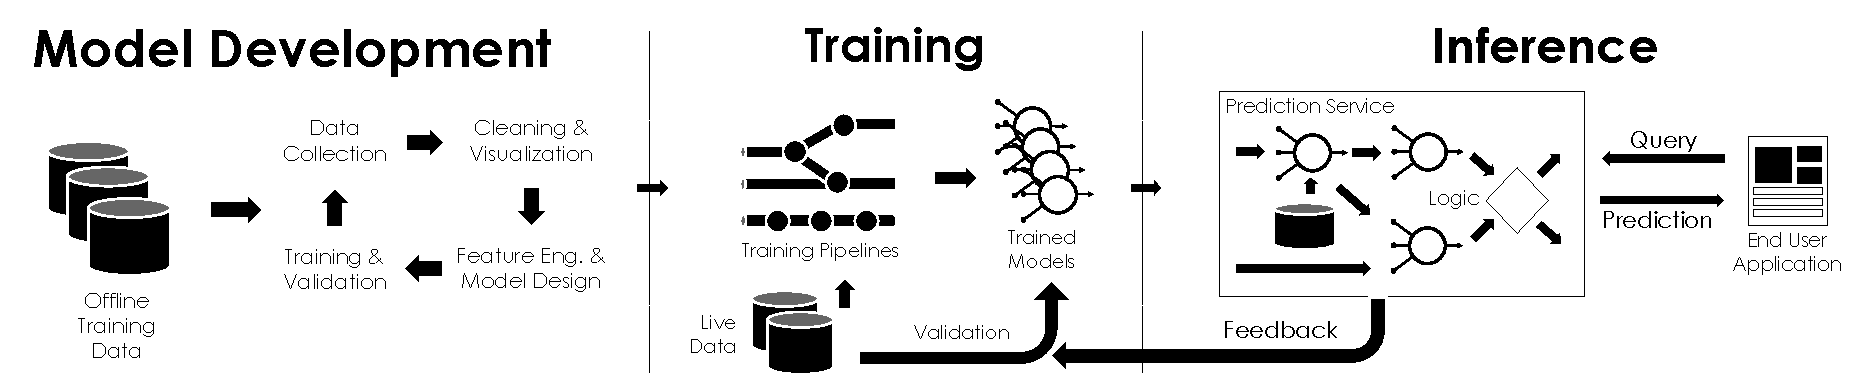
\includegraphics[width=\textwidth]{letters/pipeline.pdf}
\caption{\small \textbf{Machine Learning Life-cycle.} A simplified depiction of the key stages of a machine learning application.}
\label{fig:mllc}
\end{figure}


The machine learning life-cycle (Fig.~\ref{fig:mllc}) spans not only the model development, but also production training and inference.
Each stage demands different skills (e.g., neural network design, data management, and cluster management) and imposes different requirements on the underlying systems.
Yet there is an overwhelming need for unifying design principles and technologies to address pervasive problems including: feature management, data provenance, pipeline reproducibility, low-latency serving, and prediction monitoring just to name a few.


There has been substantial recent progress in systems to aid in managing the machine learning life-cycle.  
Large industrial projects like 
FB Learner Flow 
% \href{https://code.fb.com/core-data/introducing-fblearner-flow-facebook-s-ai-backbone/}{FB Learner Flow}
from Facebook, 
Michelangelo 
% \href{https://eng.uber.com/michelangelo/}{Michelangelo} 
from Uber, and 
TFX 
% \href{https://www.tensorflow.org/tfx/}{TFX} 
from Google have received a considerable of recent attention.  
In this issue we have solicited publications from several more recent industrial and academic projects.

The first paper, by a team at Amazon Research, provides an overview of several real-world use cases and then outlines the key conceptual, data management, and engineering challenges faced in production machine learning systems.
Rather than advocating a single system, this work describes some design principles that can inform potential solutions.


The second and third papers explores the challenges of model management and provenance across the machine learning life-cycle.
They motivate the need for systems to track models and their meta-data to improve reproducibility, collaboration, and governance. 
% expands upon the machine learning life-cycle 
% to include: data preparation, feature engineering, model training, deployment, and maintenance
% and explores the challenges of model 
The second paper introduces, ModelDB, an open-source system for model management and describe some of the functionality and design decisions. 
The third paper describes a related system, ProvDB, that uses a graph data model to capture and query fine-grained versioned lineage of data, scripts, and artifacts throughout the data analysis process.


The fourth paper, by a team at Databricks Inc., describes, MLFlow, a new open-source system to address the challenges of experimentation, reproducibility, and deployment. 
This work leverages containerization to capture the model development environment and a simple tracking API to enable experiment tracking.
The extensible model containerization enables model developers to more easily collaborate around modeling environments and then deploy model containers.


The last paper, by a team at Microsoft, focuses on inference and explores the challenges and opportunities of serving white-box prediction pipelines.  
In contrast to the containerization of pipelines in MLFlow, the Microsoft team leverage knowledge about the internal of the prediction pipeline to more efficient serve predictions. 



\end{document}



%\end{news}


%\end{newssection}

%\begin{newssection}{TCDE Election}

% there will be other letters- and a blank page will appear in your document
% but the special issue part will be fine

%\begin{news}{Letter from the Editor-in-Chief}
%{David Lomet}{Microsoft Corporation}
%\documentclass[11pt]{article} 

\usepackage{deauthor,times,graphicx}
%\usepackage{url}
\usepackage{hyperref}

\begin{document}

\subsection*{ICDE 2018}

Repeating my comment from the last issue-

The IEEE International Conference on Data Engineering will be held in April 14-19, 2018 in Paris, France.  This is the flagship conference of the Computer Society's Technical Committee on Data Engineering.  It is a great conference, at a great location.  What could possibly be better than April in Paris at ICDE!  I am attending and hope to see you there.

\subsection*{About the Bulletin}

This March current issue marks the end of editorial tenure for the Bulletin's current set of editors.  So it is once again time for me to pat myself on the back.  This current set, Tim Kraska, Tova Milo, and Haixun Wang, continue my outstanding success (he says modestly) in finding and choosing great editors.  All three have done truly fine jobs at producing issues that bring to our readers surveys of the latest work in very current areas. The success of the Bulletin depends on great issue editors.  I want to thank Tim, Tova, and Haixun for being exactly that with the fine jobs that they have done.  There was unexpected ``scrambling" over the past two years, so I want to thank them also for their flexibility in coping with this.  


\subsection*{The Current Issue}

Don't you get tired of someone shouting ``FAKE NEWS!".  Or perhaps even worse, being exposed to fake news before it has been labeled as such?  Our political conversations seem increasingly to include many variations of ``fake news" and discussions about which news is fake.  ``Sad." So where am I going with this?

The database world has been working on a key aspect of this problem for many years.  The technical area is called ``data provenance".  And it addresses the problem of where information comes from and how it impacts the subsequent processing of data and the reported results.  The June, 2010 issue was the last one on provenance.  And seven years is a long time in an active technical area, especially an area as important as this.

The current issue is focused on the applications of provenance.  Without delving into the current political scene, a reader will clearly see how extensively provenance management can be used.  As we gain more insight into its application scenarios, we also gain more insight into how to manage provenance.  This symbiotic relationship is driving the field forward.   Tova Milo, our Bulletin editor for the issue, has done an excellent job in bringing the issue together, making it a great place to learn about and track progress in the field.  The result is an issue well worth reading.



\end{document}



%\end{news}
%
%\newpage
%
%% your introductory letter goes here
%
%\begin{news}{Letter from the Special Issue Editor}
%{Joseph E. Gonzalez}{University of California at Berkeley\\ Berkeley, CA}
%\documentclass[11pt]{article} 

\usepackage{deauthor,times,graphicx}
%\usepackage{url}
\usepackage{hyperref}



\begin{document}

Machine learning is rapidly maturing into an engineering discipline at the center of a growing range of applications.
This widespread adoption of machine learning techniques poses a new set challenges around the management of the data, code, models, and their relationship throughout the machine learning life-cycle.
In this issue of the Data Engineering Bulletin we have solicited work from both academic and industrial leaders in the data engineering community that are exploring how data engineering techniques can be used to address the challenges of the machine learning life-cycle.




\begin{figure}[h]
\centering
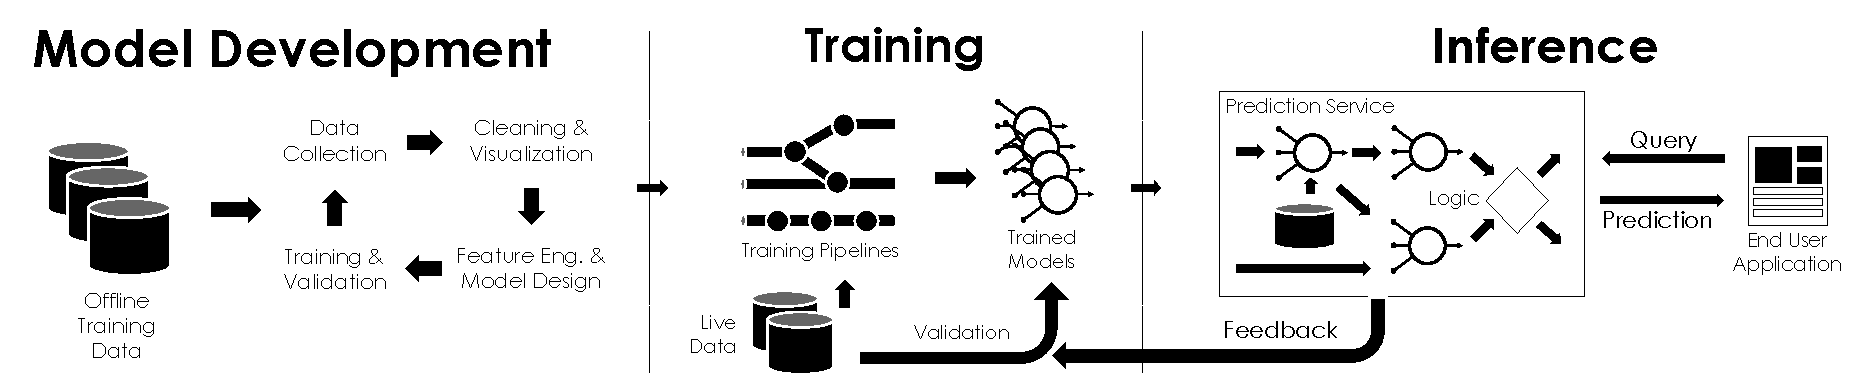
\includegraphics[width=\textwidth]{letters/pipeline.pdf}
\caption{\small \textbf{Machine Learning Life-cycle.} A simplified depiction of the key stages of a machine learning application.}
\label{fig:mllc}
\end{figure}


The machine learning life-cycle (Fig.~\ref{fig:mllc}) spans not only the model development, but also production training and inference.
Each stage demands different skills (e.g., neural network design, data management, and cluster management) and imposes different requirements on the underlying systems.
Yet there is an overwhelming need for unifying design principles and technologies to address pervasive problems including: feature management, data provenance, pipeline reproducibility, low-latency serving, and prediction monitoring just to name a few.


There has been substantial recent progress in systems to aid in managing the machine learning life-cycle.  
Large industrial projects like 
FB Learner Flow 
% \href{https://code.fb.com/core-data/introducing-fblearner-flow-facebook-s-ai-backbone/}{FB Learner Flow}
from Facebook, 
Michelangelo 
% \href{https://eng.uber.com/michelangelo/}{Michelangelo} 
from Uber, and 
TFX 
% \href{https://www.tensorflow.org/tfx/}{TFX} 
from Google have received a considerable of recent attention.  
In this issue we have solicited publications from several more recent industrial and academic projects.

The first paper, by a team at Amazon Research, provides an overview of several real-world use cases and then outlines the key conceptual, data management, and engineering challenges faced in production machine learning systems.
Rather than advocating a single system, this work describes some design principles that can inform potential solutions.


The second and third papers explores the challenges of model management and provenance across the machine learning life-cycle.
They motivate the need for systems to track models and their meta-data to improve reproducibility, collaboration, and governance. 
% expands upon the machine learning life-cycle 
% to include: data preparation, feature engineering, model training, deployment, and maintenance
% and explores the challenges of model 
The second paper introduces, ModelDB, an open-source system for model management and describe some of the functionality and design decisions. 
The third paper describes a related system, ProvDB, that uses a graph data model to capture and query fine-grained versioned lineage of data, scripts, and artifacts throughout the data analysis process.


The fourth paper, by a team at Databricks Inc., describes, MLFlow, a new open-source system to address the challenges of experimentation, reproducibility, and deployment. 
This work leverages containerization to capture the model development environment and a simple tracking API to enable experiment tracking.
The extensible model containerization enables model developers to more easily collaborate around modeling environments and then deploy model containers.


The last paper, by a team at Microsoft, focuses on inference and explores the challenges and opportunities of serving white-box prediction pipelines.  
In contrast to the containerization of pipelines in MLFlow, the Microsoft team leverage knowledge about the internal of the prediction pipeline to more efficient serve predictions. 



\end{document}



%\end{news}

%\end{newssection}



\begin{callsection}
%  This section will be empty for your version
%
%  Calls for papers section.  Use the callsection environment.
%  Each call for papers is contained in an call environment, where the single 
%  required options to \begin{call} is the name of the conference.
%
\begin{call}{ICDE 2019 Conference}
\centerline{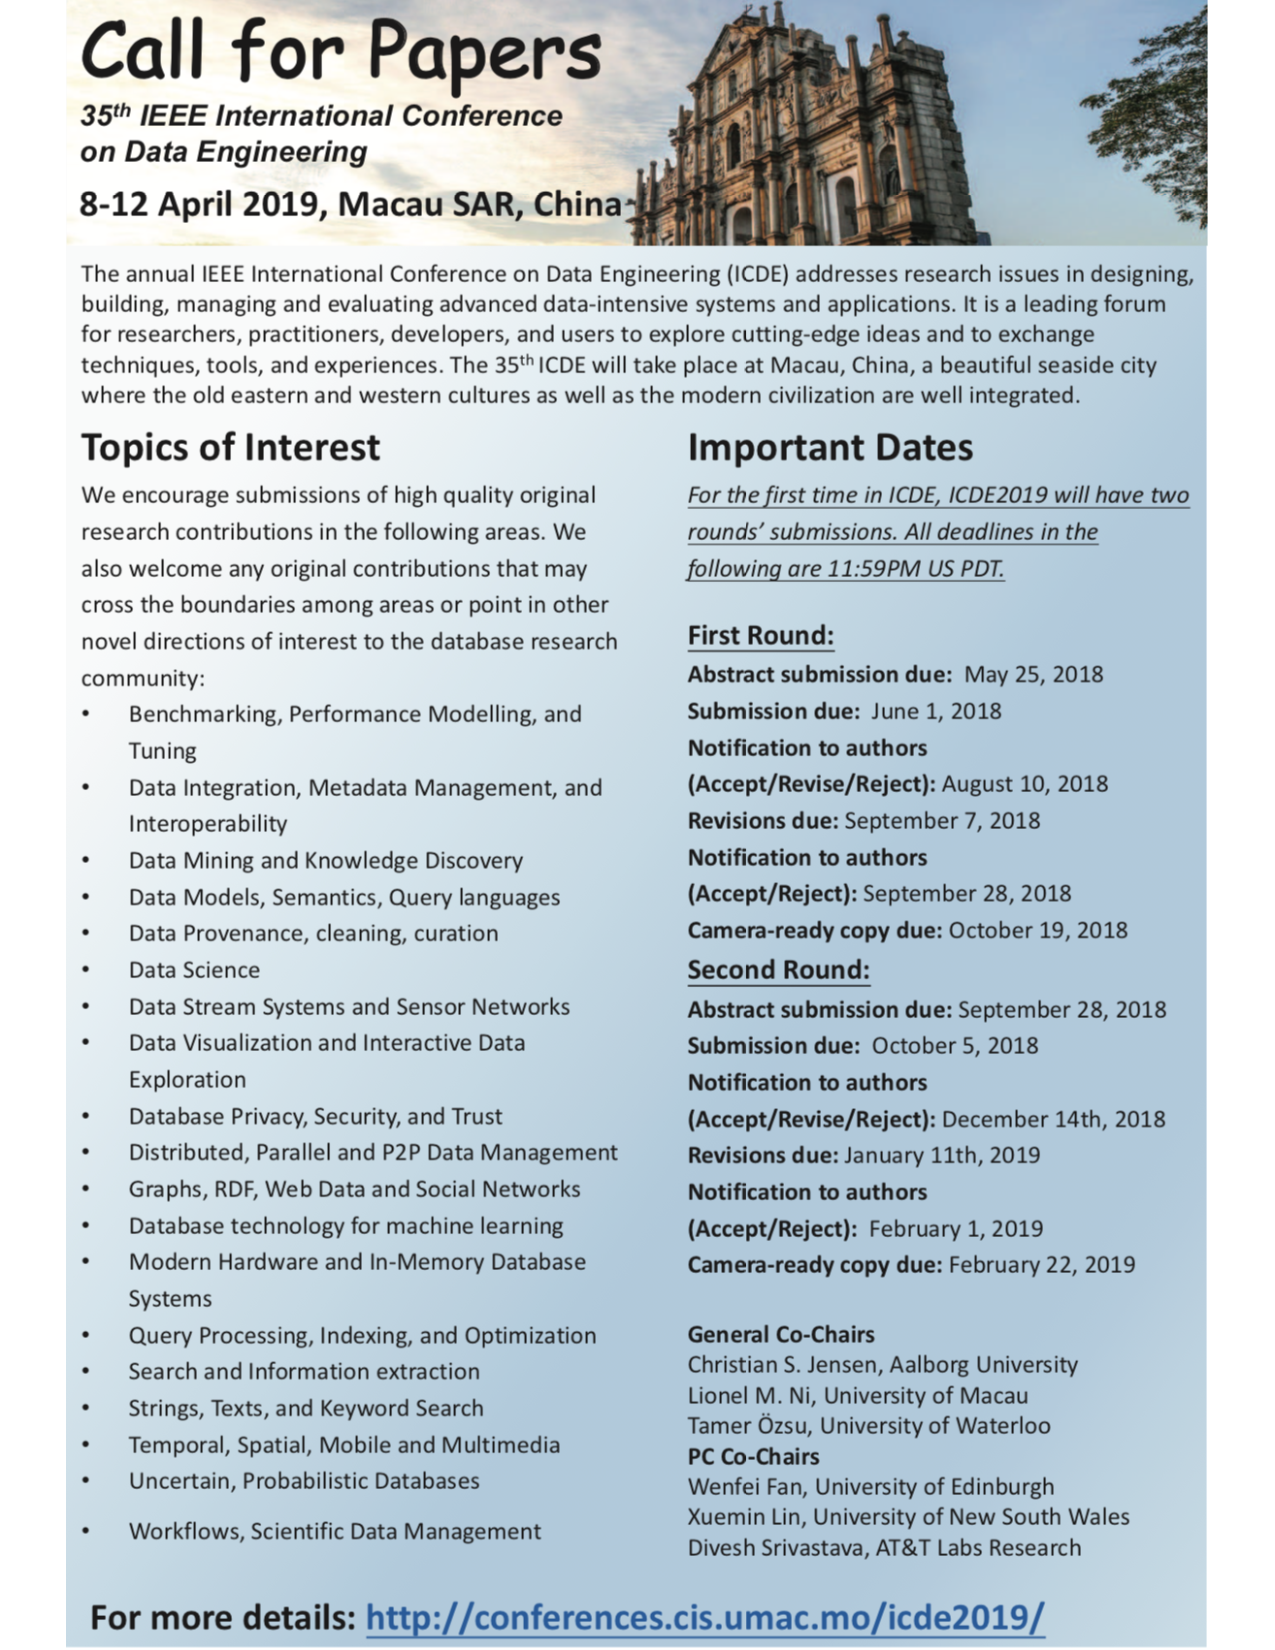
\includegraphics[width=\textwidth, bb= 0 0 610 790] {calls/icde19.pdf}} 
%\centerline{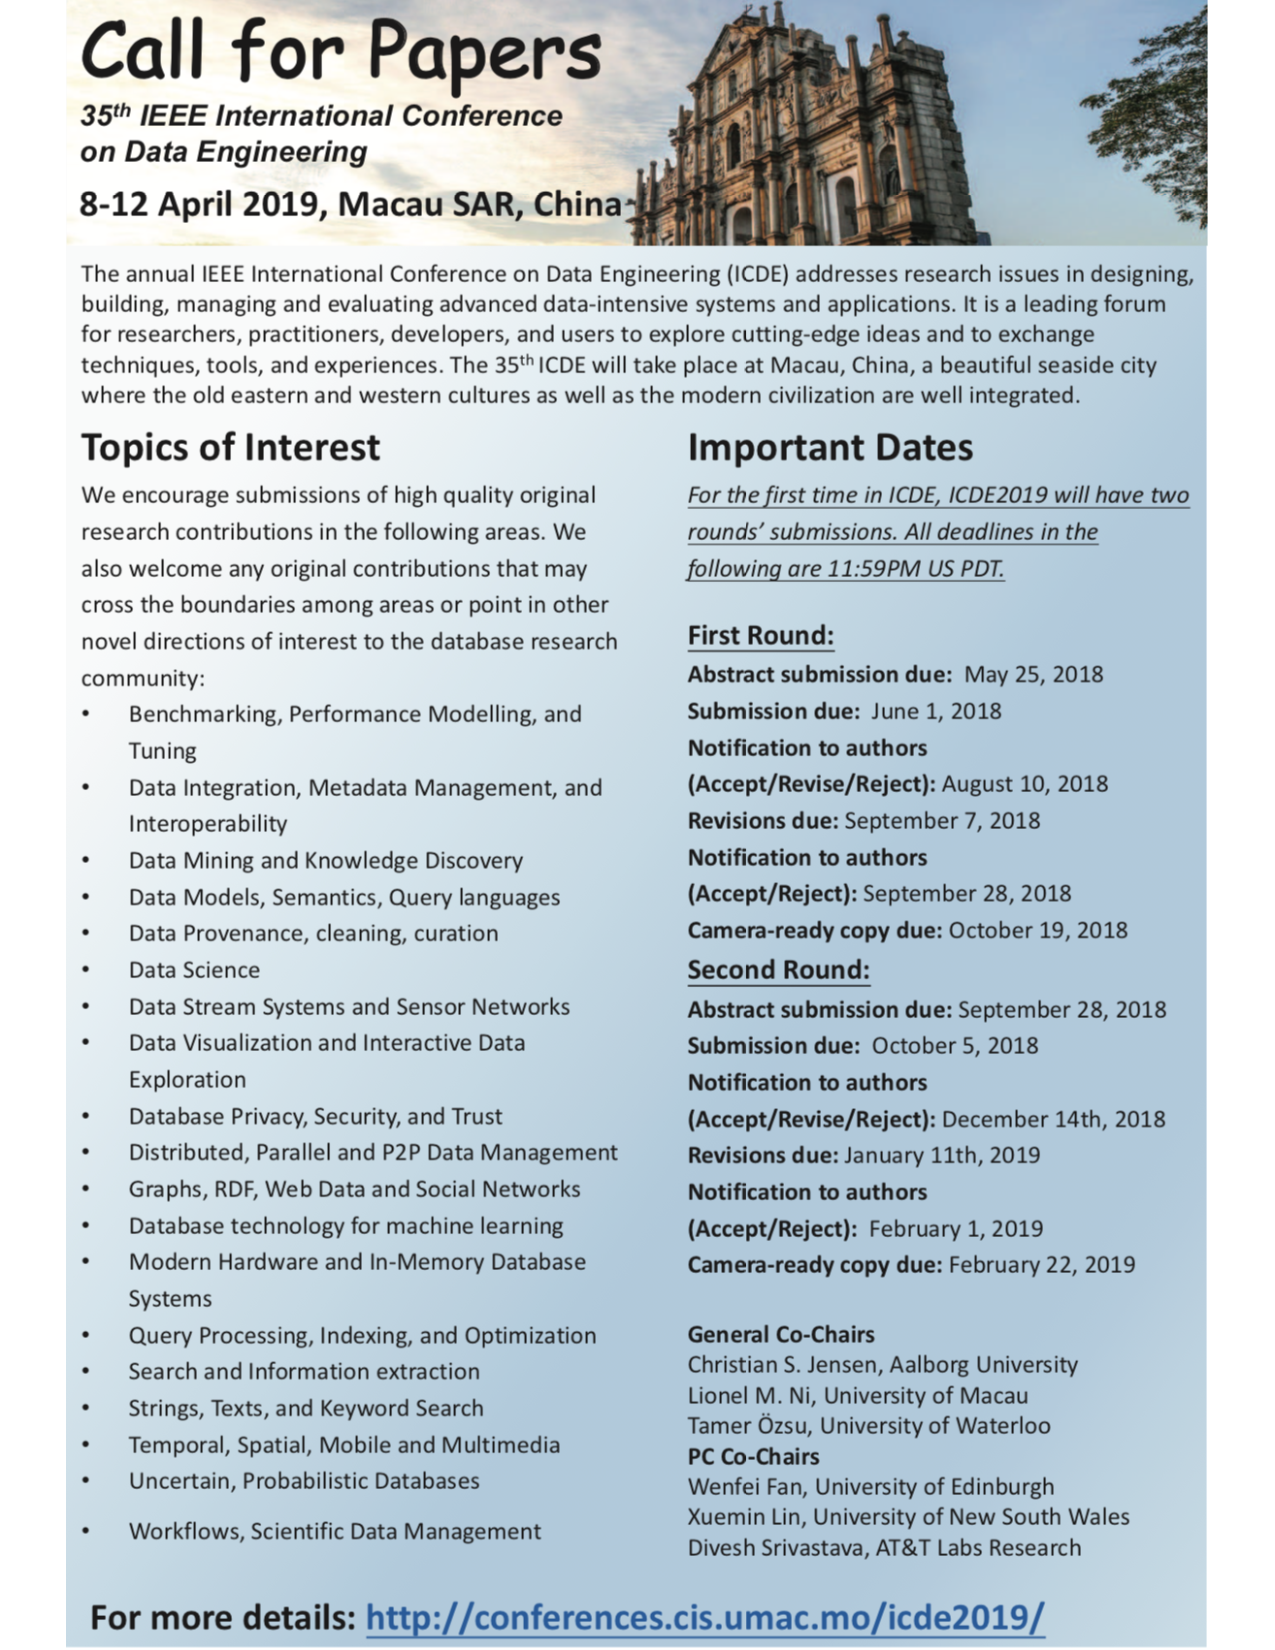
\includegraphics[width=\textwidth, bb= 0 0 590 760] {calls/icde19.pdf}}
\end{call}
\begin{call}{TCDE Membership Form}
%\centerline{\includegraphics[width=\textwidth, bb= 0 0 610 790]
\centerline{
\includegraphics[width=\textwidth, bb= 0 0 590 760] {calls/tcde.pdf}}
\end{call}
\end{callsection}

\end{bulletin}
\end{document}
